\documentclass[a4paper,11pt,twoside]{report}
\title{Intermediate Language for JavaScript Final Report}




%%%%%%%%%%%%%%%%%%%%%%%%%%%%%%%%%%%%%%%%%%%%%%%%%%%%%%%%%%%%%%%%%%%%%%%%%%%%%

% Definitions for the title page
% Edit these to provide the correct information
% e.g. \newcommand{\reportauthor}{Timothy Kimber}

\newcommand{\reporttitle}{Intermediate Language for JavaScript}
\newcommand{\reportauthor}{Aubrianna Zhu}
\newcommand{\supervisor}{Philippa Gardner}
\newcommand{\degreetype}{Computing Science}

%%%%%%%%%%%%%%%%%%%%%%%%%%%%%%%%%%%%%%%%%%%%%%%%%%%%%%%%%%%%%%%%%%%%%%%%%%%%%

% load some definitions and default packages
%%%%%%%%%%%%%%%%%%%%%%%%%%%%%%%%%%%%%%%%%
% University Assignment Title Page 
% LaTeX Template
% Version 1.0 (27/12/12)
%
% This template has been downloaded from:
% http://www.LaTeXTemplates.com
%
% Original author:
% WikiBooks (http://en.wikibooks.org/wiki/LaTeX/Title_Creation)
%
% License:
% CC BY-NC-SA 3.0 (http://creativecommons.org/licenses/by-nc-sa/3.0/)
% 
%
%%%%%%%%%%%%%%%%%%%%%%%%%%%%%%%%%%%%%%%%%
%----------------------------------------------------------------------------------------
%	PACKAGES AND OTHER DOCUMENT CONFIGURATIONS
%----------------------------------------------------------------------------------------
%\usepackage[a4paper,hmargin=2.8cm,vmargin=2.0cm,includeheadfoot]{geometry}
\usepackage[left=2.5cm,right=2cm,top=2cm,bottom=2cm,includeheadfoot]{geometry}
\usepackage{textpos}
\usepackage{natbib} % for bibliography
\usepackage{tabularx,longtable,multirow,subfigure,caption}%hangcaption
\usepackage{fncylab} %formatting of labels
\usepackage{fancyhdr} % page layout
\usepackage{url} % URLs
\usepackage[english]{babel}
\usepackage{amsmath}
\usepackage{amssymb}
\usepackage{graphicx}
\usepackage{mathpartir}
\usepackage{listings}
\usepackage{dsfont}
\usepackage{epstopdf} % automatically replace .eps with .pdf in graphics
\usepackage{backref} % needed for citations
\usepackage{array}
\usepackage{latexsym}
\usepackage{changepage}
\usepackage{algorithm}
\usepackage{algorithmic}
\usepackage{multicol}
\usepackage{smartdiagram}
\usepackage[pdftex,pagebackref,hypertexnames=false,colorlinks]{hyperref} % provide links in pdf

\addtolength{\skip\footins}{11pt}

\newcommand{\myor}{\hspace{3pt}|\hspace{3pt}}

\lstdefinestyle{mystyle}{
    basicstyle=\footnotesize,
    breakatwhitespace=false,         
    breaklines=true,                 
    captionpos=b,                    
    keepspaces=true,                 
    numbers=left,                    
    numbersep=5pt,                  
    showspaces=false,                
    showstringspaces=false,
    showtabs=false,                  
    tabsize=2
}
 
\lstset{style=mystyle}

\hypersetup{pdftitle={},
  pdfsubject={}, 
  pdfauthor={},
  pdfkeywords={}, 
  pdfstartview=FitH,
  pdfpagemode={UseOutlines},% None, FullScreen, UseOutlines
  bookmarksnumbered=true, bookmarksopen=true, colorlinks,
    citecolor=black,%
    filecolor=black,%
    linkcolor=black,%
    urlcolor=black}

\usepackage[all]{hypcap}


%\usepackage{color}
%\usepackage[tight,ugly]{units}
%\usepackage{float}
%\usepackage{tcolorbox}
%\usepackage[colorinlistoftodos]{todonotes}
% \usepackage{ntheorem}
% \theoremstyle{break}
% \newtheorem{lemma}{Lemma}
% \newtheorem{theorem}{Theorem}
% \newtheorem{remark}{Remark}
% \newtheorem{definition}{Definition}
% \newtheorem{proof}{Proof}


%%% Default fonts
\renewcommand*{\rmdefault}{bch}
\renewcommand*{\ttdefault}{cmtt}



%%% Default settings (page layout)
%\setlength{\parindent}{0em}  % indentation of paragraph

\setlength{\headheight}{14.5pt}
\pagestyle{fancy}
\renewcommand{\chaptermark}[1]{\markboth{\chaptername\ \thechapter.\ #1}{}} 

\fancyfoot[ER,OL]{\sffamily\textbf{\thepage}}%Page no. in the left on odd pages and on right on even pages
\fancyfoot[OC,EC]{\sffamily }
\renewcommand{\headrulewidth}{0.1pt}
\renewcommand{\footrulewidth}{0.1pt}
\captionsetup{margin=10pt,font=small,labelfont=bf}


%--- chapter heading

\def\@makechapterhead#1{%
  \vspace*{10\p@}%
  {\parindent \z@ \raggedright \sffamily
    \interlinepenalty\@M
    \Huge\bfseries \thechapter \space\space #1\par\nobreak
    \vskip 30\p@
  }}

%---chapter heading for \chapter*  
\def\@makeschapterhead#1{%
  \vspace*{10\p@}%
  {\parindent \z@ \raggedright
    \sffamily
    \interlinepenalty\@M
    \Huge \bfseries  #1\par\nobreak
    \vskip 30\p@
  }}

\allowdisplaybreaks

% load some macros
% Here, you can define your own macros. Some examples are given below.

\newcommand{\R}[0]{\mathds{R}} % real numbers
\newcommand{\Z}[0]{\mathds{Z}} % integers
\newcommand{\N}[0]{\mathds{N}} % natural numbers
\newcommand{\C}[0]{\mathds{C}} % complex numbers
\renewcommand{\vec}[1]{{\boldsymbol{{#1}}}} % vector
\newcommand{\mat}[1]{{\boldsymbol{{#1}}}} % matrix


\date{\today}

% Comments
\newif\ifComments
\Commentstrue

% Aubrianna
\newcommand{\az}[1]{%
\ifComments
\begin{center}
\fbox{%
\begin{minipage}{3in} \color{red}
{\bf AZ:} {\rm #1}
\end{minipage}
}
\end{center}
\fi
}

% Petar
\newcommand{\pmax}[1]{%
\ifComments
\begin{center}
\fbox{%
\begin{minipage}{3in} \color{blue}
{\bf PM:} {\rm #1}
\end{minipage}
}
\end{center}
\fi
}

\definecolor{ltblue}{rgb}{0,0.4,0.4}
\definecolor{dkblue}{rgb}{0,0.2,0.7}
\definecolor{dkgreen}{rgb}{0,0.4,0}
\definecolor{dkviolet}{rgb}{0.3,0,0.5}
\definecolor{dkred}{rgb}{0.6,0,0}
\definecolor{talkred}{rgb}{0.69,.20,0.22}
\definecolor{talkblue}{rgb}{0.04,0.40,0.80}
\definecolor{talkgreen}{rgb}{0.34,.81,0.10}
\definecolor{oldtalkblue}{rgb}{0.22,.20,0.69}
\definecolor{greenish}{rgb}{.0,.65,.0}

%JavaScript - pretty
\definecolor{SkyBlue}{rgb}{0.20,0.39,0.64}
\definecolor{Plum}{rgb}{0.46,0.31,0.48}
\definecolor{Chocolate}{rgb}{0.75,0.49,0.07}
\definecolor{Aluminium5}{rgb}{0.33,0.34,0.32}
\definecolor{DarkGreen}{rgb}{0.2,0.5,0.2}

\lstdefinelanguage{JavaScript}{
  morekeywords=[1]{typeof, new, true, false, catch,
    function, return, null, catch, switch, var,
    if, in, while, do, else, case, break, continue},
  morekeywords=[2]{class, export, boolean, throw, implements, import, this},
  numbers=left,
  numbersep=4pt,
  numberstyle=\tiny\color{dkblue},
  columns=fullflexible,
  sensitive=false,
  comment=[l]{//},
  captionpos=b,   
  morecomment=[s]{/*}{*/},
  morestring=[b]',
  morestring=[b]",
  basicstyle=\scriptsize\texttt,
  identifierstyle=\ttfamily\color{Aluminium5},
  keywordstyle=[1]\ttfamily\color{Plum},
  keywordstyle=[2]\ttfamily\color{SkyBlue},
  stringstyle=\ttfamily\color{DarkGreen},
  commentstyle=\ttfamily
}[keywords,comments,strings]

\lstnewenvironment{lstjs}{\lstset{language=JavaScript,basicstyle=\fontsize{8}{8}\ttfamily,escapeinside={~}{~}}}{}
\def\jsinline{\lstinline[language=JavaScript, basicstyle=\small]}%\end{lstlisting}

\lstdefinelanguage{JSIL}{
  morekeywords=[1]{proc, ret, err, with, goto, {l-nth}},
  numbers=left,
  numbersep=4pt,
  numberstyle=\tiny\color{dkblue},
  columns=fullflexible,
  sensitive=false,
  comment=[l]{//},
  captionpos=b,   
  morecomment=[s]{/*}{*/},
  morestring=[b]',
  morestring=[b]",
  basicstyle=\scriptsize\texttt,
  identifierstyle=\ttfamily\color{Aluminium5},
  keywordstyle=[1]\ttfamily\color{Plum},
  keywordstyle=[2]\ttfamily\color{SkyBlue},
  stringstyle=\ttfamily\color{DarkGreen},
  commentstyle=\ttfamily
}[keywords,comments,strings]

\lstnewenvironment{lstjsil}{\lstset{language=JSIL,basicstyle=\fontsize{8}{8}\ttfamily,escapeinside={~}{~}}}{}
\def\jsilinline{\lstinline[language=JSIL, basicstyle=\small]}%\end{lstlisting}

\tikzset{
  box/.style = {rectangle, draw=black,align=center,font=\scriptsize},
  sbox/.style = {rectangle,draw=black,align=center,font=\scriptsize,text width=2.3cm},
  p/.style = {-latex},
  dp/.style = {latex-latex},
  sz/.style n args={2}{minimum width=#2, minimum height=#1},
  m/.style = {midway,inner sep=0pt,fill=white},
  ll/.style = {font=\scriptsize,anchor=south west}
}

\begin{document}

% load title page
% Last modification: 2015-08-17 (Marc Deisenroth)
\begin{titlepage}

\newcommand{\HRule}{\rule{\linewidth}{0.5mm}} % Defines a new command for the horizontal lines, change thickness here


%----------------------------------------------------------------------------------------
%	LOGO SECTION
%----------------------------------------------------------------------------------------


\includegraphics[width = 4cm]{imperial.pdf}\\[0.5cm] 

\center % Center remainder of the page

%----------------------------------------------------------------------------------------
%	HEADING SECTIONS
%----------------------------------------------------------------------------------------

\textsc{\Large Imperial College London}\\[0.5cm] 
\textsc{\large Department of Computing}\\[0.5cm] 

%----------------------------------------------------------------------------------------
%	TITLE SECTION
%----------------------------------------------------------------------------------------

\HRule \\[0.4cm]
{ \huge \bfseries \reporttitle}\\ % Title of your document
\HRule \\[1.5cm]
 
%----------------------------------------------------------------------------------------
%	AUTHOR SECTION
%----------------------------------------------------------------------------------------

\begin{minipage}{0.4\textwidth}
\begin{flushleft} \large
\emph{Author:}\\
\reportauthor
\end{flushleft}
\end{minipage}
~
\begin{minipage}{0.4\textwidth}
\begin{flushright} \large
\emph{Supervisor:} \\
\supervisor % Supervisor's Name
\end{flushright}
\end{minipage}\\[4cm]


%----------------------------------------------------------------------------------------
%	FOOTER & DATE SECTION
%----------------------------------------------------------------------------------------
\vfill % Fill the rest of the page with whitespace

\includegraphics[width=6cm]{imperial2.pdf}
\vspace{0.5cm}

Submitted in partial fulfillment of the requirements for the MSc degree in
\degreetype~of Imperial College London\\[0.5cm]

\makeatletter
\@date 
\makeatother


\end{titlepage}


% page numbering etc.
\pagenumbering{roman}
\clearpage{\pagestyle{empty}\cleardoublepage}
\setcounter{page}{1}
\pagestyle{fancy}

%%%%%%%%%%%%%%%%%%%%%%%%%%%%%%%%%%%%
\begin{abstract}
JavaScript plays an increasingly important role in programming on the web, and a reliable JavaScript verification tool that could help programmers write correct and secure code remains much to be desired. As JavaScript is a dynamic object-oriented language, analysis of the behavior of JavaScript programs poses great difficulty, and is more easily accomplished using simpler intermediate languages that replicate the actions performed in JavaScript. JSIL, an intermediate language for JavaScript, has been developed for exactly this purpose.

This project extends the implementation of JSIL to include various built-in methods in the Object, Array, and String libraries, as well as the arguments object construct. The language in the 5\textsuperscript{th} edition of the JavaScript specification has been faithfully followed during JSIL implementation to ensure its correctness. When the specification is vague and up to interpretation, operational semantics is utilized to ensure clarity of method actions. All JSIL code written is concurrently tested first using manually constructed unit tests, then using an automatic testing framework, which lends itself to manual analysis. The testing framework pulls test cases from the official ECMAScript test suite, and all methods implemented have passed all the tests within the scope of this project.
\end{abstract}

\cleardoublepage
%%%%%%%%%%%%%%%%%%%%%%%%%%%%%%%%%%%%
\section*{Acknowledgments}
I sincerely thank my supervisor, Professor Philippa Gardner, for her guidance and encouragement throughout my entire project. Her insights were invaluable, and this project could not have taken a better direction.

I would also like to thank Jos\'e Fragoso Santos for setting up my programming environment and explaining logical concepts. I would like to thank Thomas Wood for creating and maintaining the testing framework. And I would like to thank Iv\'an Matellanes for some quick bug-fixing.

Lastly, my most heartfelt thanks goes to Petar Maksimovi\'c, who supervised my learning of JSIL and spent countless hours troubleshooting and reviewing my work. 

\clearpage{\pagestyle{empty}\cleardoublepage}

%%%%%%%%%%%%%%%%%%%%%%%%%%%%%%%%%%%%
%--- table of contents
\fancyhead[RE,LO]{\sffamily {Table of Contents}}
\tableofcontents 


\clearpage{\pagestyle{empty}\cleardoublepage}
\pagenumbering{arabic}
\setcounter{page}{1}
\fancyhead[LE,RO]{\slshape \rightmark}
\fancyhead[LO,RE]{\slshape \leftmark}

%%%%%%%%%%%%%%%%%%%%%%%%%%%%%%%%%%%%
\chapter{Introduction}
\label{cha:intro}

\section{Thesis Project}
To determine whether or not a computer program is behaving correctly, simply eyeballing it is no longer enough and stronger guarantees are required. There is a need for verification tools that analyse and prove the correctness of computer programs. This thesis contributes towards the end goal of creating a verification tool for the JavaScript programming language. This is accomplished by building on previous work on the JSIL intermediate language and the JS-2-JSIL compiler from JavaScript to JSIL, which was done in the Program Specification and Verification Group at Imperial College London. We substantially extend the coverage of the JS-2-JSIL compiler and evaluate this extension by systematically testing against the ECMAScript Test262 test suite to prove the correctness of our implementation.

In order to achieve the goals of this project, significant preparations were undertaken. The first hurdle was operational semantics, which involved self-studying the first four lectures of the second-year Models of Computation course and the ECMAScript operational semantics written for the internal functions of JavaScript. Learning the language of symbolic representations was difficult without a strong foundation in logic. The second challenge was understanding a programming language specification, namely the ECMAScript 5 standard for JavaScript, and understanding in detail the complexity of JavaScript at a low level. Lastly, extensive practice coding in JSIL, a goto-style intermediate language, was necessary for implementing all of the extensions.

As part of this project, we have implemented in JSIL the Object.prototype and the Array libraries in full, as well a subset of the String library. The Object.prototype library encompasses seven built-in methods for two pages in the ECMAScript standard; the Array library includes twenty-eight built-in methods for a total of twenty pages; and the subset of String library includes six built-in methods for four pages. The \jsinline|arguments| object, a core JavaScript construct encompassing three pages of the standard, has been implemented as well. The implementation of all of these libraries and constructs amounts to more than two thousand lines of JSIL code, and was systematically tested both against manually written unit tests, as well as the standard ECMAScript Test262 test suite.

The current testing framework includes the entire ECMAScript 6 test suite (ES6 Test262) which consists of 21301 test cases, but essentially targets the 11037 tests suitable for ES5 Strict, which is the mode of JavaScript targeted by the JS-2-JSIL compiler. The remaining ones, such as those aimed at ES6-only and non-strict features are filtered out. At the starting point of this project, there were 5574 relevant tests passing. After the completion of this project, there were 2263 additional tests passes, yielding a total of 7837 total tests passes, which constitutes a 40\% increase.

%The interactive testing framework is available online from a publicly accessible web address and is continuously integrated into the JSIL project. Each JSIL commit can be viewed from the testing portal, and the results can be compared with previous commits to determine whether the commit improved or worsened test coverage. JSIL development and testing will be done concurrently, and mistakes will be spotted and addressed as soon as they appear.

\section{What is JavaScript?}
JavaScript is the unofficial language of the Web---it is implemented in all major browsers, and its main purpose is to add interactivity to web pages by giving the programmer control over the browser's Document Object Model,~i.e.~both the pages' style and their content. In addition, JavaScript is increasingly used on the server side as well, primarily as a means of interacting with databases. It is a high-level, dynamic, untyped language, based on extensible objects and exhibiting a number of intricate, complex, and often unpredictable features. 

For example, JavaScript supports prototypical inheritance rather than class inheritance, which is favoured by many object-oriented programming languages, such as Java and C++. It allows for first-class functions, i.e.~functions that can be passed as parameters to other functions, and also for partial function application. It features implicit, silent coercions between numbers, strings, booleans, and objects, which are the source of numerous programming errors that can at times be exceptionally difficult to debug.
Also, JavaScript does not have static typing or require type declarations~\cite{EcmaScript}. As an illustration of the complexity of JavaScript, the following is a seemingly strange, but valid, JavaScript expression:

$$\jsinline|(![]+[])[+!+[]]|$$

\noindent which, remarkably, evaluates to the string \jsinline|"a"|; discussion of how this particular evaluation is performed, as well as the above-mentioned intricacies of JavaScript will be presented in detail in Chapter~\ref{sec:javascript}.

JavaScript was developed, and is still being improved and updated, by the ECMAScript committee. The committee is in charge of publishing the ECMAScript standard, addressing the language syntax, semantics, libraries, and complementary technologies that support the language. Since its inception, six versions of the standard have been developed, with the latest one having been released in June 2015 \cite{international2015ecmascript}. This project will primarily target the 5\textsuperscript{th} edition of the ECMAScript standard, which was published in 2011, while discussing some of the differences between itself and its predecessor, ECMAScript 3, as well as its successor, ECMAScript 6.

\section{The Importance of Verification}\label{sec:jsspec}
Computer scientists have created high-level programming languages such as JavaScript with the idea of stepping away from machine code and assembly and, instead, instructing machines to perform actions in a more human-like way. Designing a programming language is a complicated endeavour, and possibilities for mistakes exist even in the earliest stages. For instance, five years after its creation, Java, a real life programming language, was shown not to comply with type safety~\cite{drossopoulou1998towards}. It is of little help for correctness that, just like natural languages, programming languages evolve and become increasingly complicated. Moreover, programming language specifications are often written in plain prose that sometimes lacks detail or is simply ambiguous, which can result in diverging interpretations by different readers. One should contrast this with the fact that program correctness plays a crucial role in life-critical or security-critical settings, such as in the aviation or banking industries.

Therefore, when a programmer writes a piece of code that is intended to perform a certain task, without proper tools they cannot be entirely sure that their program will perform the task as required without any side effects. In order to reduce the errors and inconsistencies in different implementations of the same language, a formal verification system is necessary so that one could prove that programming languages and programs written in those languages are indeed performing correctly, as expected, with no ambiguities.

\subsection{JavaScript Verification}
Because of the dynamic nature of JavaScript, it is often difficult for programmers to fully understand JavaScript code, resulting in unexpected outcomes during program execution. A lack of adequate static analysis tools further exacerbates this situation, and this project aims to contribute to resolving the urgent need for a JavaScript verification tool. 

Indeed, a current example of web security issues related to JavaScript include cross-site scripting (XSS), that allows a hacker to inject malicious JavaScript code into a harmless web page. The malicious code is executed on the page, and it can potentially steal sensitive user information or spread viruses and malware \cite{security}. By using a verification tool, JavaScript programmers can discover security vulnerabilities, and fix them before releasing their web page to the public.

Previous work on JavaScript verification that makes this project possible includes formal reasoning about JavaScript using program logics \cite{Gardner:2012}; JSCert and JSRef, which are a mechanized specification of the ECMAScript standard and a certified reference interpreter, both written in the Coq proof assistant \cite{Bodin:2014}; and the JSIL intermediate language, which relies on JSCert and is at the core of this project. All of these works will be discussed in more detail in sections~\ref{sec:jslogic} to~\ref{sec:jsverify}.

\subsection{JS Logic}\label{sec:jslogic}
Gardner et al. \cite{Gardner:2012} have demonstrated that a program logic based on separation logic can be used to reason about JavaScript, in particular the ECMAScript 3 standard. Their main motivation for using separation logic was that this particular kind of logic is useful when reasoning about heap-manipulating programs, which is precisely how JavaScript works, as it stores the entire program state within a heap. A concept of weak locality was employed to establish the soundness of the logic, as program commands are required to be local but JavaScript commands are not \cite{Gardner:2012}. The soundness proof was based on big step operational semantics, which was developed for most of the standard, but was simplified (e.g.~descriptors were not considered). This semantics supplements a previous effort of developing a small step operational semantics for core ECMAScript 3 functionalities by Maffeis et al. \cite{Maffeis:2008}.

\subsection{JSCert and JSRef}\label{sec:jscert}
JSCert is a mechanised specification of the ECMAScript 5 standard in the proof assistant Coq\cite{Bodin:2014}. It uses pretty-big-step semantics, covers all of the language constructs and a small part of the built-in libraries, and consists of approximately eight hundred derivation rules. These rules are of the form $t/S/C \Downarrow_s S'/o$, where $t$ is the statement being executed, $S$ is the current program state, $C$ is the current execution context, and $S'/o$ is the output, meaning that if we execute the statement $t$ starting from the state $S$ and execution context $C$, we will obtain the output $S'/o$. The output consists of the final state $S'$ and a completion triple $o$ containing the return type, the return value, and the return label \cite{Bodin:2014}. JSCert, given that it defined inductively, can be used to reason only about the scenarios where the program terminates, and not those in which it diverges. 

% number of rules

JSCert comes accompanied by JSRef, an executable reference interpreter for JavaScript, written in Coq and extracted to OCaml. JSRef contains records of functions that evaluate various parts of JavaScript source code, and recursively returns the result of program execution \cite{Bodin:2014}. JSRef is proven correct in Coq with respect to JSCert; it is also tested against the official ECMAScript Test262 test suite in order to establish the correctness of both JSRef and JSCert with respect to the  standard.

\subsection{JSVerify}\label{sec:jsverify}
For languages such as C and Java, efforts to verify program correctness have well been underway, as described in Section~\ref{sec:hist}, yielding many integrated development environments (IDEs) that perform dynamic and static analyses of code and help programmers debug their programs. Current JavaScript IDEs provide little more than simple syntax highlighting and do not adequately address program correctness. Given its highly dynamic nature, JavaScript code can often have bugs \cite{Gardner:2012} and even be vulnerable to security attacks \cite{Lee:2007}. 

The ideas presented in sections~\ref{sec:jslogic} and~\ref{sec:jscert} have led to a currently ongoing verification project called JSVerify. Its aims are to use separation logic to reason about JavaScript programs and provide proofs of their correctness. This project ties in with JSVerify in that JSVerify will actually analyse code written in the intermediate language JSIL from this project, in order to determine the correctness of the corresponding JavaScript program. This can be accomplished because there exists a proof of correctness of the translation from JavaScript to JSIL.

\section{Report Outline}
The rest of the report includes the following nine chapters.

\begin{description}
\item[Chapter 2] Gives an overview of the history behind mechanized specifications, related work, and explains operational semantics.
\item[Chapter 3] Provides detailed discussions on topics of JavaScript, including but not limited to objects, properties, and prototype inheritance.
\item[Chapter 4] Describes JSIL as an intermediate language --- its syntax and semantics.
\item[Chapter 5] Explains the JavaScript Object.prototype Library and one method in detail.
\item[Chapter 6] Provides detailed discussions on topics related to JavaScript Arrays, and explains the Array Library and two methods in detail.
\item[Chapter 7] Describes the Arguments Object in JavaScript and its JSIL implementation.
\item[Chapter 8] Explains a subset of the String Library methods.
\item[Chapter 9] Provides an explanation regarding the testing process, and provides detailed results for the JSIL implementation of the String Library methods.
\item[Chapter 10] Gives a brief conclusion of the topics studied, evaluates the project, and introduces possible future extensions.
\end{description}

%%%%%%%%%%%%%%%%%%%%%%%%%%%%%%%%%%%%
\chapter{Background} \label{cha:bckgnd}
In this chapter, we focus on the background of this thesis, including: the history and landscape of mechanised specifications for a variety of programming languages (Section \ref{sec:hist}); a detailed explanation of operational semantics, a technology for formalising the semantics of programming languages (Section \ref{sec:opsem}); a more in-depth look at the related work on JavaScript specification and verification (Section \ref{sec:jsspec}); and initial work, which predates this thesis, on translating the ECMAScript standard first into pretty-big-step operational semantics and then from this operational semantics to JSIL, an intermediate language for JavaScript verification (Section \ref{sec:opsemac}).

\section{History of Mechanised Specifications}\label{sec:hist}
There has been a long history of mechanised specification of programming languages. Initial formalisations were often simple and would not cover all of the aspects of the languages they targeted. Additionally, they tended to be non-executable and thus the appropriateness of their definitions was at times uncertain \cite{Ellison:2012}. Gradually, formalisations became increasingly mechanised, executable, and testable against standard test suites such as ECMAScript Test262 and GCC torture tests, or specific implementations such as Mozilla's JavaScript in order to ascertain actual real-life correctness of these specifications. The following subsections describe a number of mechanised specifications for various programming languages.

\subsection{ML}
\begin{description}
\item[Lee et al. 2007] This study created an internal language (IL), whose semantics is an explicitly-typed $\lambda$-calculus which follows a variation of the Harper and Stone\cite{Harper:2000} style, for standard ML \cite{Lee:2007}. This IL was able to capture all of the features in standard ML, and the proof of its type safety was successfully formalized in LF \cite{Harper:1993} and Twelf \cite{Pfenning98guide}.
\end{description}

\subsection{C}\label{sec:chist}
There have been many formal semantics written for the C programming language, ranging from those using abstract state machines \cite{Gurevich:1992} to those done in the HOL theorem proving system \cite{norrish:1998}, in addition to the two described below.
\begin{description}
\item[Leroy 2009] CompCert is a certified compiler from (almost all of) the ISO C 99 standard to PowerPC assembly code, and it was designed to address the correctness of compilers, as most formal verification is done on source code rather than on code produced by optimized compilation. It used the Coq proof assistant for formal verification, to prove that the semantics of the generated assembly code corresponds exactly to the semantics of the source code \cite{Leroy-Compcert-CACM}. This verification is accomplished using eight intermediate languages from ISO C 99 to assembly, with each transformation having a formal proof that it preserves the semantics of the previous language in the translation chain.

\item[Ellison and Rosu 2012] This work employs $\mathbb{K}$ \cite{rosu-serbanuta-2010-jlap}, a semantic framework based on rewriting-logic, and Maude \cite{Clavel:2007}, a rewriting-logic engine that enables execution and analysis of the mechanized semantics \cite{Ellison:2012}. The $\mathbb{K}$-based semantics for C is executable and was tested against the GCC torture test suite \cite{Ellison:2012}. 
\end{description}

\subsection{Java}
As for C, there exists a large body of work concerning the formalisation of Java. 
\begin{description}
\item[Drossopoulou and Eisenbach 1998] As early as 1998, a small step operational semantics has been defined for Java \cite{drossopoulou1998towards,Drossopoulou:1999} using a term rewriting system. This work has covered a substantial subset of the Java language, with a focus on proving that the type system indeed works correctly.

\item[Klein and Nipkow 2006] Another example is the work done using the Isabelle theorem prover \cite{Paulson1989}, an environment to formalise and prove the type safety for Jinja \cite{KleinN-TOPLAS}, a variation of Java. The authors utilised both small step and big step operational semantics---the two styles are used in different aspects of the proof, but they are shown to be equivalent. This work is important because it was the first holistic formal analysis of a Java-like language, its virtual machine, and its compiler \cite{KleinN-TOPLAS}.

\item[Bogdanas and Rosu 2015] The most recent work done on formalising Java follows the C example from section~\ref{sec:chist}, using $\mathbb{K}$ as the development tool for Java 1.4. In this project, all features in the Java specification were covered and tested \cite{Bogdanas:2015}, as $\mathbb{K}$ automatically provides the executable environment for the formal specification, named K-Java. 
\end{description}

\subsection{JavaScript}
This section presents four sample studies, with the first being a purely theoretical translation of the ECMAScript standard, whereas the other three also have executable portions.

\begin{description}
\item[Maffeis et al. 2008] The authors produced an extensive small step operational semantics for ECMAScript 3, encompassing about 70 pages of rules and definitions \cite{Maffeis:2008}. The main goal of this formalisation was to analyse the security properties of JavaScript programs running in web browsers, as the operational semantics allowed the authors to understand what can and cannot interact with the heap when a program is run. This operational semantics was not directly executable, but the authors designed experiments to test certain constructs on different browser implementations, and found discrepancies between Firefox, Safari, and the JavaScript standard implementation \cite{Maffeis:2008}. This work was important in inspiring other researchers to pursue operational semantics as a way to fully understand JavaScript behaviour.

\item[Politz et al. 2012] A formal semantics, S5, for the strict mode of ECMAScript 5.1 was developed following the semantics of $\lambda$\textsubscript{JS} \cite{Guha:2010}. The authors aim to cover the core semantics of JavaScript, and provide a desugaring function that compiles JavaScript code to S5. This formalisation is executable and tested for conformance with the ECMAScript test suite, Test262. S5 focuses in particular, on getters and setters, and the \texttt{eval} operator \cite{Politz:2012}.

\item[Bodin et al. 2014] In this work, the ECMAScript 5 standard was mechanised using pretty-big-step semantics (JSCert) and a reference interpreter (JSRef) was implemented using the Coq theorem prover. JSRef was proven correct with respect to JSCert, then extracted to OCaml using Coq's built-in extraction mechanism, and tested against Test262 \cite{Bodin:2014}. This correctness result ensures that both JSCert and JSRef are correct with respect to the JavaScript standard. The work done in this thesis stems from this work, and both JSCert and JSRef will be discussed in more detail in section~\ref{sec:jscert}.

\item[Park et al. 2015] Similar to the study presented in Section~\ref{sec:chist}, this formal semantics of JavaScript, called KJS, is also based on $\mathbb{K}$ \cite{k-primer-2013-v32}. KJS was tested against Test262, and its language constructs closely resemble the ECMAScript standard. In addition, it was able to discover coverage deficiencies in Test262 itself. This framework, however, does not allow reasoning on the meta-properties of JavaScript \cite{Park:2015}.
\end{description}

\subsection{Intermediate Languages for JavaScript}\label{sec:ir}
Most real-world programming languages are far too complex for any reasonable analysis, and need to be transformed to a simpler form in order for verification to take place. These simpler forms are called {\em Intermediate representations}. Historically, intermediate representations have already been used in many compilers, as a compilation step between the initial source code and the resulting assembly code \cite{Necula2002}. As the need for language verification arose, intermediate representations, in this context also called intermediate languages, found their usefulness in this field as well.

Currently, many intermediate languages exist; one of the most prominent is CIL, which targets the C programming language. Unlike C, CIL has only one looping construct, it makes the return statement explicit for all functions, and it simplifies the type system \cite{Necula2002}.

\paragraph{JavaScript Intermediate Languages}
\begin{description}
\item[JSIR] One intermediate language for JavaScript is JSIR \cite{Livshits:2016:Misc}, which aims to make different analysis tools more unified and less platform-dependent. Much of its grammar is defined, and can be found at \cite{Livshits:2016:Misc}. However, up to this point, there have been no implementations for JSIR and there is no compilation provided from any higher-level programming language to JSIR.

\item[WALA] Another interesting intermediate language, initially developed by IBM, is WALA \cite{WALA}. Unlike most other intermediate languages which are developed and used in academia, WALA is a set of full-fledged Java libraries used in production code for static and dynamic analysis of Java code. It also supports simple program analyses for JavaScript, in the form of JS-WALA \cite{WALA2}.

\item[Lambda JS / S5] $\lambda$\textsubscript{JS} \cite{Guha:2010} is a small step operational semantics that claims to capture the essential features of JavaScript (ECMAScript 3), except for the \texttt{eval} functionality. S5 extends $\lambda$\textsubscript{JS} to the ECMAScript 5 standard and focuses on JavaScript's strict mode \cite{Politz:2012}. Additional features covered by S5 include accessors and the \texttt{eval} function. JavaScript is translated to the core $\lambda$\textsubscript{JS} language via a desugaring function, and both $\lambda$\textsubscript{JS} and S5 are executable and tested against a Mozilla test suite and the Test262 suite, respectively.

\item[JSIL] is the intermediate language around which this thesis revolves. Like other intermediate languages, JSIL does not have many high-level language constructs. Instead, it is a simple $\texttt{goto}$ language with top-level procedures and labels and commands that resemble assembly code. JSIL has a memory model that is similar to that of JavaScript and this similarity helps relate JSIL programs with JavaScript programs easily.\footnote{Active work is in progress for JSIL and pending publication.} The full syntax of JSIL will be discussed in detail in Chapter~\ref{sec:jsil}.

%As seen in the heap models below, JavaScript heaps map locations, $\mathcal{L}$, and JavaScript variables, $\mathcal{X}_{JS}$, to JavaScript values, $\mathcal{V}_{JS}$, and scope chains, $\mathcal{S}ch_{JS}$, whereas JSIL heaps map locations, $\mathcal{L}$, and JavaScript variables, $\mathcal{X}_{JS}$, to JSIL values, $\mathcal{V}_{JSIL}$.

%\begin{center}
%\begin{tabular}{p{9cm}} \hline
%\textbf{JavaScript Heap Model} \\
%$\texttt{h} \in \mathcal{H}_{JS} : \mathcal{L} \times \mathcal{X}_{JS} \rightharpoonup (\mathcal{V}_{JS} \cup \mathcal{S}ch_{JS})$  \\ \hline
%\end{tabular}
%
%\begin{tabular}{p{9cm}} \hline
%\textbf{JSIL Heap Model} \\
%$\texttt{h} \in \mathcal{H}_{JSIL} : \mathcal{L} \times \mathcal{X}_{JS} \rightharpoonup \mathcal{V}_{JSIL} $  \\ \hline
%\end{tabular}
%\end{center}

\item[High-Level Languages] Lastly, there are many studies that are focusing on the high-level constructs of JavaScript rather than using intermediate representations for JavaScript verification. For example, Jensen et al. \cite{unevalizer2012} describe a way to transform JavaScript programs to eliminate the use of \texttt{eval} functions to improve static analysis of JavaScript source code. But, as these methods only verify the source programs, and not the programming language itself, they are outside the scope of this project and will not be discussed in further detail.
\end{description}

\section{Operational Semantics}\label{sec:opsem}
Similarly to natural languages, when talking about programming languages one needs to distinguish between syntax and semantics. Syntax refers to the physical structure and rules of the language, defining valid variable names and correct placement of separators; semantics refers to the meaning of the program, specifying the actions and results of program commands. In regards to verification, semantics is what makes a program correct or incorrect. There are three different categories of program semantics: denotational, axiomatic, and operational. Out of these, operational semantics is our category of choice, as it specifies meaning by giving the steps and behaviour of a program during execution \cite{PittsAM:opespe}. In general, there are two ways of representing semantics operationally: small step and big step, and we will now explain each of them in detail using the simple imperative programming language based on integer arithmetic, shown below:

$$
\arraycolsep=1.5pt
\begin{array}{rclcl}
E & \in & \mathrm{Exp} & ::= & \texttt{x} \myor \texttt{n} \myor - E \myor E + E \\
B & \in & \mathrm{Bool} & ::= & \texttt{true} \myor \texttt{false} \myor B \land B \myor \neg B \myor E = E \myor E < E \\
C & \in & \mathrm{Com} & ::= & \texttt{skip} \myor \texttt{x}:=E \myor \texttt{if B then C else C} \myor \texttt{while B do C} \myor C; C 
\end{array}
$$

\noindent where we denote variables by $\texttt{x}$ and integer literals by $\texttt{n}$. As we can see, this language has three syntactic categories: {\bfseries(1)} expressions $E$, which include variables (taking integer values), integer literals, the unary minus, and addition; {\bfseries(2)} booleans $B$, which include the standard $\mathtt{true}$ and $\mathtt{false}$ boolean literals, conjunction, negation, and the two comparison operators $=$ and $<$ on expressions; and {\bfseries(3)} commands {C}, which include the empty statement, variable assignment, the standard $\mathtt{if}$ and $\mathtt{while}$ statements, and command sequencing. We define states $s$ as mappings from variables to integers, and, finally, we define configurations as $\langle E,s \rangle$, $\langle B,s\rangle$ and $\langle C,s \rangle$, meaning expressions, booleans, and commands with respect to a given state $s$.

\subsection{Small Step Semantics}
Small step operational semantics is also called structural operational semantics, and it evaluates expressions one step at a time \cite{Lecture2}. Due to its fine granularity, small step semantics is often used to model type systems and concurrency \cite{chargueraud-13-pretty}, as well as mechanised programming language definitions. The relation between two states is represented by the $\rightarrow$ symbol, and an example of this semantics is given below. In S-LEFT, an expression is evaluated from left to right: $\mathbf{E}_1$ is evaluated before $\mathbf{E}_2$. If the left hand side is already a literal, then the expression on the right hand side, $\mathbf{E}$, will be evaluated using the S-RIGHT rule. Once all expressions have been evaluated, actual addition will occur using the S-ADD rule. Note that the underlined literals in S-ADD denote  actual natural numbers, while those that are not underlined are only symbols of our language.
\begin{mathpar}
\inferrule[S-LEFT]{\mathbf{E}_1 \rightarrow \mathbf{E}'_1}{\mathbf{E}_1 + \mathbf{E}_2 \rightarrow \mathbf{E}'_1 + \mathbf{E}_2}
\and
\inferrule[S-RIGHT] {\mathbf{E} \rightarrow \mathbf{E}'}{\text{{\texttt{n}}} + \mathbf{E} \rightarrow \text{{\texttt{n}}} + \mathbf{E}'}
\and
\inferrule[S-ADD]{\underline{\texttt{n}_1} + \underline{\texttt{n}_2} = \underline{\texttt{n}_3}}{\texttt{n}_1 + \texttt{n}_2 \rightarrow \texttt{n}_3 }
\end{mathpar}

A more concrete evaluation example, $(1 + 3) + ( 2 + 1 ) \rightarrow 4 + (2 + 1) \rightarrow 4 + 3 \rightarrow 7$, would require first the S-LEFT rule to be applied to $(1 + 3)$, then the S-ADD rule to procude 4 and give the intermediate result $4 + (2 + 1)$; next, the S-RIGHT rule needs to be applied to $(2 + 1)$ and the S-ADD rule to produce 3 to give the intermediate result $4 + 3$; finally, another application of S-ADD yields the final result, which is 7 \cite{Lecture2}.

As for the $\mathtt{while}$ command, only one rule is necessary as the semantics takes care of the recursive looping on its own. Only the initial step needs to be defined and the rule will carry on until it reaches a $\mathtt{skip}$ condition. Details for the small step evaluation rules for sequential composition and conditionals have been omitted. The following small step semantics for the $\mathtt{while}$ command is presented in the Models of Computation course at Imperial for second-year Computing students.

$$
\inferrule[SS-WHILE]{ }{\langle \texttt{while B do C, s} \rangle \rightarrow_c \langle \texttt{if B then (C; while B do C) else skip, s} \rangle}
$$

\noindent We can see that, if $B$ evaluates to $\mathtt{false}$, the loop terminates as we reach the $\mathtt{skip}$ command in the $\mathtt{else}$ branch. Otherwise, $B$ evaluates to $\mathtt{true}$ and
we {unroll} the loop once, i.e.~we execute sequentially the body $C$ of the loop (which may result in a change to the state) with the recursive call of the original $\mathtt{while}$ command. 

\subsection{Big Step Semantics}
Big step operational semantics is also called natural operation semantics, and in contrast to small step, it evaluates the entire expression in one step and returns the final result immediately \cite{Lecture2}, and the behavior of one term can be seen as the composition of the behaviors of its sub-terms \cite{chargueraud-13-pretty}. The relation between two states is commonly represented by the $\Downarrow$ symbol, and the evaluation for the addition operator is given below. In B-NUM, a number evaluates to itself. The equivalent rule does not exists in the small step semantics, because numbers are considered to be fully evaluated there. In B-ADD, $\mathbf{E}_1$ and $\mathbf{E}_2$ are evaluated separately to two numbers, $\texttt{n}_1$ and $\texttt{n}_2$, respectively, while applying actual addition in the same rule to arrive at the final answer $\texttt{n}_3$.

$$
\inferrule[B-NUM]{ }{\texttt{n} \Downarrow \texttt{n}}
\hspace*{2cm}
\inferrule[B-ADD] {\mathbf{E}_1 \Downarrow \texttt{n}_1 \\ \mathbf{E}_2 \Downarrow \texttt{n}_2 \\ \underline{\texttt{n}_1} + \underline{\texttt{n}_2} = \underline{\texttt{n}_3}}{\mathbf{E}_1 + \mathbf{E}_2 \Downarrow \texttt{n}_3}
$$

The expression from the previous subsection, $(1 + 3) + (2 + 1)$, is evaluated to $7$ here as well~\cite{Lecture2}. Below, we present the full evaluation tree, consisting of four applications of B-NUM and three applications of B-ADD:

$$
\inferrule[] 
 {
  \inferrule[]{1 \Downarrow 1 \\ 3 \Downarrow 3 \\ \underline{1} + \underline{3} = \underline{4}}
  {(1 + 3) \Downarrow 4}
   \\ 
   \inferrule[]{2 \Downarrow 2 \\ 1 \Downarrow 1 \\ \underline{2} + \underline{1} = \underline{3}}
   {(2 + 1) \Downarrow 3}
  \\ 
  \underline{4} + \underline{3} = \underline{7}}
  {(1 + 3) + (2 + 1) \Downarrow 7}.
$$

 The $\mathtt{while}$ command for big step semantics requires two different rules \cite{LectureBS}, one for when the boolean condition is $\mathtt{true}$, another for $\mathtt{false}$. In BS-WHILE-FALSE, the boolean condition \textit{B} evaluates to $\mathtt{false}$, so the command \textit{C} is never executed, and the program state \textit{s} stays the same after evaluation. In BS-WHILE-TRUE, \textit{B} evaluates to $\mathtt{true}$, so the while loop is unrolled once, command $C$ is executed, which alters the state from $s$ to $s'$, and the while loop is called recursively with the state $s'$:
$$
\inferrule[BS-WHILE-FALSE]{\langle \texttt{B, s} \rangle \Downarrow \langle \texttt{false} \rangle}{\langle \texttt{while B do C, s} \rangle \Downarrow \langle \texttt{s} \rangle} \hspace*{1cm}
\inferrule[BS-WHILE-TRUE]{\langle \texttt{B, s} \rangle \Downarrow \langle \texttt{true} \rangle \quad \langle \texttt{C, s} \rangle \Downarrow \langle \texttt{s'} \rangle \quad \langle \texttt{while B do C, s'} \rangle \Downarrow \langle \texttt{s''} \rangle}{\langle \texttt{while B do C, s} \rangle \Downarrow \langle \texttt{s''} \rangle}.
$$

\subsection{Pretty-Big-Step Semantics}
A variation of big step semantics has been used in describing JavaScript program logic \cite{Bodin:2014} developed by Chargu\'eraud \cite{chargueraud-13-pretty}. While big step semantics has the advantage of immediacy and hence intuitively makes more sense, it does have several disadvantages, the biggest of which is the redundancy of premises for many different evaluation rules when exceptions and/or divergence occur~\cite{chargueraud-13-pretty}. Thus, for programs with no rule repetitions, big step semantics and pretty-big-step semantics can be fairly indistinguishable, but if an entire programming language must be mechanised, big step semantics simply does not scale. Indeed, the work done so far with JavaScript verification follows the style of pretty-big-step semantics since it adequately contains the redundancy issue. The running example, the evaluation of addition, is given below. 

In $\mathbf{E}_1$ + $\mathbf{E}_2$, to avoid the big step redundancy, one expression is evaluated at a time, from left to right. So, PB-ADD evaluates the first expression, $\mathbf{E}_1$, and uses a new operator $+_1$ for when the first expression is already evaluated. In PB-+\textsubscript{1}, the $+_1$ rule is defined by evaluating the second expression and utilizing a $+_2$ operator for when both expressions are numbers. PB-+\textsubscript{2} then performs the actual addition between two numbers using $+_2$, propagating the result of $+_2$ back to PB-+\textsubscript{1}, which then propagates its result to PB-ADD, yielding the final result and completing the cycle. 
\begin{mathpar}
\inferrule[PB-ADD]{\mathbf{E}_1 \Downarrow \texttt{n}_1 \\ \texttt{n}_1 +_1 \mathbf{E} \Downarrow \texttt{n}}{\mathbf{E}_1 + \mathbf{E}_2 \Downarrow \texttt{n}}
\and
\inferrule[PB-+\textsubscript{1}] {\mathbf{E} \Downarrow \texttt{n}_2 \\ \texttt{n}_1 +_2 \texttt{n}_2 \Downarrow \texttt{n}_3}{\texttt{n} +_1 \mathbf{E} \Downarrow \texttt{n}_3}
\and
\inferrule[PB-+\textsubscript{2}] { }{\texttt{n}_1 +_2 \texttt{n}_2 \Downarrow \underline{\texttt{n}_1} + \underline{\texttt{n}_2}}
\end{mathpar}

\section{Operational Semantics and Specification in Action}\label{sec:opsemac}
\subsection{While Loop}
To illustrate how operational semantics can be applied to real-world languages, we come back to the $\mathtt{while}$ command, the simpler version of which we have formalised for both small step and big step semantics in Section~\ref{sec:opsem}. In JavaScript, however, the definition for $\mathtt{while}$ is much more complicated. The following subsections describe the $\mathtt{while}$ command as defined in the JavaScript standard and the pretty-big-step operational semantics used in the development of JSIL.

\subsubsection{ECMAScript 5 Standard} 
The while statement is given as follows in Chapter 12.6.2 \cite{EcmaScript}. Its definition makes use of various JavaScript constructs such as references, predefined JavaScript values, and label sets. It also depends on other built-in functions such as \texttt{ToBoolean} and \texttt{GetValue}. Thus, to completely understand how $\mathtt{while}$ functions, one must understand these other constructs as well, which is beyond the scope of this illustration. The production \textit{IterationStatement} : while \textit{( Expression ) Statement} is evaluated as follows:
\begin{enumerate}
\setlength{\itemsep}{0cm}
\item Let \textit{V} = $\texttt{empty}$.
\item Repeat
\begin{enumerate}
\setlength{\itemsep}{0cm}
\item[a.] Let \textit{exprRef} be the result of evaluating \textit{Expression}.
\item[b.] If ToBoolean(GetValue(\textit{exprRef})) is \textbf{false}, return ($\texttt{normal, {V}, empty}$).
\item[c.] Let \textit{stmt} be the result of evaluating \textit{Statement}.
\item[d.]If \textit{stmt}.value is not $\texttt{empty}$, let \textit{V} = \textit{stmt}.value.
\item[e.]If \textit{stmt}.type is not $\texttt{continue}$ $||$ \textit{stmt}.target is not in the current label set, then
\begin{enumerate}
\item[i.] If \textit{stmt}.type is $\texttt{break}$ and \textit{stmt}.target is in the current label set, then
\begin{enumerate} 
\item Return ($\texttt{normal, {V}, empty}$).
\end{enumerate}
\item[ii.] If \textit{stmt} is an abrupt completion, return \textit{stmt}.
\end{enumerate}
\end{enumerate}
\end{enumerate}

\noindent This description of the \texttt{while} command mostly follows the simple version shown in Section~\ref{sec:opsem}. Lines (2a)-(2c) essentially correspond to the checking of the loop condition and loop unrolling, while the remaining steps take care of the JavaScript-specific semantics of \texttt{while}. These include, for one, step (2d), which meets the requirement that the \texttt{while} loop returns the last {\em non-empty} value obtained from the executing the loop body, rather than simply returning the last one.

%\subsubsection{JSCert example for while semantics}
%??? unsure whether to include
%--> while semantics/operational rules
%e(Pjs) = Pjsil with Pjsil (compilation of actual construcst, rewriting

%COMPILING:
%x :=e:
%REWRITING
% 	e(e) = cmd, xe
%RUNTIME FUNCTIONS
%	cmd
%    x1 := getValue(xe)
%    x2 := refv(lg, "x")
%    xpv := putvalue(x2, x1)
%    all can throw errorws 

\subsubsection{ES5 Strict Operational Semantics} 
Based on the ECMAScript standard definition, operational semantics for the $\mathtt{while}$ command in JSIL is much more complicated since it needs to faithfully represent the standard. Each bullet in the standard's text is transcribed into a rule in the operational semantics, and the repeat statement is taken care of by a recursive call. In the style of pretty big step semantics, the semantic relation in JSIL (simplified for this example) takes the form $\vdash \langle h, s \rangle \Downarrow \langle h', o \rangle$. Here, $h$ and $h'$ are the initial and final heaps, $s$ is the statement to be evaluated, and $o$ is the outcome. In the rules below, the statement $s$ is defined to be \jsinline|while(e){s}|, and we do not show the rules for dealing with \jsinline|break| and \jsinline|continue| statements inside the loop (step 2e above):
\begin{mathpar}
\inferrule[While (1)]{\vdash \langle h, \textnormal{while}_1(e) \{ s, \textnormal{empty} \} \rangle \Downarrow \langle h', o' \rangle}{\vdash \langle h, \textnormal{while}(e) \{ s \} \rangle \Downarrow \langle h', o' \rangle}
\and
\inferrule[While-1 (2a)] {\vdash \langle h, e \rangle \Downarrow \langle h_1, o_1 \rangle \\ \vdash \langle h_1, \textnormal{while}_2(o_1,e) \{ s,o \} \rangle \Downarrow \langle h_2, o_2 \rangle}{\vdash \langle h, \textnormal{while}_1(e) \{ s,o \} \rangle \Downarrow \langle h_2, o_2 \rangle}
\and
\inferrule[While-2(false) (2b)]{\textnormal{\jsinline|false|}(v)}{\vdash \langle h, \textnormal{while}_2(v,e) \{ s, o \} \rangle \Downarrow \langle h, o \rangle}
\and
\inferrule[While-2(true) (2c)]{\neg \textnormal{\jsinline|false|}(v) \\ \vdash \langle h, s \rangle \Downarrow \langle h_1, o_1 \rangle \\\\ \vdash \langle h, \textnormal{while}_3(e) \{ s,o,o_1 \} \rangle \Downarrow \langle h_2, o_2 \rangle}{ \vdash \langle h, \textnormal{while}_2(v,e) \{ s,o \} \rangle \Downarrow \langle h_2, o_2 \rangle}
\and
\inferrule[While-3(value) (2, 2d)]{\vdash \langle h, \textnormal{while}_1(e) \{ s, v \} \rangle \Downarrow \langle h_1, o_1 \rangle}{\vdash \langle h, \textnormal{while}_3(e) \{ s, o,v \} \rangle \Downarrow \langle h_1, o_1 \rangle}
\and
\inferrule[While-3(empty) (2d)]{\vdash \langle h, \textnormal{while}_1(e) \{ s,o \} \rangle \Downarrow \langle h_1, o_1 \rangle}{\vdash \langle h, \textnormal{while}_3(e) \{ s, o,\textnormal{empty} \} \rangle \Downarrow \langle h_1, o_1 \rangle}
\end{mathpar}

\noindent The rules above are annotated with the line of the ECMAScript standard description to which they correspond, from which we can see that there exists almost a line-by-line eyeball correspondence, which gives us confidence that the standard has been formalised correctly. 
%\az{While loop in JSIL?}
%\subsubsection{JSIL Code}
%Compared to the JSIL operational semantics, there are a few constructs here not represented above, such as the \textit{fresh}() command, which creates a fresh JSIL variable to hold a return value. 
%
%The \texttt{::} symbol represents concatenation of commands, and the \texttt{goto} command  has two different forms---\texttt{goto} \textit{i} directs the flow of control directly to line \textit{i}, and \texttt{goto} [e] \textit{i, j} first evaluates e, and if the evaluation result is \texttt{true}, the flow of control will go to line \textit{i}, otherwise to line \textit{j}. The \texttt{+} and \texttt{-} notations in the \texttt{goto} commands represent whether the program flow should go down or go up a certain number of lines, respectively, and the \texttt{\#} notation represents the number of lines that a certain command occupies, so $+\#cl_s$ means to go down the program the number of lines in $cl_s$. The JSIL program terminates when it reaches a \texttt{skip} command.
%\begin{center}
%\begin{minipage}{10cm}
%\begin{lstlisting}[escapeinside={(*}{*)}]
%(*$\textbf{let}\ x_e = fresh();\ x_s = fresh();$*)
%    (*$cl_e = \mathcal{C}_m(e, x_e);\ cl'_e = \mathcal{W}_{\gamma} (x_e);$*)
%    (*$cl_s = \mathcal{C}_m(s, x_s);\ cl'_s = \mathcal{W}_{\gamma}(x_s);$*)
%    (*$e = (x_e = \textnormal{false})\ ||\ (x_e = \textnormal{undefined})\ ||\ (x_e = \textnormal{null})\ ||\ (x_e = "")$*)
%    (*$\textbf{in} $*)
%        (*$x := \textnormal{empty}$*)
%        (*$cl_e :: cl'_e$*)
%        (*$\texttt{goto}\ [e]\ [+\#cl_s +\#cl'_s +4], [+1]$*)
%        (*$cl_s :: cl'_s$*)
%        (*$\texttt{goto}\ [x_s\ != \textnormal{empty}]\ [+1], [+2]$*)
%        (*$x := X_s$*)
%        (*$\texttt{goto}\ [-\#cl_e -\#cl'_e -\#cl_s -\#cl'_s -3]$*)
%        (*$\texttt{skip}$*)
%\end{lstlisting}
%\end{minipage}
%\end{center}

\subsection{Internal JavaScript Function: Get}\label{sec:get}
JavaScript has a number of {\em internal} functions, which are not available to the programmer and provide essential under-the-hood functionalities. One example of a JavaScript internal function that the $\mathtt{while}$ command implicitly uses is the [[Get]] function, because during the execution of $\mathtt{while}$, references that are the returned as results of expression evaluation must be dereferenced in order to obtain their values. Indeed, the \textit{GetValue} command, which is responsible for the dereferencing, is mentioned in step 2.b of $\mathtt{while}$ and makes use of [[Get]] in its definition. [[Get]] itself, in turn, depends on another internal function [[GetProperty]], which returns the property descriptor of the named property of this object or \jsinline|undefined| \cite{EcmaScript}. This section follows and expands on the structure of the previous section, first describing the JavaScript standard, then the JSIL operational semantics, and finally, the corresponding JSIL code.

\subsubsection{ECMAScript 5 Standard: Get(O, P)}\label{sec:getstandard}
When the [[Get]] method of object \textit{O} is called with property name \textit{P}, the following steps are taken:
\begin{enumerate}
\setlength{\itemsep}{0pt}
\item Let \textit{desc} be the result of calling the [[GetProperty]] method of \textit{O} with property name \textit{P}.
\item If \textit{desc} is \textbf{undefined}, return \textbf{undefined}.
\item If IsDataDescriptor(\textit{desc}) is \textbf{true}, return \textit{desc}.[[Value]].
\item Otherwise, IsAccessorDescriptor(\textit{desc}) must be true so, let \textit{getter} be \textit{desc}.[[Get]].
\item If \textit{getter} is \textbf{undefined}, return \textbf{undefined}.
\item Return the result calling the [[Call]] internal method of \textit{getter} providing \textit{O} as the \textbf{this} value and providing no arguments.
\end{enumerate}

\noindent Here, we can notice the complexity behind even the simplest of operations in JavaScript. For instance, properties are not associated with values, but with structures called descriptors. These descriptors may be data descriptors, from which we can read the value directly, but can also be accessor descriptors, containing special methods, called getters, via which one obtains the value of the property. All of these concepts will be addressed in detail in Chapter \ref{sec:javascript}.

\subsubsection{ES5 Strict Operational Semantics}
The formalization of [[Get]] also closely follows the ECMAScript standard. Here, \textsubscript{g} refers to [[Get]] and \textsubscript{gp} refers to [[GetProperty]]. In G-getProp, the result of calling [[GetProperty]] with $x$ is stored as $o$, which is then used as the input for the next iteration of [[Get]]. In G-propUndef, if the input for [[Get]] is undefined, then the returned result will be undefined. In G-propDefData, $d$ is a data descriptor, and the return value $v$ is the \textit{Value} attribute of $d$. in G-propDefAccGetUndef, $d$ is an accessor descriptor, and $d$'s \textit{Getter} attribute is undefined, so undefined is returned. Lastly, in G-propDefAccGetDef, $d$ is an accessor descriptor, its \textit{Getter} attribute is defined and assigned as $a_g$, and $a_g$ is called to return the final outcome $o_f$. Here, for added precision, we show the scope chain $L$ and the \jsinline|this| value $v_t$ on the left of the derivation symbol.

\begin{mathpar}
\inferrule[G-getProp (Step 1)]{L, v_t \vdash \langle h, \mathcal{I}^o_{gp}(x) \rangle \Downarrow \langle h, o \rangle \\\\ L, v_t \vdash \langle h, \mathcal{I}^o_g(o)_1 \rangle \Downarrow \langle h_f, o_f \rangle}{L, v_t \vdash \langle h, \mathcal{I}^o_g(x) \rangle \Downarrow \langle h_f, o_f \rangle}
\and
\inferrule[G-propUndef (Step 2)] {L, v_t \vdash \langle h, \mathcal{I}^o_g(\textnormal{desc undefined}_1) \rangle \Downarrow \langle h, \textnormal{desc undefined} \rangle}{}
\and
\inferrule[G-propDefData (Step 3)]{\mathcal{P}_{(dd)}(d) \\ v=d.[[V]]}{L, v_t \vdash \langle h, \mathcal{I}^o_g(\textnormal{desc}\ d)_1 \rangle \Downarrow \langle h, v \rangle}
\and
\inferrule[G-propDefAccGetUndef (Step 5)]{\mathcal{P}_{(ad)}(d) \\ d.[[G]]=\textnormal{undefined}}{L, v_t \vdash \langle h, \mathcal{I}^o_g(\textnormal{desc}\ d)_1 \rangle \Downarrow \langle h, \textnormal{undefined} \rangle}
\and
\inferrule[G-propDefAccGetDef (Step 6)]{\mathcal{P}_{(ad)}(d) \\ a_g = d.[[G]] \neq \textnormal{undefined} \\ L, v_t \vdash \langle h, a_g() \rangle \Downarrow \langle h_f, o_f \rangle}{L, v_t \vdash \langle h, \mathcal{I}^o_g(\textnormal{desc}\ d)_1 \rangle \Downarrow \langle h_f, o_f \rangle}
\end{mathpar}

\subsubsection{JSIL Code}

\begin{minipage}{0.55\textwidth}
We will use this example to illustrate some basic concepts of JSIL. The JSIL translation of [[Get]], on the right, faithfully follows the ECMAScript standard. The corresponding JSIL procedure \jsilinline|o__get| takes two parameters, the location of the object \jsilinline|l| and a property name \jsilinline|prop| (line 1). The [[GetProperty]] internal function is first located in line 2, then called in line 3. Since any function call may return an error, [[GetProperty]] is called with an error label, \jsilinline|elab|, to catch errors if necessary. Depending on whether [[GetProperty]] has returned \jsilinline|$$undefined|, \jsilinline|o__get| either returns (line 4) or determines the descriptor type of the result (line 6) and the corresponding value or getter (line 7).
\end{minipage} \qquad
\begin{minipage}{0.45\textwidth}
\begin{lstjsil}
proc o__get (l, prop) {
				gp := [l, "@getProperty"];
				xret := gp (l, prop) with elab;	
				goto [xret = $$undefined] rlab def;
			
	def:	d := l-nth (xret, 0);
				xret := l-nth (xret, 1);
				goto [d = "d"] rlab acc;
			
	acc:	goto [xret = $$undefined] rlab get;
	get:	xsc := [xret, "@scope"];
				fun := [xret, "@call"];
				xret := fun (xsc, l) with elab;
			
	rlab:	skip;
	elab:	skip
}
with
{
    ret: xret, rlab;
    err: xret, elab;
};
\end{lstjsil}
\end{minipage}

\noindent  In JSIL, descriptors are modelled as lists, with the 0\textsuperscript{th} element containing the descriptor type identifier, which is \jsinline|"d"| for data descriptors and \jsinline|"a"| for accessor descriptors. For data descriptors, the first element is the \jsinline|Value| attribute, and for accessor descriptors, it is the \jsinline|Get| attribute. The \jsilinline|l-nth| function returns the n\textsuperscript{th} element of a given list. If the descriptor is a data descriptor, its value is returned (line 8); if it is an accessor descriptor and its getter is \jsilinline|$$undefined|, \jsinline|$$undefined| is returned (line 10). Otherwise, the program will call the getter function and return the value obtained from that call (lines 11-13).

%%%%%%%%%%%%%%%%%%%%%%%%%%%%%%%%%%%%
\chapter{JavaScript}\label{sec:javascript}
Extensive changes have occurred in the 5\textsuperscript{th} edition of the ECMAScript standard, including the addition of a strict mode and accessor properties \cite{EcmaScript}, both of which will be addressed in this project. Strict mode introduces several syntactic restrictions and is generally better-behaved than non-strict JavaScript; it features more explicit error reporting, mandatory variable declarations, etc. Accessor properties refer to getters and setters, which are essentially 
functions that are used to retrieve and store value of properties in objects. This chapter serves as an in-depth introduction to the internal workings of JavaScript as a programming language.

\section{Mystery Code Explained}
Let us evaluate in detail the example snippet of JavaScript code that we presented  in Section \ref{cha:intro}:
$$\jsinline|(![]+[])[+!+[]]|.$$

This expression denotes property access, similar to the syntax for accessing array elements in C or Java. We are, in fact, attempting to access the property \jsinline|(+!+[])| of \jsinline|(![]+[])|. Let us first understand the latter. Within the parentheses, there are two groups of empty square brackets \jsinline|[]|; these are \emph{array constructors}, and what they return is an empty JavaScript array. Interestingly, these two arrays will actually get coerced into different types. The JavaScript addition operator \jsinline|+| has two behaviours: it could coerce its arguments into numbers and then perform addition or it could coerce them into strings and perform string concatenation. The left addition operand, \jsinline|![]|, is evaluated first, where the exclamation mark represents logical negation. What happens is the coercion of an empty array into booleans, yielding \jsinline|true| (according to the semantics, any object coerces to \jsinline|true|) and then the negation yields \jsinline|false|. Next, we evaluate the right addition operand,~\jsinline|[]|, which is coerced to an empty string. Then, for the addition \jsinline|false + ""|, \jsinline|false| is coerced into the string \jsinline|"false"| and string concatenation is performed, finally yielding \jsinline|"false"|.

Next, we evaluate the property that we are accessing, namely \jsinline|(+!+[])|. First, we evaluate \jsinline|+[]|, which coerces the empty array to the number value \jsinline|0|. Then, \jsinline|!0| coerces \jsinline|0| to the boolean \jsinline|false| and negates it to become the boolean \jsinline{true}. Lastly, \jsinline|+true| once again coerces the expression into a number, which has the value \textbf{1}. The entire expression then becomes
\begin{center}
\jsinline|"false"[1]|
\end{center}
\noindent which evaluates to the letter \jsinline|"a"|, because the zero-indexed indexing mechanism picks out the second character in the string. This simple example which produces an intuitively unpredictable output allows us to better understand the behind-the-scenes complexity of JavaScript.

\section{ES5 Strict}\label{sec:strict}
Strict mode presents different, better-behaved, semantics compared to the non-strict version. For example, in strict mode, the only object environment record is the global object (\jsinline|with| statements are not allowed), variables cannot be assigned to without first being declared, and errors will always be thrown when necessary instead of the program failing silently. Since the scope of strict mode is contained within a specific code unit that imposes strict mode, a JavaScript program could potentially include both strict and non-strict code \cite{EcmaScript}.

Strict mode influences the implementation of the language in multiple ways. For example, an abstract operation IsStrictReference($V$), tells us whether or not the reference $V$ was created in strict mode or not \cite{EcmaScript}, and it is used in vital internal functions such as [[getValue]] and [[putValue]], which are similar to the [[Get]] internal function discussed in Section~\ref{sec:get}.

The ECMAScript standard consists of two major parts, namely the chapters describing the language constructs and those describing built-in libraries. Strict mode is not confined to a particular part of the standard, but is scattered throughout all of the chapters. The initial phase of this project sought to complete the implementation of core strict mode, with core defined as all of the language constructs, together with library functions that tap into these constructs. All other library functions that could be defined using what is already in core were not included in this initial stage but were intended to be incorporated later on in the project.

\section{JavaScript Objects}
JavaScript is a language that is based primarily on \emph{objects}. Objects are collections of \emph{properties}. Each object has three types of properties: \emph{internal properties}, which are not exposed to the programmer; \emph{own properties}, which are defined within that object; and \emph{inherited properties}, which are defined within the object's prototype chain (cf. Section \ref{sec:protoinh}). Objects can be created by using the literal notation of the format \jsinline|{ prop1 : val1, ..., propn : valn }| or by using the Object built-in library constructor via the command \jsinline|new Object()| \cite{EcmaScript}.

%each of which has \emph{attributes} that describe that property \cite{EcmaScript}. Each attribute has its name and value.
%can hold the following types: Objects, primitive values, or functions, which are a type of special Objects. The JavaScript values and additional boolean values associated with each property are the attributes of the property. Each attribute has its own name and value. Essentially, properties can be seen as name-value pairs, with the names generally being primitive strings, and the values being one of the three types previously mentioned.

Unlike Objects in most other programming languages such as C++ and Java, JavaScript Objects are dynamic, which means they can be altered after creation. For example, a Person class is defined in Java below. This class has two properties - a String variable for the person's name, and an integer variable for the person's age. A Person Object called \textit{bob} is created in the main method on line 11, initialized with a name String as "Bob", and an age of 30 years old. If \textit{bob} has a birthday, then his age can be changed by providing a different value to the \textit{bob.age} variable. But in case we wanted to add another property, gender, to specify that \textit{bob} is male, then the code on line 13 would produce an error saying \textit{bob.gender} cannot be resolved. Since \textit{gender} is not included in the class declaration, no Object of Person class cannot possibly have a \textit{gender} property.

\begin{adjustwidth}{4cm}{4cm}
\begin{lstjs}
public class Person {
    private String name;
    private int age;
    
    public Person(String n, int a) {
        name = n;
        age = a;
    }
    
    public static void main(String[] args) {
        Person bob = new Person("Bob", 30);
        bob.age = 31;
        bob.gender = "male";
    }
}
\end{lstjs}
\end{adjustwidth}

In the code below, we define a Person class in JavaScript (ES6), intentionally using similar syntax as the Java code above for comparison. The \jsinline|alice| object is created on line 8 with the name "Alice", and an age of 35. When \jsinline|alice| celebrates her birthday, her age can be altered using dot notation similar to that used for \jsinline|bob|. When we want to specify the gender of \jsinline|alice|, however, JavaScript would throw no error and would simply add the property to the \jsinline|alice| object as required.
\begin{adjustwidth}{4cm}{4cm}
\begin{lstjs}
class Person {
	constructor(n, a) {
		this.name = n;
		this.age = a;
	}
}

var alice = new Person("Alice", 35);
alice.age = 36;
alice.gender = "female";
\end{lstjs}
\end{adjustwidth}

It is easy to see why this would make JavaScript code much more complicated and error-prone. If the programmer unintentionally makes changes to an object in this manner, no error message will alert him or her of this, and hence a verification tool would come in extremely handy.

\section{Properties}
There are two types of properties in JavaScript --- named properties and internal properties \cite{EcmaScript}. Named properties, by definition, associate user-defined strings with JavaScript descriptors, whereas internal properties do not have user-defined names and are associated directly to values. Named properties can either be data properties or accessor properties. Data properties associate a name with a JavaScript value, plus a set of boolean values that specify additional information about the property. These boolean values will be explained in further detail in section~\ref{sec:attributes}. Accessor properties associate a name with two JavaScript functions, a getter and a setter, in addition to a similar set of boolean values. The getter and setter are used to retrieve or store, respectively, the JavaScript value associated with the property. All objects share a set of twelve internal properties that get defined when the objects are created, including the Object's prototype, class, and so on. There are an additional twelve internal properties that only apply to certain types of Objects; for example, Function objects alone have the [[Call]] internal method.

\subsection{Attributes}\label{sec:attributes}
Both categories of named JavaScript properties have attributes that serve to describe the state of the property. Data properties and accessor properties share two of these attributes, [[Enumerable]] and [[Configurable]], while they differ in the other two. Data properties have the [[Value]] and [[Writable]] attributes, while accessor properties have [[Get]] and [[Set]].

\begin{description}
\item[Value] The [[Value]] attribute can take any of the ECMAScript types, and it intuitively represents the value of the property. Valid types are listed below, with \jsinline|undefined| being the default.
\begin{multicols}{2}
\begin{itemize}
	\item \jsinline|undefined|
	\item \jsinline|null|
	\item Boolean
	\item String
	\item Number
	\item Object
\end{itemize}
\end{multicols}

\item[Writable] The [[Writable]] attribute is a boolean, and it describes whether this property's [[Value]] attribute can be altered using the [[Put]] internal method. The default value is \jsinline|false|. 

\item[Get] The [[Get]] attribute can either be a function object or \jsinline|undefined|. When the property's getter is invoked, the [[Call]] internal method of the function object is called with no arguments in order to return the property's value.

\item[Set] The [[Set]] attribute can either be a function object or \jsinline|undefined|. Once it is invoked, the [[Call]] internal method of the function object is called with an appropriate assignment value for the property. This setter function call may or may not alter the result of the getter function call, since the setter is not required to set the same variable as the getter retrieves. 

\item[Enumerable] The [[Enumerable]] attribute is a boolean value. If it is equal to \jsinline|true|, the property will be used in a for-in enumeration. The default value is \jsinline|false|.

\item[Configurable] The [[Configurable]] attribute is a boolean value, and it describes whether the property can be deleted, whether the property's attributes can be altered, and whether a data property can be changed into an accessor property and vice versa. The default value is \jsinline|false|.
\end{description}

\subsection{Descriptors}\label{sec:descriptors}
Descriptors are a JavaScript language construct used to describe named properties, so that programs can access and manipulate the attributes as necessary. They are essentially collections of attributes. Descriptors are represented as name-value pairs, similar to objects in a way, except the only valid names are the named property attribute names, and the values are the corresponding attribute values. Descriptors can either be data descriptors or accessor descriptors, determined by the following two abstract operations.

\begin{description}
\item[IsDataDescriptor(Desc)] Returns \jsinline|false| if Desc is \jsinline|undefined|, and returns \jsinline|true| if either the [[Value]] or the [[Writable]] field is present.

\item[IsAccessorDescriptor(Desc)] Returns \jsinline|false| if Desc is \jsinline|undefined|, and returns \jsinline|true| if either the [[Get]] or the [[Set]] field is present.
\end{description}

In case that a descriptor is defined, but is neither a data descriptor nor an accessor descriptor, then it is a generic descriptor. Normally, data descriptors have the [[Value]]. [[Writable]], [[Enumerable]] and [[Configurable]] attributes, while accessor descriptors have the [[Get]], [[Set]], [[Enumerable]] and [[Configurable]] attributes. Because of the similarity in structure between descriptors and Objects, the two can be interchanged using the following abstract operations.

\begin{description}
\item[FromPropertyDescriptor(Desc)] This operation takes a descriptor, Desc, and converts it into an object with four properties. If Desc is a data descriptor, the new object will have two properties named "value" and "writable", and if Desc is an accessor descriptor, the new object will have two properties named "get" and "set". The new object will also have the "enumerable" and "configurable" properties. Each new property will be represented by a new data descriptor with the [[Value]] attribute being the descriptor's original value field, and the boolean value \jsinline|true| for the [[Writable]], [[Enumerable]], and [[Configurable]] attributes.

\item[ToPropertyDescriptor(Obj)] This operation takes an object, Obj, and converts it into a descriptor by calling the [[HasProperty]] internal method, described in the next section, on each of these string values: "enumerable", "configurable", "value", "writable", "get", "set". If Obj has properties with the same names as these strings, then the corresponding descriptor field is populated with the value returned by the [[Get]] internal method of Obj with the string as input. If Obj has property names that correspond to both data descriptor and accessor descriptor field names, the conversion operation is considered illegal.
\end{description}

\subsection{Internal Properties}
Internal properties describe additional inherent information about Objects, and they cannot be directly accessed by the programmer. The following internal properties hold one or multiple particular types of JavaScript values, and their values can be modified through implementation-specific helper functions.

\begin{description}
\item[Prototype] The [[Prototype]] property can be either an object or \jsinline|null|, and it represents the prototype for the current object. This property is accessed in the prototype chain to determine inheritance-related behaviour. The prototype chain of any object must be of finite length. 

\item[Class] The [[Class]] property is a string value that specifies the classification of the current object. The value of [[Class]] for built-in JavaScript objects are the following:
\begin{multicols}{3}
\begin{itemize}
	\item ``Arguments"
	\item ``Array"
	\item ``Boolean"
	\item ``Date"
	\item ``Error"
	\item ``Function"
	\item ``JSON"
	\item ``Math"
	\item ``Number"
	\item ``Object"
	\item ``RegExp"
	\item ``String"
\end{itemize}
\end{multicols}

\item[Extensible] The [[Extensible]] property is a boolean value that indicates whether additional named own properties can be added to the current object, and once it has been changed to \jsinline|false|, it cannot be changed back to \jsinline|true|. If the value is \jsinline|false|, the values for [[Prototype]] and [[Class]] of the current object also can no longer be altered. A JavaScript object behaves more closely as a class-based object when its [[Extensible]] property is \jsinline|false|.
\end{description}

The following internal properties represent internal methods of the same name, consisting of predefined procedures that operate on the Object in some manner.
\begin{description}
\item[GetOwnProperty] The [[GetOwnProperty]] internal method takes a property name as input, and returns the descriptor corresponding to the property name if it exists in the object itself, and returns \jsinline|undefined| if it does not exist.

\item[GetProperty] The [[GetProperty]] internal method takes a property name as input, and returns the descriptor corresponding to the property name if it exists at any stage within the object's prototype chain, and returns \jsinline|undefined| if it does not exist. [[GetProperty]] is recursively defined: it first calls the [[GetOwnProperty]] internal method on the current object, and if the property is not found, it retrieves the value of the [[Prototype]] internal property of the current Object, and calls [[GetProperty]] on the prototype, until the property is found or the entire prototype chain is traversed.

\item[Get] The [[Get]] internal method takes a property name as input, and it calls the [[GetProperty]] internal method using the same property name as input. If [[GetProperty]] returns \jsinline|undefined|, [[Get]] will return \jsinline|undefined|. Otherwise, [[Get]] takes the descriptor returned by [[GetProperty]], and will return the value of the descriptor if it is a data descriptor, or call the getter if it is an accessor descriptor.

\item[CanPut] The [[CanPut]] internal method takes a property name as input. It first calls the [[GetOwnProperty]] and [[GetProperty]] internal methods to find the descriptor corresponding to the property. It then returns a boolean value for whether the property's value can be changed, either based on the [[Writable]] attribute if the descriptor found earlier is a data descriptor, or on the [[Set]] attribute if the descriptor is an accessor descriptor.

\item[Put] The [[Put]] internal method takes a property name, a JavaScript value, and a boolean flag for error handling as input. It first calls the [[CanPut]] internal method to determine if a value can be set for the given property. If so, it calls [[GetOwnProperty]] and [[GetProperty]] as necessary to find the descriptor corresponding to the property, and calls the [[DefineOwnProperty]] internal method with the property name, the descriptor, and a boolean flag for error handling to set the given value to be the value of the given property.

\item[HasProperty] The [[HasProperty]] internal method takes a property name as input, and returns a boolean value for whether or not the property already exists in the current object or in its prototype chain.

\item[Delete] The [[Delete]] internal method takes a property name and a Boolean flag for error handling as input. It calls [[GetOwnProperty]] to get the descriptor corresponding to the property, and removes the given property from the object if the descriptor's [[Configurable]] attribute is \jsinline|true|. If the current object does not have the given property as an own property, the method will assume the operation is successful.

\item[DefaultValue] The [[DefaultValue]] internal method takes a hint (either \jsinline|"String"| or \jsinline|"Number"|) as input, and returns the default value for the current object. If \jsinline|"String"| is given as input, [[DefaultValue]] will try to convert the object to a string using its \jsinline|toString| method and if that fails, try to convert it to a numer using its \jsinline|"valueOf"| method. The order is reversed if \jsinline|"Number"| is given as input. If neither attempt is successful, [[DefaultValue]] throws an error.

\item[DefineOwnProperty] The [[DefineOwnProperty]] internal method takes a property name, a property descriptor, and a Boolean flag for error handling as input. It returns \jsinline|true| if the operation successfully creates or alters the named own property, and \jsinline|false| otherwise. This is a complicated internal property that makes use of other internal properties like [[GetOwnProperty]], [[Extensible]], and operates based on the [[Configurable]] and [[Enumerable]] attributes of the descriptor returned by [[GetOwnProperty]], before altering the descriptor based on the [[Writable]] or [[Set]] attributes for data descriptors and accessor descriptors, respectively. At each stage of the method, an error may be thrown upon certain conditions.
\end{description}

\subsection{Optional Internal Properties}\label{sec:opip}
There are twelve additional internal properties that could belong to JavaScript objects, but only specific types of objects possess these properties. A selection of those optional properties is presented below.

\begin{description}
\item[Construct]
The [[Construct]] internal property is an internal method that takes a list as argument and returns an object. The list can consist of any valid JavaScript types, and it is passed to the \jsinline|new| operator as an argument. Objects that have this internal property are referred to as \textit{constructors}, because they can be used to create new objects via the \jsinline|new| operator.

\item[Call]
The [[Call]] internal property is specific to function objects, and is an internal method that takes two arguments, the first argument can be of any valid JavaScript type representing the caller of a function, and the second argument is a list of any valid JavaScript type representing the arguments passed to the function. This internal method is what executes the code associated with the function object, and objects that possess this internal property is referred to as \textit{callable}. The return value of this method may be any valid JavaScript type.

\item[ParameterMap]
The [[ParameterMap]] internal property is an Object property that belongs to JavaScript objects that are \emph{arguments objects}. The ParameterMap maps the named properties of an arguments object to the formal parameters of the function corresponding to the arguments object. The exact workings of the arguments object will be described in Chapter~\ref{sec:argobj}.
\end{description}

\section{Prototype Inheritance}\label{sec:protoinh}
As previously mentioned, rather than using class-based inheritance, JavaScript utilises prototype inheritance. When an object is created using a constructor call, the new object's [[Prototype]] property is implicitly set to the value of that object constructor's \jsinline|prototype| named property, and when an object is constructed using object literal notation, the new object's prototype property is set to the default \jsinline|Object.prototype| object. Alternatively, an object can also be created with an explicitly stated prototype. In turn, the newly created object may become the prototype of another object, thus resulting in many layers of prototype referencing, called the \emph{prototype chain} \cite{EcmaScript}. 

When a property name is referenced, if the current object cannot resolve the name reference, then the program will find the object's prototype, and attempt to resolve the name reference in the prototype. The process will continue until the property name reference is resolved, or until the prototype points to null. If two objects share the same prototype with a certain property that neither object possesses, then the two share this property through prototype inheritance. This method of inheritance makes JavaScript objects more flexible than traditional class-based objects, some of which can only implement one level of inheritance. An example is given in the code snippet below.

\quad
\begin{minipage}{0.395\textwidth}
\qquad
\begin{lstjs}
var obj = {"physical": true};

function animal() {
	this.living = true;
}
animal.prototype = obj;
var a = new animal();

function rock(hardness) {
	this.hardness = hardness;
}
rock.prototype = obj;
var r = new rock(10);
r.physical; // returns true

function person(pname, age) {
	this.pname = pname;
	this.age = age;
}
person.prototype = a;
var alice = new person("Alice", 36);

\end{lstjs}
\end{minipage}
\begin{minipage}{0.54\textwidth}
The initial value of Object.prototype is the built-in Object prototype object \cite{EcmaScript}, whose prototype property is \jsinline|null|, since it is always at the end of the prototype chain. In the code snippet above, an Object was created with a named property \jsinline|physical|, which has the value \jsinline|true|. Then, a custom object template of \jsinline|animal| type was created with a named property of \jsinline|living|, which also has the value \jsinline|true|. The prototype value for all objects constructed using \jsinline|animal| is then explicitly set to the object instance created. Its original value was \jsinline|Function.prototype|, since \jsinline|animal| was defined as a function, using the \jsinline|function| keyword. 
\end{minipage}

In the following lines, a custom object type of \jsinline|rock| was defined with a named property of \jsinline|hardness|, the value of which is taken as an input parameter. Then, the prototype for all objects constructed using \jsinline|rock| is also set to the object created on line 1 in the snippet. Then, an instance of the object \jsinline|rock| is created and assigned to a variable \jsinline|r|, with the \jsinline|hardness| property set to the value \jsinline|10|. At this point, the \jsinline|animal| and |rock| object types both share the same prototype object, \jsinline|obj|, and even though neither of them has the own property \jsinline|physical|, when querying their instance variables for the property \jsinline|physical|, the boolean value \jsinline|true| would be the result, such as in line 14. 

Next, to show that the prototype chain can be extended via multiple objects, a custom object type of \jsinline|person| was created, with two parameters, \jsinline|pname| and \jsinline|age| taken as input for the \jsinline|person|'s name and age properties. The prototype value of the new object type is set to be the instance variable \jsinline|a| of type \jsinline|animal| created previously, and an instance variable \jsinline|alice| is created. This new variable has own properties \jsinline|pname| and \jsinline|age|, and inherits the \jsinline|living| property from \jsinline|a|, in addition to the \jsinline|physical| property from \jsinline|obj|.

\begin{figure}[!h]
\begin{center}
\begin{tikzpicture}
  \def\d{0.4cm};
  \def\w{1cm};
  %%%%%%%% person node
  \node[sbox,rectangle split,rectangle split parts=4, fill=black!35] (person) 
    {     
      \nodepart{one}{\(\vdots\)}
      \nodepart{two}{\scriptsize $\mathtt{name : "Alice"}$}
      \nodepart{three}{\scriptsize $\mathtt{age : 36}$}
      \nodepart{four}{\scriptsize prototype:~\(l_{\mathsf{animal}}\)}
  };
  \node[above left=0cm and 0cm of person,ll] {alice: \(l_{\mathsf{alice}}\)};
  %%%%%%%% end of global 
  %%%%%%%% animal node
  \node[sbox,above right= -0.5cm and 1cm of person, rectangle split,rectangle split parts=3,fill=black!25] (animal) 
    {\nodepart{one}{\(\vdots\)}
    \nodepart{two}{\scriptsize $\mathtt{living : true}$}
      \nodepart{three}{\scriptsize prototype: \(l_{\mathsf{obj}}\)}};
  \node[above left=0cm and 0cm of animal,ll] {a: \(l_{\mathsf{a}}\)};
  %%%%%%%% end of obj
  %%%%%%%% rock node
  \node[sbox,below right= -0.5cm and 1cm of person,rectangle split,rectangle split parts=3,fill=black!25] (rock) 
    {\nodepart{one}{\(\vdots\)}
    \nodepart{two}{\scriptsize $\mathtt{hardness : 10}$}
      \nodepart{three}{\scriptsize prototype: \(l_{\mathsf{obj}}\)}};
    \node[above left=0cm and 0cm of rock,ll] {r: \(l_{\mathsf{r}}\)};
  %%%%%%%% end of number 
  %%%%%%%% obj node
  \node[sbox,right = 1.25cm of animal, rectangle split,rectangle split parts=3,fill=black!25] (obj) 
    {\nodepart{one}{\(\vdots\)}
    \nodepart{two}{\scriptsize $\mathtt{physical : true}$}
      \nodepart{three}{\scriptsize prototype: \(l_{\mathsf{op}}\)}};
  \node[above left=0cm and 0cm of obj,ll] {Object: \(l_{\mathsf{obj}}\)};
  %%%%%%%% end of obj
  %%%%%%%% objproto node
  \node[sbox,right= 1cm of obj, rectangle split,rectangle split parts=2,fill=black!15] (objproto) 
    {\nodepart{one}{\(\vdots\)}
      \nodepart{two}{\scriptsize prototype: null}};
  \node[above left=0cm and 0.15cm of objproto,ll] {Object.prototype: \(l_{\mathsf{op}}\)};
  %%%%%%%% end of objproto
  %%%%%%%% connection 
  \draw[p] ($(person.four) + (2.25*\w,0)$) to[out=0,in=180] (animal);
  \draw[p] ($(animal.third) + (2.25*\w,0)$) to [out=0,in=180]  (obj);
  \draw[p] ($(rock.third) + (2.25*\w,0)$) to [out=0,in=180]  (obj);
  \draw[p] ($(obj.third) + (2.25*\w,0)$) to [out=0,in=180]  (objproto);
  %%%%%%%% end connection
\end{tikzpicture}
\caption{Prototype Chain Example}
\vspace*{-0.5cm}
\label{fig:initheap}
\end{center}
\end{figure}

%As Figure 3.1 shows, within each object instance, there is a property field named \textbf{prototype}, which holds the location of the object that serves as its prototype.

%The Object.create(O [, Properties]) method mentioned previously is JavaScript's way to create objects with a specific prototype. The method takes one required parameter, \textbf{O}, and optional parameters \textbf{Properties}. \textbf{O} must be of Object or Null types. When this method is called, a new object is created using the object constructor, and the prototype internal property of this new object is set to the input \textbf{O} given. If optional properties are given, those properties are set for the new object accordingly.

\section{Initial Heap}\label{sec:jsheap}
When a JavaScript object is stored in memory, each memory cell holds a certain piece of information related to that object. As a result, a type of representation must exist to keep track of which memory cells are holding what information. A JavaScript heap serves this function of mapping memory locations, $\mathcal{L}$, and property names, $\mathcal{X}_{JS}$, to heap values, $\mathcal{V}_{JS}^h$, and scope chains, $\mathcal{S}ch_{JS}$. 

JavaScript heap values can be literals such as numbers $n$, booleans $b$, strings $m$, \jsinline|undefined|, \jsinline|null|, object locations, or descriptors $d$ (represented as lists of values). In addition, it can also be lambda abstractions, $\lambda \bar{x}.s^m$, representing functions. A JavaScript object can be viewed as a set of heap cells, denoted by $(l, x) \mapsto v$, that share a location $l$ but have different field names, $m \in \mathcal{X}_{JS}$. The heap cells essentially map locations and variables to JavaScript values, and the entire heap is composed of many of these heap cells. 

The JavaScript scope chain is a (possibly empty) list of location-name pairs. The exact workings of a scope chain requires using environmental records, which are objects that map variables and formal parameters in a function to their respective values, and scope chains are simply a list of environmental records with their respective function names.

\begin{center}
\begin{tabular}{p{10cm}} 
\textbf{JavaScript Heap Values} \\
$\omega \in \mathcal{V}_{JS}^{h} ::= n \myor b \myor m \myor \mathtt{undefined} \myor \mathtt{null} \myor l \myor d \myor \lambda \bar{x}.s^m $  \\[0.3cm]

\textbf{JavaScript Scope Chains} \\
$L \in \mathcal{S}ch_{JS} ::= [ ] \myor (l, m) :: L $  \\[0.3cm]

\textbf{JavaScript Heap Model} \\
$\texttt{h} \in \mathcal{H}_{JS} : \mathcal{L} \times \mathcal{X}_{JS} \rightharpoonup (\mathcal{V}_{JS}^h \cup \mathcal{S}ch_{JS})$  \\ 
\end{tabular}
\end{center}

When a JavaScript program is executed, it must first create a global object that contains all of the global variables declared in the program using the \textbf{var} keyword, and the constructors for all the built-in object types in JavaScript, including Array, String, Date, Math, RegExp, etc. Global variables are assigned \jsinline|undefined| if they are not initialized right away. A constructor is a special function that, along with the \jsinline|new| keyword, declares and initialises a specific object type. The constructor must reserve space in memory to hold the object, and it creates the internal properties required by the object and sets them to be their default values. Because constructors are also objects, they too have the prototype property that points to the prototype object of their specific type. For example, the prototype of the object constructor holds the object prototype object, whereas the prototype of the \jsinline|String| constructor holds the \jsinline|String.prototype| object. The global object also has a \jsinline|prototype| property like all other objects, and this property's value is implementation-dependent; for us, it is the built-in \jsinline|Object.prototype| object. As more code in the program is run, more objects and other variable instances would be created and added to the JavaScript heap. For example, the code snippet \jsinline|var a, r;| would create the initial heap presented in Figure 3.2.

\begin{figure}[!h]
\begin{center}
\begin{tikzpicture}
  \def\d{0.4cm};
  \def\w{1cm};
  \node (sftvalue) at (\w,0.5mm) {};
  %%%%%%%% global node
  \node[sbox,sz={\d}{\w},rectangle split,rectangle split parts=6, fill=black!35] (global) 
    {     
      \nodepart{one}\scriptsize Object: \(l_{\mathsf{obj}}\)
      \nodepart{two}{\hspace*{0cm}\(\vdots\)}
      \nodepart{three}{\scriptsize String: \(l_{\mathsf{string}}\)}
      \nodepart{four}{\scriptsize $\mathtt{a : undefined}$}
      \nodepart{five}{\scriptsize $\mathtt{r : undefined}$}
      \nodepart{six}{\scriptsize@proto: \(l_{\mathsf{op}}\)}
  };
  \node[above left=0cm and 0cm of global,ll] {Global: \(l_{\mathsf{g}}\)};
  %%%%%%%% end of global 
  %%%%%%%% obj node
  \node[sbox,sz={\d}{\w},above right= -1.2cm and 0.75cm of global, rectangle split,rectangle split parts=2,fill=black!25] (obj) 
    {\hspace*{0cm}\(\vdots\)%
      \nodepart{second}{\scriptsize prototype: \(l_{\mathsf{op}}\)}};
  \node[above left=0cm and 0cm of obj,ll] {Object: \(l_{\mathsf{obj}}\)};
  %%%%%%%% end of obj 
  %%%%%%%% number node
  \node[sbox,sz={\d}{\w},below right= -0.3cm and 0.75cm of global,rectangle split,rectangle split parts=2,fill=black!25] (number) 
    {\hspace*{0cm}\(\vdots\)%
      \nodepart{second}{\scriptsize prototype: \(l_{\mathsf{sp}}\)}};
    \node[above left=0cm and 0cm of number,ll] {String: \(l_{\mathsf{string}}\)};
  %%%%%%%% end of number 
  %%%%%%%% number op node
  \node[sbox,sz={\d}{\w},right= 0.75cm of obj, rectangle split,rectangle split parts=3,fill=black!10] (op) 
    {\hspace*{0cm}\(\vdots\)%
      \nodepart{second}{\scriptsize@proto: null}};
  \node[above left=0cm and 0.15cm of op,ll] {Object.prototype: \(l_{\mathsf{op}}\)};
  %%%%%%%% end of op 
  %%%%%%%% number op node
  \node[sbox,sz={\d}{\w}m,right= 0.75cm of number, rectangle split,rectangle split parts=2,fill=black!10] (np) 
    {\hspace*{0cm}\(\vdots\)%
    \nodepart{second}{\scriptsize@proto: \(l_{\mathsf{op}}\)}};
  \node[above left=0cm and 0.2cm of np,ll] {String.prototype: \(l_{\mathsf{sp}}\)};
  %%%%%%%% end of op 
  %%%%%%%% dots
  \node at ($(obj)!0.45!(number)$) {\(\vdots\)};
  \node at ($(op)!0.45!(np)$) {\(\vdots\)};

  %%%%%%%%
  %%%%%%%% connection 
  \draw[p] ($(global.second) + (2.2*\w,0.75cm)$) to[out=0,in=180] (obj);
  \draw[p] ($(global.three) + (2.2*\w,0)$) to[out=0,in=180] (number);
  \draw[p] ($(global.six) + (2.2*\w,0)$) to[out=0,in=180] ($(number) - (1cm,0.9cm)$) to[out=0,in=180] ($(np) - (-0.9cm,0.9cm)$) to[out=0,in=0] (op);
  \draw[p] ($(np.second) + (2.2*\w,0)$) to[out=0,in=0] (op);
  \draw[p] ($(number.second) + (2.2*\w,0)$) to [out=0,in=180]  (np);
  \draw[p] ($(obj.second) + (2.2*\w,0)$) to [out=0,in=180]  (op);
  %%%%%%%% end connection
\end{tikzpicture}
\caption{ES5 Strict initial heap}
\label{fig:initheap}
\end{center}
\end{figure}

\vspace*{-0.7cm}
\section{Function Objects}
In general, functions in programming represent a cohesive block of code commands that perform a desired action. This block of code may or may not take arguments as inputs that affect its inner workings, and it may or may not produce a final result value. Functions can be blocks of code that stand alone in a program, or they may be included in class definitions, in which case they would be referred to as \textit{methods} rather than functions. The typical components of a function are the parameters and the body. The parameters are the names of the inputs to the function, and the body is the code block that specifies the actions. A separate scope exists within the function body, containing variables that are declared within the function body and destroyed upon the completion of function execution. Each function can access variables that are ``below'' it in the scope chain. For instance, every function can access global variables, and a function \jsinline|g| defined within function \jsinline|f| can access the variables declared in \jsinline|f|, but not vice versa.

In most object oriented languages, functions are represented differently from objects, but in JavaScript, function are indeed a special type of objects. Function objects are the sole possessors of the [[HasInstance]], [[Scope]], [[FormalParameters]], and [[Code]] optional internal properties. Some of these optional internal properties are discussed in detail below.

\begin{description}
\item[Scope] The [[Scope]] internal property's value is a lexical environment, which indicates the "environment in which the function object is executed" \cite{EcmaScript}. What this environment encompasses may sometimes be unexpected, given JavaScript's prototype inheritance.

\item[FormalParameters] The [[FormalParameters]] internal property is a list of string values, called the \textit{FormalParameterList} that represents the names of the input arguments to a function object. The actual input arguments during a function call do not have to correspond exactly to the formal parameters in a function object definition, and this topic will be addressed in section~\ref{sec:argobj}.

\item[Code] The [[Code]] internal property holds the actual code block of the function object. These are the commands to be executed when a function object is called.
\end{description}

\subsection{Creating function objects}
Function objects are created whenever a function declaration \jsinline|function f(x1, ..., xn) { body }| is found in the code. 
Here, \jsinline|f| is the function name, \jsinline|xi| are the function parameters, and \jsinline|body| is the sequence of commands
representing the function body. Both the name, the parameters, as well as the body are all optional. If no name is provided,
an anonymous function is created. If no body is provided,
it is implicitly understood to be the empty string, and the function performs no actions when called.
The value of the [[FormalParameters]] internal property will be set to the list of strings corresponding to the strings \jsinline|xi|. 
The [[Scope]] of the newly created function object is set accordingly (to the global environment if the function is defined at top level), 
and its [[Prototype]] is the \jsinline|Function.Prototype| object.

\subsection{Calling function objects}
In order for an object to be a function object or be \emph{callable}, it must implement a [[Call]] internal property, described in section~\ref{sec:opip}. When the function is invoked, the [[Call]] internal method will establish a new temporary execution context that includes the formal parameters bountd to the actual arguments passed to the call, and the calling function object. It then executes what is inside the [[Code]] internal property and produces an intermediate result, before restoring the original execution context before the function call. Depending on the type of the result, [[Call]] will either throw an error, return a value, or return \jsinline|undefined|. Function objects can be called in one of three ways. Figure \ref{fig:func} illustrates a sample program and a heap fragment resulting from this program.

\begin{figure}[!h]
\begin{minipage}{0.33\textwidth}
\vspace*{6mm}
\begin{lstjs}
Object.prototype.year = 2016;
var birthYear = 1990;
function calcAge() {
	this.age = year - this.birthYear;
}
calcAge.prototype.birthYear = 1980;
\end{lstjs}
\end{minipage}
\begin{minipage}{0.69\textwidth}
\begin{tikzpicture}
  \def\d{0.4cm};
  \def\w{1cm};
  \node (sftvalue) at (\w,0.5mm) {};
  %%%%%%%% global node
  \node[sbox,sz={\d}{\w},rectangle split,rectangle split parts=3, fill=black!35] (global) 
    {     
      \nodepart{one}{\scriptsize prototype: \(l_{\mathsf{op}}\)}
      \nodepart{two}{\scriptsize birthYear: 1990}
      \nodepart{three}{\scriptsize calcAge}
  };
  \node[above left=0cm and 0cm of global,ll] {Global: \(l_{\mathsf{g}}\)};
  %%%%%%%% end of global 
  %%%%%%%% number node
  \node[sbox,sz={\d}{\w},below right= -0.3cm and 1cm of global,rectangle split,rectangle split parts=2,fill=black!25] (number) 
    {\hspace*{0cm}\(\vdots\)%
      \nodepart{second}{\scriptsize prototype: \(l_{\mathsf{fp}}\)}};
    \node[above left=0cm and 0cm of number,ll] {function object calcAge: \(l_{\mathsf{fo}}\)};
  %%%%%%%% end of number 
  %%%%%%%% number op node
  \node[sbox,sz={\d}{\w},above right= -0.5cm and 2cm of global, rectangle split,rectangle split parts=3,fill=black!15] (op) 
    {\hspace*{0cm}\(\vdots\)%
      \nodepart{second}{\scriptsize@proto: null}
      \nodepart{third}{\scriptsize year: 2016}};
  \node[above left=0cm and 0.15cm of op,ll] {Object.prototype: \(l_{\mathsf{op}}\)};
  %%%%%%%% end of op 
  %%%%%%%% number op node
  \node[sbox,sz={\d}{\w}m,right= 2cm of number, rectangle split,rectangle split parts=3,fill=black!5] (np) 
    {\hspace*{0cm}\(\vdots\)%
    \nodepart{second}{\scriptsize@proto: \(l_{\mathsf{op}}\)}
    \nodepart{third}{\scriptsize birthYear: 1980}};
  \node[above left=0cm and 0.2cm of np,ll] {Function.prototype: \(l_{\mathsf{fp}}\)};
  %%%%%%%% end of op 
  %%%%%%%% connection 
  \draw[p] ($(global.one) + (2.2*\w,0cm)$) to[out=0,in=180] (op);
  \draw[p] ($(global.three) + (2.2*\w,0)$) to[out=0,in=180] (number);
  \draw[p] ($(np.second) + (2.2*\w,0)$) to[out=0,in=0] (op);
  \draw[p] ($(number.second) + (2.2*\w,0)$) to [out=0,in=180]  (np);
  %%%%%%%% end connection
\end{tikzpicture}
\end{minipage}
\caption{Function Objects}
\label{fig:func}
\end{figure}

\begin{description}
\item[Function Call: calcAge()] In a function call in strict mode, the \jsinline|this| value is bound to \jsinline|undefined|, so evaluating \jsinline|this.age| in the body of the function would yield an error. In non-strict mode, \jsinline|this| is bound to the global object, so the call would return the value of the global \jsinline|age| variable.

\item[Method Call: o.calcAge()] When the function is used as a method call, the \jsinline|this| value is bound to the object \jsinline|o|. For instance, if we were to call \jsinline|global.calcAge()| (which is not correct JavaScript syntax, but means of illustration), \jsinline|this.birthYear| would be evaluated to 1990, and \jsinline|this.age| would be set to 2016 - 1990, which equals 26.

\item[Constructor Call] When the function is used in a constructor call, such as \jsinline|new calcAge()|, the \jsinline|this| value is bound to the object created by the constructor. This new object would have the \jsinline|Function.prototype| object as its prototype, therefore \jsinline|this.birthYear| would evaluate to 1980, and \jsinline|this.age| would be 36.
\end{description}


%%%%%%%%%%%%%%%%%%%%%%%%%%%%%%%%%%%%
\chapter{JSIL}\label{sec:jsil}
As mentioned in section~\ref{sec:ir}, JSIL is a goto language with top-level procedures. As control flow in goto languages is easier to capture and that there are no nested procedures in JSIL, analysis of JSIL code is comparatively much simpler than that of JavaScript code. But JSIL also differs from standard goto languages in that it is dynamic---it features extensible objects and dynamic procedure calls, similar to JavaScript. JSIL is a top-level language, meaning each there are no nested procedures and each procedure that is executed has its own variable store. As any programming language in general, and during its developmental phase in particular, JSIL has evolved since the beginning of this project. 

\section{Initial JSIL Syntax}
When JSIL was first developed, it was built to model a simplified version of the inner workings of JavaScript. Although the JSIL memory model was designed to be as close to that of JavaScript's from the beginning, there were still aspects that required extension. Most notably, it lacked representation for JavaScript descriptors, described in section~\ref{sec:descriptors}.
The syntax of JSIL at the start of this project was as follows:
$$
\arraycolsep=1.5pt
\begin{array}{rrclcl}
Variables : &  \mathtt{x} & \in & \mathcal{X}_{JSIL} \\
Types: & \mathtt{t} & \in & \mathtt{Type} & ::= & \mathtt{Num} \myor \mathtt{Bool} \myor \mathtt{Str} \myor \mathtt{Undef} \myor \mathtt{Ref}_o \myor \mathtt{Ref}_v \myor \mathtt{Obj} \\
Values: & \mathtt{v} & \in & \mathcal{V}_{JSIL} & ::= &\textit{lit} \myor \textit{l} \myor \textit{r} \myor \mathtt{empty} \myor \mathtt{error} \myor \mathtt{t} \\
Expressions: & \mathtt{e} & \in & \mathcal{E}_{JSIL} & ::= &\mathtt{v} \myor \mathtt{x} \myor \ominus \mathtt{e} \oplus \mathtt{e} \myor \mathtt{typeof}(\mathtt{e}) \myor \mathtt{ref_o}(\mathtt{e,e}) \myor \\
& & & & & \mathtt{ref_v}(\mathtt{e,e}) \myor \mathtt{base}(\mathtt{e}) \myor \mathtt{field}(\mathtt{e}) 
\\
Commands: & \mathtt{c} & \in & \mathtt{Cmd} & ::= & \mathtt{skip} \myor \mathtt{x} := \mathtt{e} \myor \mathtt{x} := \mathtt{new}() \myor \mathtt{x} := [\mathtt{e,e}] \myor [\mathtt{e}_1,\mathtt{e}_2] := \mathtt{e}_3 \myor  \\
& & & & & \mathtt{delete}(\mathtt{e,e}) \myor \mathtt{x} := \mathtt{hasField}(\mathtt{e,e}) \myor \mathtt{goto} \hspace{3pt} \textit{i} \myor \\
& & & & & \mathtt{goto} \hspace{3pt} [\mathtt{e}] \hspace{3pt} \textit{i, j} \myor \mathtt{x} := \mathtt{protoField} (\mathtt{e,e}) \myor \\
& & & & & \mathtt{x} := \mathtt{protoObj}(\mathtt{e,e}) \myor \mathtt{x} := \mathtt{e}(\overline{e})\ \mathtt{with}\ \textit{j}
\\
Procedures: & \mathtt{proc} & \in & \mathtt{Proc} & ::= & \mathtt{proc} \hspace{3pt} \textit{m}(\overline{x})\{\overline{c}\}
\end{array}
$$

\noindent where $lit$ denotes JavaScript literals (\jsinline|undefined|, \jsinline|null|, numbers, booleans, and strings), $l$ denotes locations, and $r$ denotes JavaScript references. Further, \texttt{typeof} returns the type of its argument; $\mathtt{ref_o}$ and $\mathtt{ref_v}$ are used to construct object and variable references, respectively; $\mathtt{base}$ and $\mathtt{field}$ return, respectively, the first and second component of the reference that is passed to them as a parameter. Finally, $\mathtt{x := protoField(e_1, e_2)}$ assigns the value of object $\mathtt{e_1}$'s field $\mathtt{e_2}$ to \texttt{x} (taking into account the prototype chain of $\mathtt{e_1}$) and $\mathtt{x := protoObj(e_1, e_2)}$ assigns \jsinline|true| to \texttt{x} if object $\mathtt{e_2}$ is in the prototype chain of object $\mathtt{e_1}$ and \jsinline|false| otherwise.

$\mathtt{x} := \mathtt{e}(\overline{e})\ \mathtt{with}\ \textit{j}$ is a dynamic procedure call, meaning that the name of the procedure to be called need not be known statically. When executed, the procedure will evaluate the expression $\mathtt{e}$ with the arguments $\overline{e}$ as provided, and assign the resulting value to $\mathtt{x}$. If the evaluation of the procedure results in an error, then control will proceed to the code block labeled by \textit{j}, otherwise, control will continue to the next line in the program. 

A top-level JSIL procedure follows the syntax of proc m($\overline{x}$)$\{\overline{c}\}$, which executes procedure \texttt{m} with $\overline{x}$ as formal parameters and $\overline{c}$ as a list of JSIL commands. The implementation stage of this project defines a number of JavaScript library functions, and each function adheres to this syntax. JSIL procedures do not have explicit return statements, rather, they contain a return label and optionally an error label, usually denoted as \textit{rlab} and \textit{elab}, respectively. When the program flow of control reaches one of these labels, the corresponding return variable, a normal value $x_{ret}$ or an error value $x_{err}$, will be returned by the procedure.

\section{Final JSIL Syntax}\label{sec:finjsilsyntax}
With the decision to fully model JavaScript's descriptors, getters and setters, and internal functions, a number of syntax components of JSIL have evolved. The final syntax of JSIL is as follows:
$$
\arraycolsep=1.5pt
\begin{array}{rrclcl}
Strings : &  m & \in & \mathcal{S}tr \\
Numbers : &  n & \in & \mathcal{N}um \\
Booleans : &  b & \in & \mathcal{B}ool \\
Locations : &  l & \in & \mathcal{L} \\
Variables : &  \mathtt{x} & \in & \mathcal{X}_{JSIL} \\
Literals : &  \mathtt{\lambda} & \in & \mathcal{L}it & ::= & n \myor b \myor m \myor \mathtt{undefined} \myor \mathtt{null} \\
References : &  \mathtt{r} & \in & \mathcal{R} & \triangleq & ((\mathcal{L}it \cup \mathcal{L}) \backslash \{ \mathtt{null} \}) \times \{ \mathtt{v, o} \} \times \mathcal{S}tr\\
Types: & \mathtt{t} & \in & \mathtt{Type} & ::= & \mathtt{Num} \myor \mathtt{Bool} \myor \mathtt{Str} \myor \mathtt{Undef} \myor \mathtt{Ref}_o \myor \mathtt{Ref}_v \myor \mathtt{Obj} \myor \mathtt{List} \\
Values: & \mathtt{v} & \in & \mathcal{V}_{JSIL} & ::= &\lambda \myor \textit{l} \myor \textit{r} \myor \mathtt{empty} \myor \mathtt{error} \myor \mathtt{t} \myor \bar{\mathtt{v}} \\
Expressions: & \mathtt{e} & \in & \mathcal{E}_{JSIL} & ::= &\mathtt{v} \myor \mathtt{x} \myor \ominus \mathtt{e} \myor \mathtt{e} \oplus \mathtt{e} \myor \mathtt{typeof}(\mathtt{e}) \myor \mathtt{ref_o}(\mathtt{e,e}) \myor \\
& & & & & \mathtt{ref_v}(\mathtt{e,e}) \myor \mathtt{base}(\mathtt{e}) \myor \mathtt{field}(\mathtt{e}) \myor \bar{\mathtt{e}} \myor \mathtt{nth (e, e)}
\\
Basic Commands: & \mathtt{bc} & \in & \mathtt{BCmd} & ::= & \mathtt{skip} \myor \mathtt{x} := \mathtt{e} \myor \mathtt{x} := \mathtt{new}() \myor \mathtt{x} := [\mathtt{e,e}] \myor [\mathtt{e}_1,\mathtt{e}_2] := \mathtt{e}_3 \myor  \\
& & & & & \mathtt{delete}(\mathtt{e,e}) \myor \mathtt{x} := \mathtt{hasField}(\mathtt{e,e}) \\
Commands: & \mathtt{c} & \in & \mathtt{Cmd} & ::= & \mathtt{goto} \hspace{3pt} \textit{i} \myor \mathtt{goto} \hspace{3pt} [\mathtt{e}] \hspace{3pt} \textit{i, j} \myor \mathtt{x} := \mathtt{e}(\overline{e})\ \mathtt{with}\ \textit{j} \myor \mathtt{x} := \phi(\bar{\mathtt{x}})
\\
Procedures: & \mathtt{proc} & \in & \mathtt{Proc} & ::= & \mathtt{proc} \hspace{3pt} \textit{m}(\overline{x})\{\overline{c}\}
\end{array}
$$

Compared to the initial syntax, most of the alterations were additions, but there were some deletions as well. The $\mathtt{x := protoField(e_1, e_2)}$ and $\mathtt{x := protoObj(e_1, e_2)}$ commands have been deprecated, since they were rendered obsolete by the internal function [[GetProperty]]. JSIL references consist of a base, an annotation, and a field name. The base of a reference can either be a location or a literal, but not \jsinline|null|; the annotation $\mathtt{v}$ or $\mathtt{o}$, distinguishing between variable references and object references; and the field name within the variable or object is represented by a string value $\mathcal{S}tr$. JSIL also includes a number of binary $(\mathtt{e} \oplus \mathtt{e})$ and unary operators $(\ominus \mathtt{e})$ on expressions.

Next comes an important group of modifications related to lists in JSIL. JSIL now includes a $\mathtt{List}$ type, in addition to the primitive types, references, and objects from before. As a result, JSIL values now include lists of values, $\bar{\mathtt{v}}$, and JSIL expressions include lists of expressions, $\bar{\mathtt{e}}$. Lists and strings must also be able to be indexed, and the $\mathtt{nth (e_1, e_2)}$ operator accomplishes this goal, by accessing the $\mathtt{e_2}$-th element of the list or string $\mathtt{e_1}$. 

Lastly, a complex command has been added to the repertoire of JSIL's syntax, $\mathtt{x} := \phi(\mathtt{x_1}, ... , \mathtt{x_n})$, called the $\phi$-node command. During a program's execution, a command can theoretically be reached via multiple paths. For example, if there were \texttt{n} paths, and the \textit{i}-th path was taken during execution, then the value that gets assigned to \texttt{x} will be \texttt{x}\textsubscript{i}. This change was made because programs in single-static assignment (of which $\phi$-nodes are a key concept) are more amenable to symbolic verification. As this is outside the scope of this project, it will not be further explained.

\section{Contrast JSIL Without and With Descriptors}
As previously mentioned, descriptors are an important feature in JavaScript that was not included in the initial JSIL implementations, but added in later implementations. Adding the \texttt{List} type enabled representation of descriptors as JSIL lists, which are denoted by double braces \texttt{\{\{\}\}}. A descriptor now takes one of either three forms, each corresponding to a type of JavaScript descriptor.
\begin{description}

\item[Data Descriptor] A data descriptor is represented as a five-element JSIL list: \jsinline|{{"d", v, w, e, c}}|. The \texttt{"d"} is a string value that represents a \textit{data descriptor}, and the \texttt{w, e, c} are boolean values that represent the [[Writable]], [[Enumerable]], and [[Configurable]] attributes, respectively. The \texttt{v} represents the [[Value]] of the descriptor, and it can hold any JSIL value.

\item[Accessor Descriptor] An accessor descriptor is also represented as a JSIL list of five elements, namely \jsinline|{{"a", g, s, e, c}}|. The \texttt{"a"} is a string value that represents an \textit{accessor descriptor}, and the \texttt{e, c} are boolean values that represent the [[Enumerable]] and [[Configurable]] attributes, respectively. Lastly, \texttt{g} and \texttt{s} represent the [[Get]] and [[Set]] attributes.

\item[Generic Descriptor] A generic descriptor is defined as a descriptor, but neither a data descriptor nor an accessor descriptor. This means that either the [[Enumerable]] or [[Configurable]] attributes are not undefined, but all the rest of the possible attributes must be undefined. In JSIL, they are represented as lists of seven elements, \jsinline|{{"g", v, w, g, s, e, c}}|, with \texttt{"g"} meaning \textit{generic descriptor}, and the rest of the letters corresponding to each descriptor attribute as mentioned previously.
\end{description}

The following code snippets demonstrate the difference that descriptors make in JavaScript and, therefore, in JSIL as well. Many internal functions make use of descriptors, thus without which the JSIL representation of JavaScript would simply be incorrect. On the left is JSIL code for [[Get]] without descriptors, and which will be referred to as \textit{LHS-without}, and on the right, JSIL with descriptors as presented before, and will be referred to as \textit{RHS-with}.

\begin{minipage}{.45\textwidth}
\begin{lstjsil}
proc o__get(l, prop) {
          gp := [l, "@getProperty"];
    rlab: xret := gp (l, prop);
}
with
{
    ret: xret, rlab;
}
\end{lstjsil}
\end{minipage}%
\hfill
\begin{minipage}{.50\textwidth}
\begin{lstjsil}
proc o__get (l, prop) {
				gp := [l, "@getProperty"];
				xret := gp (l, prop) with elab;	
				goto [xret = $$undefined] rlab def;
			
	def:	d := nth (xret, 0);
				xret := nth (xret, 1);
				goto [d = "d"] rlab acc;
			
	acc:	goto [xret = $$undefined] rlab get;
	get:	xsc := [xret, "@scope"];
				fun := [xret, "@call"];
				xret := fun (xsc, l) with elab;
			
	rlab:	skip;
	elab:	skip
}
with
{
    ret: xret, rlab;
    err: xret, elab;
};
\end{lstjsil}
\end{minipage}

In Dection~\ref{sec:getstandard}, we presented the ECMAScript standard definition for the [[Get]] internal function. The JSIL implementation without descriptors is much shorter, because all the steps in the standard that deal with descriptors are not applicable. Starting from step 3 which states "If IsDataDescriptor(\textit{desc}) is \textbf{true}, return \textit{desc}.[[Value]]", \textit{LHS-without} simply cannot address the concept of descriptors, whereas \textit{RHS-with} implements step 3 in the \textit{def} code block. The three subsequent steps, "Otherwise, IsAccessorDescriptor(\textit{desc}) must be true so, let \textit{getter} be \textit{desc}.[[Get]]", "If \textit{getter} is \textbf{undefined}, return \textbf{undefined}", and "Return the result calling the [[Call]] internal method of \textit{getter} providing \textit{O} as the \textbf{this} value and providing no arguments" also went unaddressed in \textit{LHS-without}, but were implemented as the \textit{acc} and \textit{get} code blocks in \textit{RHS-with}.

\section{Semantics}
In order to facilitate analysis of JavaScript and JSIL programs, heap models were created for both languages. Recall the JavaScript heap described in section~\ref{sec:jsheap}, reproduced below for easy reference. The JSIL Heap Model was designed to correspond as closely as possible to the JavaScript Heap Model, as it also maps locations, $\mathcal{L}$, and JavaScript variables, represented as strings $\mathcal{S}tr$, to JSIL values, $\mathcal{V}_{JSIL}$. The reason for this close correspondence stems from the concept of $\beta$ indistinguishability --- if a JavaScript program and a JSIL program are executed in indistinguishable heaps, and that one program's execution terminates if and only if the other terminates, then the outcome of the heaps would be indistinguishable. Because of this, one can ascertain that a JSIL program is faithfully replicating the actions of a JavaScript program, therefore logical analysis on JSIL can replace that on JavaScript. The JSIL memory model, however, does not contain scope chains, making JSIL programs easier to analyze logically.

\begin{center}
\begin{tabular}{p{8cm}}
\textbf{JavaScript Heap Model} \\
$\texttt{h} \in \mathcal{H}_{JS} : \mathcal{L} \times \mathcal{X}_{JS} \rightharpoonup (\mathcal{V}_{JS} \cup \mathcal{S}ch_{JS})$  \\
\end{tabular}

\vspace{0.3cm}
\begin{tabular}{p{8cm}}
\textbf{JSIL Heap Model} \\
$\texttt{h} \in \mathcal{H}_{JSIL} : \mathcal{L} \times \mathcal{S}tr \rightharpoonup \mathcal{V}_{JSIL}  $  \\
\end{tabular}

\vspace{0.3cm}
\begin{tabular}{p{8cm}}
\textbf{JSIL Store} \\
$\rho \in \mathcal{S}to : \mathcal{X}_{JSIL} \rightharpoonup \mathcal{V}_{JSIL}  $  \\
\end{tabular}
\end{center}

A JSIL variable store, on the other hand, maps a JSIL variable, $\mathcal{X}_{JSIL}$, to JSIL values, $\mathcal{V}_{JSIL}$. And since JSIL is a top-level language, each JSIL procedure that is executed has a distinct variable store. When expressions are evaluated in a JSIL program, only the variable store is necessary to resolve the value of the expression. When commands are involved, however, evaluating the commands results in altered states for both the heap and the variable store. While evaluating non-basic commands, the indices of both the starting command and the currently executing command must be provided in addition to the heap and variable store in order to resolve the value of command execution.
%%CITE%%
%(beta indistinguishability relation)

%%%%%%%%%%%%%%%%%%%%%%%%%%%%%%%%%%%%
\chapter{Object.Prototype Library}
As mentioned previously in section~\ref{sec:protoinh} regarding prototype inheritance, the Object.prototype object is the default value for the [[Prototype]] internal property of all Objects, and in turn, Object.prototype's [[Prototype]] internal property has a value of \textbf{null}, meaning it is the end of the prototype chain. The [[Class]] of Object.prototype is still an \textbf{"object"}, and by default, its [[Extensible]] internal property is set to \textbf{true}, so additional named properties can be added by the user.

\section{Object Prototype Functions}
The following functions belong to the Object prototype. After describing the functionality of each method, a sample line of code using the method is given, as well as the result of running the sample code following \jsinline|>> |, when applicable.

\begin{enumerate}
\item Object.prototype.constructor \newline
This is the standard Object constructor. The Object constructor can be used as a constructor with the \textbf{new} keyword, or it could be invoked as a function call without using \textbf{new}. Both usages correspond to the same set of internal operations. The constructor can be called with no arguments, or one argument representing a value, and the syntax is "new Object( [value] )".

\jsinline|var objProto = new Object();|

\item Object.prototype.toString() \newline
This method returns a String value that indicates the value of the [[Class]] internal property of the Object, unless it is Undefined or Null, in which case the String value would give the proper indication.

\jsinline|objProto.__proto__.toString();| \\
\jsinline|">> [object Object]"|

\item Object.prototype.toLocaleString() \newline
This method determines if the Object has a property called "toString" using the [[Get]] internal method, calls the corresponding function if available, and returns the result. It results in an error if there is no callable "toString" property. This method therefore, does not differ from the Object.prototype.toString() method because all Objects are assumed to be similar across different locales. For other types of Objects, such as Dates especially, because different countries represent dates differently, the toLocaleString() methods for these objects differ from the toString() method.

\jsinline|objProto.__proto__.toLocaleString();| \\
\jsinline|>> "[object Object]"|

\item Object.prototype.valueOf() \newline
This method converts the calling Object prototype into an Object and returns this Object. It could also return a different value based on the specific implementation. As the example below shows, the return value is the Object itself, therefore all of the Object's methods are returned as properties. The details of each property, such as the length value, is omitted.
\begin{adjustwidth}{0cm}{2.5cm}
\jsinline|objProto.__proto__.valueOf();| \\
\jsinline|>> Object{"constructor": function Object(), "toString": function toString(), "toLocaleString": function toLocaleString(), "valueOf": function valueOf(), "hasOwnProperty": function hasOwnProperty(), "isPrototypeOf": function isPrototypeOf(), "propertyIsEnumerable": function propertyIsEnumerable}|
\end{adjustwidth}

\item Object.prototype.hasOwnProperty(V) \newline
This method converts the argument, V, into a String value, before calling the [[GetOwnProperty]] internal method to determine if the current Object prototype has an own property named V.

\jsinline|objProto.__proto__.hasOwnProperty("toString");|\\
\jsinline|>> true|

\item Object.prototype.isPrototypeOf(V) \newline
This method first determines whether V is of Object type, since it cannot have a prototype if it is not an Object itself. It then determines whether the prototype internal property of V corresponds to the Object calling this method. If so, the method returns \jsinline|true|. Because the Object.prototype object is at the head of all prototype chains by default, it is the prototype of any kind of JavaScript Object by default.

\jsinline|var a = new Object();| \\
\jsinline|var b = new Boolean();| \\
\jsinline|objProto.__proto__.isPrototypeOf(a);| \\
\jsinline|>> true| \\
\jsinline|objProto.__proto__.isPrototypeOf(b);| \\
\jsinline|>> true|

\item Object.prototype.propertyIsEnumerable(V) \newline
This method converts the argument, V, into a String value, before calling the [[GetOwnProperty]] internal method to determine if the current Object prototype has a property named V. If so, V can be represented by a descriptor, which by definition has a field "enumerable". The method returns the value of this field.

\jsinline|objProto.__proto__.prop = "someLetters";| \\
\jsinline|objProto.__proto__.propertyIsEnumerable(prop);| \\
\jsinline|>> false|

\end{enumerate}

\section{IsPrototypeOf in Detail}
The Object.prototype.isPrototypeOf(V) method is chosen to be presented in detail because of the importance of the prototype chain for objects. 

\subsection{ECMAScript Standard}
\begin{enumerate}
\item If $V$ is not an object, return \textbf{false}.
\item Let $O$ be the result of calling ToObject passing the \textbf{this} value as the argument.
\item Repeat
\begin{enumerate}
\item[a.] Let $V$ be the value of the [[Prototype]] internal property of $V$.
\item[b.] if $V$ is \textbf{null}, return \textbf{false}
\item[c.] If $O$ and $V$ refer to the same object, return \textbf{true}.
\end{enumerate}
\end{enumerate}

\subsection{Pretty Big Step}
\begin{mathpar}
\inferrule[OP-IPO-TypeOf (Step 1)]{L, v_t \vdash \langle h, \mathcal{I}_{typeof}(v) \rangle \Downarrow \langle h_1, o_1 \rangle \\\\ L, v_t \vdash \langle h_1, OP-IPO_1(v, o_1) \rangle \Downarrow \langle h_f, o_f \rangle}{L, v_t \vdash \langle h, OP-IPO(v) \rangle \Downarrow \langle h_f, o_f \rangle}
\and
\inferrule[OP-IPO-False (Step 1)] {type \neq ``object"}{L, v_t \vdash \langle h_1, OP-IPO_1(v, type) \rangle \Downarrow \langle h_1, false \rangle}
\and
\inferrule[OP-IPO-ToObject (Step 2)]{L, v_t \vdash \langle h_1, \mathcal{I}_{toObject}(v_t) \rangle \Downarrow \langle h_2, o_2 \rangle \\\\ L, v_t \vdash \langle h_2, OP-IPO_2(v, o_2) \rangle \Downarrow \langle h_f, o_f \rangle}{L, v_t \vdash \langle h_1, OP-IPO_1(v, ``object") \rangle \Downarrow \langle h_f, o_f \rangle}
\and
\inferrule[OP-IPO-Null (Step 3ab)]{h_2(v, @proto) = null}{L, v_t \vdash \langle h_2, OP-IPO_2(v, l) \rangle \Downarrow \langle h_2, false \rangle}
\and
\inferrule[OP-IPO-Same (Step 3ac)]{h_2(v, @proto) = l}{L, v_t \vdash \langle h_2, OP-IPO_2(v, l) \rangle \Downarrow \langle h_2, true \rangle}
\and
\inferrule[OP-IPO-Repeat (Step 3)]{l' = h_2(v, @proto) \\\\ l' \neq null \\\\ l' \neq l \\\\ L, v_t \vdash \langle h_2, OP-IPO_2(l', l) \rangle \Downarrow \langle h_f, o_f \rangle}{L, v_t \vdash \langle h_2, OP-IPO_2(v, l) \rangle \Downarrow \langle h_f, o_f \rangle}
\end{mathpar}

\subsection{JSIL Code}

\begin{minipage}{0.50\textwidth}
Line 1 defines the JSIL procedure, taking in three inputs - the first is necessary to the procedure definition, but not used in the function; the second is the \textbf{this} object on which the method is operating; and the third is the actual argument value provided in the method call. Step 1 from the ECMAScript standard is reflected in lines 2 and 14. Line 2 checks to see if the argument V is of Object type, and if not, the flow of control proceeds to line 14 with the label \textbf{fret}, sets the return value \textbf{xret} to \textbf{false}, and returns from the method. If the input is of Object type, the program proceeds to Step 2 in the standard, calling the ToObject method on the \textbf{this} Object on line 4. 
\end{minipage} \qquad
\begin{minipage}{0.50\textwidth}
\begin{lstjsil}
proc OP_isPrototypeOf(xsc, vthis, v) {
			goto [typeOf(v) = $$object_type] obj fret;
			
	obj:	xret := "i__toObject" (vthis) with elab;
	
	rep:	v := [v, "@proto"];
			goto [v = $$null] fret nnull;
		
	nnull:  goto [v = xret] tret rep;
	
	tret: 	xret := $$t;
			goto rlab;
	
	fret: 	xret := $$f;
	
	rlab:	skip;
	elab:	skip
}
with
{
	ret:	xret, rlab;
	err:	xret, elab;
};
\end{lstjsil}
\end{minipage}

It is necessary to call the method with an error label, because the method call may fail, and in which case the error must be caught for the program to exit correctly. The label on line 6, \textbf{rep} is the start of the loop in Step 3 of the standard. Line 6 then proceeds to Step 3a, assigning the object to be the object stored in its prototype internal property. Line 7 faithfully represents Step 3b, and will take the flow of control to line 14 to return \textbf{false} if the prototype is \textbf{null}. Line 9 then checks to see if the original object is the same as its prototype property, carrying out the if clause Step 3c. If so, flow of control moves to line 11 and returns \textbf{true} from the program.

%%%%%%%%%%%%%%%%%%%%%%%%%%%%%%%%%%%%
\chapter{JavaScript Arrays and the Array Library}
Many modern programming languages have the array construct, which can be seen as a container for many items to be stored together. In languages such as Java and C++, arrays can only hold elements of the same type, and the fixed array size must be declared during initialization, whereas in other languages such as Python, they can hold elements of different types, and the size can be readily altered. In JavaScript, arrays are not simply a collection of potentially different types elements, but rather a special type of built-in Object, and they have predefined methods and special properties. 

\section{Indices and Length}
An Array in JavaScript is a special type of Object, referred to as Array Objects. Array Objects differ from normal Objects in the treatment of property names. Given a property name P, ToUint32(P) converts P into an unsigned 32-bit integer, and ToString(ToUint32(P)) converts this integer back to a string value. If the unsigned integer does not equal 2\textsuperscript{32-1}, which is the largest value an unsigned 32-bit integer can be, and if this converted string value is equal to the original string, P, then this property name is considered to be an index in the Array Object \cite{EcmaScript}. Thus, P has to be a string value containing non-negative integer values, otherwise performing the two operations would not result in the same string value. 

If a property's name is an Array index, then this property is commonly referred to as an element. An element can be Objects, primitive values, or functions, and the elements within an Array Object do not have to be of the same type. By convention, JavaScript Arrays are zero-indexed, meaning that the first element in an Array Object has index equals zero, the second equals one, and the last equals the length of the Array Object minus one. The length of an Array Object is stored as a special property of the Array Object, with its name as "length", and its value as an integer that measures the number of elements, including empty elements, inside the Array. This integer must be non-negative and less than 2\textsuperscript{32}, which restricts the size of the maximum possible Array Object. 

An interesting feature of JavaScript Array length that possibly sets it apart from Array implementations in other languages, however, is that Array elements can contain absolutely nothing, and hence be completely empty, so the length value technically does not reflect the number of actual elements in the Array. Rather, the length value is simply the integer that is 1 greater than the largest property name in the Array Object. When altering the Array Object, such as adding or deleting elements, the length property's value must change accordingly. When an element is added, length will be changed to the element's array index plus 1, and when an element is deleted, length will be changed to the maximum array index plus 1. If the length property itself is changed, then all elements whose array indices are larger than the length value minus 1 will be deleted. Hence, the length invariant will be maintained in all Array operations \cite{EcmaScript}.

\section{DefineOwnProperty}
Array Objects also differ from other Objects in their implementation of the [[DefineOwnProperty]] internal function. [[DefineOwnProperty]] takes in the following parameters - a property name P, a property descriptor Desc, and a boolean value Throw for whether an error would be thrown given TypeError exceptions. The purpose of this internal function is to "create or alter the named own property to have the state described by a Property Descriptor" and to "test various fields of the Property Descriptor Desc for specific values" If the field is "absent from Desc then its value is considered to be false" \cite{EcmaScript}. 

[[DefineOwnProperty]] allows the Array Object to change the value of a particular element and to add new elements. Many Array Library functions make use of the internal function [[Put]], which in turn calls [[DefineOwnProperty]]. [[DefineOwnProperty]] works by getting the original length property's value of the Array Object, then performs different actions based on whether the property P argument is the \textbf{length} property or an array index. 

\paragraph{Length}
If property P is the length property, one of the following scenarios will occur.
\begin{itemize}
\item The descriptor Desc's value attribute is absent, and the default [[DefineOwnProperty]] internal function will be called with "length" as the property.
\item The value attribute of the descriptor Desc is not a number, so an error will be thrown.
\item The value attribute of the descriptor Desc is larger than the length value of the Array Object, and the length property can be altered, the default [[DefineOwnProperty]] internal function will be called with "length" as the property.
\item The value attribute of the descriptor Desc is larger than the length value of the Array Object, and the length property can not be altered, and an error will be thrown.
\item Calling the default [[DefineOwnProperty]] internal function will be called with "length" as the property returns false, so the function returns false.
\item The length property's new value is less than the old value, all elements in the Array Object with an index greater than the new length value will be deleted. If the deletion function encounters any errors, the default [[DefineOwnProperty]] internal function will be called with "length" as the property, and an error will be thrown.
\item The descriptor Desc can not be altered, and the default [[DefineOwnProperty]] internal function will be called with "length" as the property, [[Writable]]:false as Desc, and false for Throw.
\item Calling the default [[DefineOwnProperty]] internal function will be called with "length" as the property returns true, the descriptor Desc can be altered, and the length property's new value is greater than or equal to the old value, the value true is returned.
\end{itemize}

\paragraph{Index}
On the other hand, if property P is an array index, the function proceeds to determine whether P's unsigned 32-bit numerical value is greater than or equal to the value of the Array's length property, and whether the length property can not be altered. In the case that both conditions hold, [[DefineOwnProperty]] will fail and throw an error because no new element can be added to the Array Object. If one of the conditions does not hold, the function will call the default [[DefineOwnProperty]] internal function using the same arguments. If the default internal function does not succeed, the function will return false. If the first condition holds, the length value will be increased by one after the function call, and it will return true.

\paragraph{Default}
In the event that [[DefineOwnProperty]] has not yet produced a return value, the default [[DefineOwnProperty]] internal function for general Objects will be called with the same arguments provided.

\section{Array Creation}\label{sec:arraycreate}
An Array Object can be created in one of three ways - using an Array literal, using the Array Object constructor, and using the constructor as a function. Array literal notation utilizes square brackets to enclose the elements, and is used in the following manner:
\begin{center}
\jsinline|var arr = ['a', 'b', 1, 2, true, false]|
\end{center}


The array indices do not have to be specified because they start at zero by default, and increases by 1 for all subsequent elements. The Array Object constructor can take one of the following forms:

\begin{adjustwidth}{5cm}{4cm}
\begin{lstjs}
var arr1 = new Array([item0 [, item1 [, ...]]]);

var arr2 = new Array(len);
\end{lstjs}
\end{adjustwidth}

The first version of the constructor can be used with zero, one, or many arguments. If no argument is provided, it will create an empty Array Object and initialize the Object with default properties such as "class" and "length". If more than one argument is provided, the Array Object will add each argument as an element in the order they are given. All the elements are treated as data properties, with the value attribute as the items provided, and the boolean value \textbf{true} for all the other attributes. The length property's value will be set to the number of arguments given \cite{EcmaScript}.

The second version of the constructor works when only one argument is given. If the argument is a JavaScript Number, and its unsigned 32-bit version is equal to itself, then the length property's value will be set to the argument provided. If the argument is a negative JavaScript Number, an error will be thrown. If one argument is provided, and the argument is not a Number, then an Array Object with one element will be created, and default properties will be initialized as well. As the previous constructor, the element is added as a data property, with the value attribute as the item provided, and the boolean value \textbf{true} for the other attributes. 

Both constructors will set the following internal properties of the Array Object
\begin{itemize}
\item Its [[Prototype]] will be the original Array prototype object
\item Its [[Class]] will be the JavaScript String "Array"
\item Its [[Extensible]] will be the boolean value \textbf{true}
\end{itemize}

The Array Object constructor itself is a JavaScript Object, and its prototype property is set to the function object prototype, which will not be discussed in further detail here.

\section*{A Working Example}
\begin{adjustwidth}{4cm}{4cm}
\begin{lstjs}
var arr = new Array('a','b');
arr[2] = 'c';
arr[5] = 'f';
var len = arr.length;
Object.preventExtensions(arr);
arr[6] = 'g';
len = arr.length;
\end{lstjs}
\end{adjustwidth}

Here, a new Array Object named arr with elements "a" and "b" is created on line 1, a new element "c" is added as the third element on line 2, and a new element "f" is added as the sixth element on line 3. Line 4 gets the value of the length property of Array arr and assigns it to a variable named len. At this point, the value of len is 6, even though only four elements have been added to Array arr, and the fourth and fifth elements of Array arr are currently undefined but could be altered at a future stage.

Line 5 changes the [[Extensible]] internal property of Array arr to \textbf{false}, so no new elements can be added to arr. As a result, if line 6 tries to add a seventh element to Array arr, the length value of arr stays at 6.

\section{Array Library}
The intricacies of JavaScript Arrays have already been explained in the last chapter, and this chapter will focus on the Array Library methods. Below is an outline of all of the functions in the ECMAScript 5 Array Library. Each function's name will be listed then followed by a brief explanation of the intended usage of the function. Then, a sample line of code using the method will be given, as well as the result of running the sample code following \jsinline|>> |, when applicable.

\subsection{Array Object Constructor Functions}
The following functions belong to the Array Object constructor, and the first two have been described in detail in~\ref{sec:arraycreate}.
\begin{enumerate}
\item new Array( [item0 [, item1 [, ...]]] )\\
\jsinline|var arrA = new Array('a', 'b', 'c', 1, 2, 3, true, false);|
\item new Array(len)\\
\jsinline|var arrB = new Array(10);|
\item Array( [item0 [, item1 [, ...]]] ) \newline
This is using the Array constructor as a function, i.e., without using the \textbf{new} keyword, but it functions the same way as the constructor when used with \textbf{new}.\\
\jsinline|var arrC = Array('a', 'b', 'c', 1, 2, 3, true, false);|
\item Array.prototype \newline
This property's initial value is Array Prototype Object, and this property's value cannot be altered, it cannot be used in for-in enumeration, and its attributes cannot be changed. The [[prototype]] internal property is the default Object Prototype.\\
\jsinline|arrA.__proto__;|\\
\jsinline|>> []|\\
\jsinline|arrC.__proto__.__proto__;| \\
\jsinline|>> Object{} // The Object.prototype object|
\item Array.isArray( arg ) \newline
This method checks to see if the [[class]] internal property of arg is equal to the String "Array". \\
\jsinline|Array.isArray(arrA);| \\
\jsinline|>> true|
\end{enumerate}

\subsection{Array Object Prototype Functions}
The following functions belong to the Array Object prototype: 
\begin{enumerate}
\item Array.prototype.constructor \newline
This is the constructor previously explained.\\
\jsinline|arrA.constructor| \\
\jsinline|>> function Array() // The Array constructor function|

\item Array.prototype.toString() \newline
This method utilizes the Array.prototype.join(separator) function below, to produce a String representation of all the elements inside the Array.\\
\jsinline|arrA.toString();|\\
\jsinline|>> "a,b,c,1,2,3,true,false"|

\item Array.prototype.toLocaleString() \newline
This method also returns a String representation of all the elements inside the Array, as Array.prototype.toString(). The main differences however, are the locale specific conversion of each element into Strings using the element's own toLocaleString method and the use of a locale specific and implementation-defined separator between the element strings. This difference becomes especially relevant when the Array Object holds Date Objects, since the date concept is represented differently in different countries.\\
\jsinline|arrA.toLocaleString();|\\
\jsinline|>> "a,b,c,1,2,3,true,false"|

\item Array.prototype.concat( [ item1 [, item2 [, ...]]] ) \newline
This method creates a new Array Object that holds all the elements of the original Array Object in the original order, then appends the optional arguments at the end and returns the new Array while the original Array remains unchanged.\\
\jsinline|arrA.concat('d', 4, null);|\\
\jsinline|>> ["a", "b", "c", 1, 2, 3, true, false, "d", 4, null]|

\item Array.prototype.join(separator) \newline
This method converts all the elements into Strings and concatenates all the Strings together using the separator. If no separator is provided, the default separator is the comma.\\
\jsinline|arrA.join("---");|\\
\jsinline|>> "a---b---c---1---2---3---true---false"|

\item Array.prototype.pop() \newline
This method removes the last element of the Array and returns it. The original Array Object is modified, and its length property deceases in value by one.\\
\jsinline|arrA.pop();|\\
\jsinline|>> false|

\item Array.prototype.push( [ item1 [, item2 [, ...]]] ) \newline
This method modifies the original Array by appending the optional arguments at the end in the order given, and calculates the new length property value of the Array.\\
\jsinline|arrA.push('d', 4, null);|\\
\jsinline|>> 10|

\item Array.prototype.reverse() \newline
This method reverses the original order of the Array. No new Array Object is created and the original Array is modified from this method. The algorithm used is swapping the elements at each end until meeting in the middle.\\
\jsinline|arrA.reverse();|\\
\jsinline|>> [null, 4, "d", true, 3, 2, 1, "c", "b", "a"]|

\item Array.prototype.shift() \newline
This method is the opposite of the Array.prototype.pop() method, in that it removes the first element of the Array, returns it, and decreases the length by one. This method, however, requires all subsequent elements in the Array to be shifted up by one, since Arrays need to start at index zero. Each element is shifted by getting the current element value and associating it with the previous index value until reaching the last index, which is then deleted from the Array.\\
\jsinline|arrA.shift();|\\
\jsinline|>> null // The first element in the Array is the 'null' value|

\item Array.prototype.slice(start, end) \newline
This method creates a new Array Object, and adds into it the original Array elements beginning at index \textbf{start} until the element before \textbf{end}. If the end argument is undefined, it will default to through the end of the Array Object, and if the start index is larger than the end index, the new Array will have no elements. Both arguments provided can be negative, and if so, the length of the original Array will be added to the argument. This method does not alter the original Array.\\
\jsinline|arrA.slice(3, 8);|\\
\jsinline|>> [3, 2, 1, "c", "b"]|

\item Array.prototype.sort(comparefn) \newline
This method will be explained in detail in~\ref{sec:sort}.

\item Array.prototype.splice(start, deleteCount, [ item1 [, item2 [, ...]]] ) \newline
This method, similar to Array.prototype.slice(start, end), will create a new Array Object with \textbf{deleteCount} number of elements beginning at index \textbf{start}. The major differences, however, are that splice actually deletes those elements from the original Array whereas slice does not, and that splice takes optional arguments that could be added in the place of the deleted elements in the order they are given. The \textbf{start} argument can be negative, and if so, the length of the original Array will be added. If the \textbf{deleteCount} argument is negative, it will default to zero, and if it is too large, it will delete all the Array elements after index start. \\
\jsinline|arrA.splice(1, 3, 0, 0, 0);|\\
\jsinline|>> ["d", true, 3]| \\
\jsinline|// arrA is now [4, 0, 0, 0, 2, 1, "c", "b", "a"]|

\item Array.prototype.unshift( [ item1 [, item2 [, ...]]] ) \newline
This method is the opposite of the Array.prototype.push( [ item1 [, item2 [, ...]]] ) method, in that it adds Array elements at the start of the Array rather than at the end. The original elements' indexes will be shifted backwards by the number of arguments, then the elements will be added in the front of the Array in the order they are given in the arguments list, \\
\jsinline|arrA.unshift('z','y');|\\
\jsinline|>> 11| \\
\jsinline|// arrA is now ["z", "y", 4, 0, 0, 0, 2, 1, "c", "b", "a"]|

\item Array.prototype.indexOf(searchElement [, fromIndex] ) \newline
This method compares the \textbf{searchElement} argument to each of the elements in the Array in ascending order, either from the zero index, or the \textbf{fromIndex} if it is given as an argument. If searchElement is found, the index of the first instance is returned, otherwise -1 is returned. If \textbf{fromIndex} is provided and is greater than or equal to the length of the Array, the Array will not be searched; if it is negative, the length of the Array will be added to it to get the actual fromIndex, and if it is still negative, the entire Array will be searched.

This method makes use of the internal Strict Equality Comparison Algorithm to determine whether searchElement and an Array element are the same.\\
\jsinline|arrA.indexOf(0, 2);|\\
\jsinline|>> 3|

\item Array.prototype.lastIndexOf(searchElement [, fromIndex] ) \newline
This method is similar to Array.prototype.indexOf(searchElement [, fromIndex] ), except it starts the search from the end of the Array, rather than the beginning. If \textbf{fromIndex} is provided and greater than or equal to the length of the Array, the whole Array will be searched; if it is negative, length of the Array will be added to it to get the actual fromIndex, and if it is still negative, the entire Array will not be searched.\\
\jsinline|arrA.lastIndexOf(0, 6);|\\
\jsinline|>> 5|

\item Array.prototype.every(callbackfn [, thisArg] ) \newline
This method requires a callback function to be provided as an argument, and an optional argument to be used for the \textbf{this} value of the callback function. The method calls the callback function for each of the elements in the Array in ascending order, and will return either when the callback function returns \textbf{false} or when the entire Array is traversed.

The callback function must take three arguments, namely the value and index of each Array element, and the Array Object that calls it. Its return value must be coercible to a boolean value, to be passed back to the Array method.

This method is used to determine whether every single element in an Array satisfies certain criteria laid out in the callback function.\\
\jsinline|var largerThanOne = function(element, index, array) {return element > 1;}|\\
\jsinline|arrA.every(largerThanOne);|\\
\jsinline|>> false|

\item Array.prototype.some(callbackfn [, thisArg] ) \newline
This method is similar to Array.prototype.every(callbackfn [, thisArg] ), but rather than returning upon a \textbf{false} return value from the callback function, it will return upon a \textbf{true} return value, or when the entire Array is traversed. This method is used to determine whether at least one element in the Array satisfies certain criteria laid out in the callback function.\\
\jsinline|arrA.some(largerThanOne);|\\
\jsinline|>> true|

\item Array.prototype.forEach(callbackfn [, thisArg] ) \newline
This method requires a callback function to be provided as an argument, and an optional argument to be used for the \textbf{this} value of the callback function. The method calls the callback function for each of the elements in the Array in ascending order, and will return only when the entire Array is traversed.

The callback function must take the same three arguments as outlined previously, but its return value does not need to be coercible to a boolean value.

This method is used to apply a callback function to each of the elements in the Array, but it should only be used when no return value is required from this operation.\\
\jsinline|var forEachLoop = function(element, index, array) {if (element > 1) console.log(element);}|\\
\jsinline|arrA.forEach(forEachLoop);|\\
\jsinline|>> 4 2|

\item Array.prototype.map(callbackfn [, thisArg] ) \newline
This method is similar to Array.prototype.forEach(callbackfn [, thisArg] ) in that it traverses the entire Array and calls the callback function on each element in the Array. The main difference is that this method creates a new Array Object, and stores in it the return values of the callback function. This method will return the new Array when it completes, so it should be used when a return Array is required from this operation.\\
\jsinline|var mapLoop = function(element, index, array) {if (element > 1) return 10; else return 0;}|\\
\jsinline|arrA.map(mapLoop);|\\
\jsinline|>> [0, 0, 10, 0, 0, 0, 10, 0, 0, 0, 0]|

\item Array.prototype.filter(callbackfn [, thisArg] ) \newline
This method will be explained in detail in~\ref{sec:filter}.

\item Array.prototype.reduce(callbackfn [, thisArg] ) \newline
This method requires a callback function to be provided as an argument, and an optional argument to be used for the initial value of the callback function. The method calls the callback function for each of the elements in the Array in ascending order, and will return a single value when the entire Array is traversed.

The callback function must take four arguments, namely the value from the previous call to callbackfn (or the initial value if provided as an argument), the value and index of each current Array element, and the Array Object that calls it. \\
\jsinline|var reduceFunc = function(previous, current, index, array) {return previous+current;}|\\
\jsinline|arrA.reduce(reduceFunc);|\\
\jsinline|>> "zy400021cba"|

\item Array.prototype.reduceRight(callbackfn [, thisArg] ) \newline
This method is similar to Array.prototype.reduce(callbackfn [, thisArg] ), but rather than traversing through the Array in ascending order, it traverses in descending order.\\
\jsinline|arrA.reduceRight(reduceFunc);|\\
\jsinline|"abc120004yz"|
\end{enumerate}

\section{Filter Method In Detail}\label{sec:filter}
This method requires a callback function to be provided as an argument, and an optional argument to be used for the \textbf{this} value of the callback function. The method creates a new Array Object, calls the callback function for each of the elements in the original Array in ascending order and stores the element for which the callback function has returned \textbf{true} in the new Array, and lastly returns after the entire original Array is traversed. 

The callback function must take three arguments, namely the value and index of each Array element, and the Array Object that calls it. Its return value must be coercible to a boolean value, to be passed back to the Array method.

This method is used to filter out all elements in an Array that satisfy certain criteria laid out in the callback function. It is similar to both Array.prototype.every(callbackfn [, thisArg] ) and Array.prototype.some(callbackfn [, thisArg] ), but rather than only providing a boolean return value, it actually shows all the successful elements.

\subsection{ECMAScript Standard}
\begin{enumerate}
\item Let \textit{O} be the result of calling ToObject passing the \textbf{this} value as the argument.
\item Let \textit{lenValue} be the result of calling the [[Get]] internal method of \textit{O} with the argument \textbf{"length"}.
\item Let \textit{len} be ToUint32( \textit{lenValue}).
\item If IsCallable(\textit{callbackfn}) is \textbf{false}, throw a \textbf{TypeError} exception.
\item If \textit{thisArg} was supplied, let $T$ be \textit{thisArg}; else let $T$ be \textbf{undefined}.
\item Let $A$ be a new array created as if by the expression \textbf{new Array()} where \textbf{Array} is the standard built-in constructor with that name.
\item Let $k$ be 0.
\item Let $to$ be 0.
\item Repeat, while $k <$ \textit{len}
\begin{enumerate}
\item[a.] Let \textit{Pk} be ToString($k$).
\item[b.] Let \textit{kPresent} be the result of calling the [[HasProperty]] internal method of \textit{O} with argument \textit{Pk}.
\item[c.] If \textit{kPresent} is \textbf{true}, then
\begin{enumerate}
\item[i.] Let \textit{kValue} be the result of calling the [[Get]] internal method of \textit{O} with argument \textit{Pk}.
\item[ii.] Let \textit{selected} be the result of calling the [[Call]] internal method of \textit{callbackfn} with $T$ as the \textbf{this} value and argument list containing \textit{kValue}, $k$, and \textit{O}.
\item[iii.] If ToBoolean(\textit{selected}) is \textbf{true}, then
\begin{enumerate}
\item Call the [[DefineOwnProperty]] internal method of $A$ with arguments ToString(\textit{to}), Property Descriptor {[[Value]]: \textit{kValue}, [[Writable]]: \textbf{true}, [[Enumerable]]: \textbf{true}, [[Configurable]]: \textbf{true}}, and \textbf{false}.
\item Increase \textit{to} by 1.
\end{enumerate}
\end{enumerate}
\item[d.] Increase $k$ by 1.
\end{enumerate}
\item Return $A$.
\end{enumerate}

\subsection{Pretty Big Step Operational Semantics}
\begin{mathpar}
\inferrule[AP-F (Step 1)]{L, v_t \vdash \langle h, \mathcal{I}_{ToObject}(v_t) \rangle \Downarrow \langle h_1, o_1 \rangle \\\\ L, v_t \vdash \langle h_1, AP-F_1(cf, ot, o_1) \rangle \Downarrow \langle h_f, o_f \rangle}{L, v_t \vdash \langle h, AP-F(cf, ot) \rangle \Downarrow \langle h_f, o_f \rangle}
\and
\inferrule[AP-F (Step 2)] {L, v_t \vdash \langle h_1, \mathcal{I}_{g}("length") \rangle \Downarrow \langle h_2, o_2 \rangle \\\\ L, v_t \vdash \langle h_2, AP-F_2(cf, ot, O, o_2) \rangle \Downarrow \langle h_f, o_f \rangle}{L, v_t \vdash \langle h_1, AP-F_1(cf, ot, O) \rangle \Downarrow \langle h_f, o_f \rangle}
\and
\inferrule[AP-F (Step 3)]{L, v_t \vdash \langle h_2, \mathcal{I}_{ToUint32}(len) \rangle \Downarrow \langle h_3, o_3 \rangle \\\\ L, v_t \vdash \langle h_3, AP-F_3(cf, ot, O, o_3) \rangle \Downarrow \langle h_f, o_f \rangle}{L, v_t \vdash \langle h_2, AP-F_2(cf, ot, O, len) \rangle \Downarrow \langle h_f, o_f \rangle}
\and
\inferrule[AP-F (Step 4)]{L, v_t \vdash \langle h_3, \mathcal{I}_{IsCallable}(cf) \rangle \Downarrow \langle h_4, o_4 \rangle \\\\ L, v_t \vdash \langle h_4, AP-F_4(cf, ot, O, len, o_4) \rangle \Downarrow \langle h_f, o_f \rangle}{L, v_t \vdash \langle h_3, AP-F_3(cf, ot, O, len) \rangle \Downarrow \langle h_f, o_f \rangle}
\and
\inferrule[AP-F-TypeError (Step 4)]{}{L, v_t \vdash \langle h_4, AP-F_4(cf, ot, O, len, false) \rangle \Downarrow \langle h_4, TypeError \rangle}
\and
\inferrule[AP-F (Steps 5-6a)]{L, v_t \vdash \langle h_4, AP-F_5(cf, undefined, O, len) \rangle \Downarrow \langle h_f, o_f \rangle}{L, v_t \vdash \langle h_4, AP-F_4(cf, None, O, len, true) \rangle \Downarrow \langle h_f, o_f \rangle}
\and
\inferrule[AP-F (Steps 5-6b)]{L, v_t \vdash \langle h_4, AP-F_5(cf, thisArg, O, len) \rangle \Downarrow \langle h_f, o_f \rangle}{L, v_t \vdash \langle h_4, AP-F_4(cf, Some thisArg, O, len, true) \rangle \Downarrow \langle h_f, o_f \rangle}
\and
\inferrule[AP-F (Steps 6,7,8)]{L, v_t \vdash \langle h_4, AC() \rangle \Downarrow \langle h_5, o_5 \rangle \\\\ L, v_t \vdash \langle h_4, AP-F_{Loop}(cf, thisArg, O, len, o_5, 0, 0) \rangle \Downarrow \langle h_f, o_f \rangle}{L, v_t \vdash \langle h_4, AP-F_5(cf, thisArg, O, len) \rangle \Downarrow \langle h_f, o_f \rangle}
\and
\inferrule[AP-F (Step 9a)]{L, v_t \vdash \langle h_5, \mathcal{I}_{ToString}(0) \rangle \Downarrow \langle h_6, o_6 \rangle \\\\ L, v_t \vdash \langle h_6, AP-F_6(cf, thisArg, O, len, Arr, o_6, 0, 0) \rangle \Downarrow \langle h_f, o_f \rangle}{L, v_t \vdash \langle h_5, AP-F_{loop}(cf, thisArg, O, len, Arr, 0, 0) \rangle \Downarrow \langle h_f, o_f \rangle}
\and
\inferrule[AP-F (Step 9b)]{L, v_t \vdash \langle h_6, \mathcal{I}_{hp}(O, pk) \rangle \Downarrow \langle h_7, o_7 \rangle \\\\ L, v_t \vdash \langle h_7, AP-F_7(cf, thisArg, O, len, Arr, pk, o_7, 0, 0) \rangle \Downarrow \langle h_f, o_f \rangle}{L, v_t \vdash \langle h_6, AP-F_6(cf, thisArg, O, len, Arr, pk, 0, 0) \rangle \Downarrow \langle h_f, o_f \rangle}
\and
\inferrule[AP-F-False (Step 9c)]{L, v_t \vdash \langle h_7, AP-F_{loop}(cf, thisArg, O, len, Arr, 1, 0) \rangle \Downarrow \langle h_f, o_f \rangle}{L, v_t \vdash \langle h_7, AP-F_7(cf, thisArg, O, len, Arr, pk, false, 0, 0) \rangle \Downarrow \langle h_f, o_f \rangle}
\and
\inferrule[AP-F-True (Steps 9c,9ci)]{L, v_t \vdash \langle h_7, \mathcal{I}_{g}(O, pk) \rangle \Downarrow \langle h_8, o_8 \rangle \\\\ L, v_t \vdash \langle h_8, AP-F_8(cf, thisArg, O, len, Arr, o_8, 0, 0) \rangle \Downarrow \langle h_f, o_f \rangle}{L, v_t \vdash \langle h_7, AP-F_7(cf, thisArg, O, len, Arr, pk, true, 0, 0) \rangle \Downarrow \langle h_f, o_f \rangle}
\end{mathpar}
\begin{mathpar}
\inferrule[AP-F (Step 9cii)]{L, v_t \vdash \langle h_8, \mathcal{I}_{call}(cf, thisArg, kval, 0, O) \rangle \Downarrow \langle h_9, o_9 \rangle \\\\ L, v_t \vdash \langle h_9, AP-F_9(cf, thisArg, O, len, Arr, kval, o_9, 0, 0) \rangle \Downarrow \langle h_f, o_f \rangle}{L, v_t \vdash \langle h_8, AP-F_8(cf, thisArg, O, len, Arr, kval, 0, 0) \rangle \Downarrow \langle h_f, o_f \rangle}
\and
\inferrule[AP-F (Step 9ciii)]{L, v_t \vdash \langle h_6, \mathcal{I}_{ToBoolean}(selected) \rangle \Downarrow \langle h_10, o_10 \rangle \\\\ L, v_t \vdash \langle h_10, AP-F_10(cf, thisArg, O, len, Arr, kval, selected, o_10, 0, 0) \rangle \Downarrow \langle h_f, o_f \rangle}{L, v_t \vdash \langle h_9, AP-F_9(cf, thisArg, O, len, Arr, kval, selected, 0, 0) \rangle \Downarrow \langle h_f, o_f \rangle}
\and
\inferrule[AP-F-False (Step 9ciii)]{L, v_t \vdash \langle h_10, AP-F_{Loop}(cf, thisArg, O, len, Arr, 1, 0) \rangle \Downarrow \langle h_f, o_f \rangle}{L, v_t \vdash \langle h_10, AP-F_10(cf, thisArg, O, len, Arr, kval, selected, false, 0, 0) \rangle \Downarrow \langle h_f, o_f \rangle}
\and
\inferrule[AP-F-Loop (Step 9ciii,9c)]{L, v_t \vdash \langle h_6, \mathcal{I}_{ToString}(0) \rangle \Downarrow \langle h_11, o_11 \rangle \\\\ L, v_t \vdash \langle h_11, \mathcal{I}_{dop}(Arr, o_11, kval, true, true, true, false) \rangle \Downarrow \langle h_12, o_12 \rangle \\\\ L, v_t \vdash \langle h_12, AP-F_{Loop}(cf, thisArg, O, len, Arr, 1, 1) \rangle \Downarrow \langle h_f, o_f \rangle}{L, v_t \vdash \langle h_12, AP-F_10(cf, thisArg, O, len, Arr, kval, selected, true, 0, 0) \rangle \Downarrow \langle h_f, o_f \rangle}
\end{mathpar}


\subsection{JSIL Code}
\begin{adjustwidth}{2cm}{2cm}
\begin{lstjsil}
proc AP_filter() {
			arguments := args;
			vthis  := nth (arguments, 1);
			cbf := nth (arguments, 2);
			
			num := length (arguments);
			
			xret := "i__toObject" (vthis) with elab;
			vthis := xret;
			
			g := [vthis, "@get"];
			xret := g (vthis, "length") with elab;
			xret := "i__toUint32" (xret) with elab;
			len := xret;
			
			xret := "i__isCallable" (cbf);
			goto [xret] cont throw;
			
	cont:	goto [num <= 3] undef def;
	
	def:	t := nth (arguments, 3);
			goto seta;
	undef:	t := $$undefined;
	
	seta:	xret := "Array_construct" () with elab;
			A := xret;
			hp := [vthis, "@hasProperty"];
			k := 0;
			to := 0;
	loop:	goto [k < len] next end;
			
	next:	xret := "i__toString" (k) with elab;
			pk := xret;
			xret := hp (vthis, pk) with elab;
			kpres := xret;
			goto [kpres] tt ff;
			
	tt:		xret := g (vthis, pk) with elab;
			kval := xret;
			scp := [cbf, "@scope"];
			fun := [cbf, "@call"];
			xret := fun (scp, t, kval, k, vthis) with elab;
			sel := xret;
			xret := "i__toBoolean" (sel) with elab;
			goto [xret] rett ff;
			
	rett:	xret := "i__toString" (to) with elab;
			strt := xret;
			xret := "a__defineOwnProperty" (A, strt, {{ "d", kval, $$t, $$t, $$t }}, $$f) with elab;
			to := to + 1;
	
	ff:		k := k + 1;
			goto loop;
		
	end:	xret := A;
	rlab:	skip;
	
	throw:	xret := "TypeError" ();
	elab:	skip
}
with
{
	ret: 	xret, rlab;
	err: 	xret, elab;
};
\end{lstjsil}
\end{adjustwidth}

\section{Sort In Detail}\label{sec:sort}
The Array.prototype.sort(comparefn) method is undoubtedly the most complicated in the Array Library. If the Array Object falls into any of the four predefined scenarios, then an implementation defined algorithm will be used to sort the Array. If an Array is not a special Array, then the method will use the [[Get]], [[Put]], and [[Delete]] internal methods and the \textbf{sortCompare} method in an implementation defined manner to sort the Array. JSIL, like all other JavaScript implementations, has a choice of which sorting algorithm to utilize. 

\subsection{Sorting Algorithms}
Sorting a list of elements has long been a favorite topic of study for computer scientists, and many sorting algorithms currently exist. Some algorithms prefer memory efficiency, while others prefer runtime efficiency. 

One of the most widely used sorting algorithms is Quicksort. This algorithm takes a list, and randomly chooses a pivot element. It then finds the correct list index for the pivot and proceeds to sort all the elements below the pivot and above the pivot independently and recursively.

\begin{algorithm}
\caption{Non-Recursive Quicksort Algorithm}
\begin{algorithmic}
\REQUIRE $a$ is an Array, $cmp$ is a compare function
\IF{$cmp == undefined$}
\STATE use $sortCompare$ algorithm
\ENDIF
\IF{length of $a$ $<$ 2}
\STATE $return$
\ENDIF
\STATE Create a new Array named $stack$
\STATE Push 0 onto $stack$
\STATE Push (length of $a$ - 1) onto $stack$
\STATE Let $size$ = 1
\WHILE{$size > 0$}
\STATE Pop from $stack$ and assign to $end$
\STATE Pop from $stack$ and assign to $start$
\STATE $--size$
\STATE Let $el$ equal $a$[$end$]
\STATE Let $l$ equal $start$
\STATE Let $current$ equal $start$
\WHILE{$current < end$}
\STATE Assign $a$[$current$] to $tmp$
\IF{$cmp(current, end) < 0$}
\STATE Assign $a$[$l$] to $a$[$current$]
\STATE Assign $tmp$ to $a$[$l$]
\STATE $++l$
\ENDIF
\STATE $++current$
\ENDWHILE
\STATE Assign $a$[$l$] to $a$[$end$]
\STATE Assign $el$ to $a$[$l$]
\IF{$end > l + 1$}
\STATE Push ($l + 1$) onto $stack$
\STATE Push $end$ onto $stack$
\STATE $++size$
\ENDIF
\STATE $--l$
\IF{$l > start$}
\STATE Push $start$ onto $stack$
\STATE Push $l$ onto $stack$
\STATE $++size$
\ENDIF
\ENDWHILE
\end{algorithmic}
\end{algorithm}


%%%%%%%%%%%%%%%%%%%%%%%%%%%%%%%%%%%%
\chapter{Arguments Object}\label{sec:argobj}
Like the Array Object, the Arguments Object is also a special type of JavaScript Object whose prototype is is the standard built-in Object prototype and whose [[Class]] internal property's value is "Arguments". It is used to capture all the arguments provided to a function call, and associates the actual arguments provided to the function to named variable references. 

The \textit{CreateArgumentObject} operation, called when the function objects execute, is what creates the Arguments Object, and it differs quite drastically in its treatment of code written in strict mode versus non-strict mode. 

\section{Full ES5}
\subsection{Internal Methods}\label{sec:argobjIM}
The non-strict version of \textit{CreateArgumentObject} makes use of the following abstract operations. Both take a String $name$ and an environment record $env$ as input arguments. The exact manner in which function objects are created will not be discussed in further detail here.
\begin{description}
\item[$MakeArgGetter$] Creates a function object that returns the value bound for $name$ in $env$ \cite{EcmaScript}.
\item[$MakeArgSetter$] Creates a function object that sets the value bound for $name$ in $env$ \cite{EcmaScript}.
\end{description}

In addition, the [[Get]], [[GetOwnProperty]], [[DefineOwnProperty]], and [[Delete]] internal methods in the Arguments Object are also overridden with special versions as compared to the default Object.

\subsection{\textit{CreateArgumentObject} Algorithm}
JavaScript distinguishes between a function object's formal parameters and the actual arguments passed into a function call. When \textit{CreateArgumentObject} is first called, it stores the number of actual arguments passed into \textit{len}, creates the new Arguments Object, and sets its "length" property to have a value of \textit{len}. It then creates a new Object named \textit{map} and an empty list named \textit{mappedNames}. It then starts at the end of the arguments list provided to examine one element at a time. It will call [[DefineOwnProperty]] on the Arguments Object and create one new property for each argument - the property name will be the index of the argument in the list, and the property value will be the argument provided. 

\textit{len} may be different from the number of formal parameters that the function takes, in which case the following set of commands would only execute when the index of the provided argument is less than the number of formal parameters. The element at the current index of the formal parameters list will be added as an element in \textit{mappedNames}, and this element and the current environment record are provided as input to \textit{MakeArgGetter} and \textit{MakeArgSetter}. The results of these internal operation calls will be stored as the getter and setter attributes of the new property added to the \textit{map} object with the current index as the property name.

If any arguments corresponding to a formal parameter is added in \textit{mappedNames}, then the \textit{map} Object will be added as the value of the [[ParameterMap]] internal property of the Arguments Object, and the internal methods in~\ref{sec:argobjIM} will be redefined to the overridden versions.

Lastly, a new property named "callee" will be added to the Arguments Object, with the value being the function object instance that was called originally, and the Arguments Object itself is returned when the internal operation finishes.

\section{ES5 Strict}
\subsection{\textit{CreateArgumentObject} Algorithm}
The algorithm of \textit{CreateArgumentObject} starts off the same way for strict code as for non-strict code. They begin to differ, however, with regards to adding elements into the \textit{mappedNames} list. In strict mode, no elements would be added to \textit{mappedNames}, and thus as \textit{mappedNames} is always empty, the [[ParameterMap]] internal property of the Arguments Object will not be set to the \textit{map} Object, and the internal methods in~\ref{sec:argobjIM} will not be redefined to the overridden versions.

Then, instead of only defining a new "callee" property in the Arguments Object, strict code will perform the following actions. Two separate properties, "caller" and "callee", will be defined in the Arguments Object, with the getter and setter attributes set to the built-in [[ThrowTypeError]] function object. This means that in strict mode, no getter and setter could be defined given a formal parameter element and the current environment record. This is reasonable because no formal parameters are associated with elements in the \textit{mappedNames} list.

\subsection{JSIL Implementation}
Since this project works exclusively in strict mode, the JSIL implemented corresponds to the strict mode algorithm, and is hence relatively simple.
\begin{adjustwidth}{2cm}{2cm}
\begin{lstjsil}
proc create_arguments_object (argList) { 

			len := length (argList);
			
			(* Create the arguments object *)
			xret := new ();
			xret := "create_default_object" (xret, $lobj_proto, "Arguments", $$t);
			obj  := xret;

			(* Define length *)
			dop := [obj, "@defineOwnProperty"];
			xret := dop (obj, "length", {{ "d", len, $$t, $$f, $$t }}, $$f) with elab;		
			
			(* Loop through values *)
			indx := len - 1;
			
	loop:	goto [0 <= indx] head call;
	head:	xret := "i__toString" (indx) with elab;
			xret := dop (obj, xret, {{ "d", nth (argList, indx), $$t, $$t, $$t }}, $$f) with elab;
			indx := indx - 1;
			goto loop;
			
			(* Set caller and callee *)
	call:	[obj, "caller"] := {{ "a", $lthrow_type_error, $lthrow_type_error, $$f, $$f }};
			[obj, "callee"] := {{ "a", $lthrow_type_error, $lthrow_type_error, $$f, $$f }};

	rlab:	xret := obj;
	elab:	skip
}
with
{
	ret:	xret, rlab;
	err:	xret, elab;
}
\end{lstjsil}
\end{adjustwidth}

\section*{A Working Example}
A function, \textit{myFunc} is defined as below. \textit{myFunc} takes three formal parameters, named $x$, $y$, and $z$, and it returns the sum of the three parameters.
\begin{adjustwidth}{4cm}{4cm}
\begin{lstjs}
var myFunc = function(x, y, z) {
	return x + y + z;
}
\end{lstjs}
\end{adjustwidth}

In JavaScript, however, \textit{myFunc} can be called with three arguments, less than three arguments, or more than three arguments, with each scenario outlined below.
\begin{adjustwidth}{4cm}{4cm}
\begin{lstjs}
\\ Scenario A
var a = myFunc(1, 2, 3);

\\ Scenario B
var b = myFunc(1, 2);

\\ Scenario C
var c = myFunc(1, 2, 3, 4, 5);
\end{lstjs}
\end{adjustwidth}
In non-strict code, the Arguments Object would have the following new properties with "name": value - "4": 5, "3": 4, "2": 3, "1": 2, and "0": 1. \textit{mappedNames} list would contain ["z", "y", "x"]. The \textit{map} Object would have the following properties with "name": getter: setter - "2": getz: setz, "1": gety: sety, and "0": getx: setx. In strict code, \textit{mappedNames} and \textit{map} would be empty.

%%%%%%%%%%%%%%%%%%%%%%%%%%%%%%%%%%%%$$
\chapter{String Library}
\section{JavaScript Strings}
JavaScript distinguishes between string primitives and String Objects. String primitives are a sequence of characters enclosed in either single quotation marks or double quotation marks, or the return value of a function call to String() without using it as a constructor. On the other hand, String Objects are created with the String Object constructor and the \textbf{new} keyword. To be exact, an additional layer, called the string type, exist between string primitives and string values. String type is simply the set of all possible string values \cite{EcmaScript}. The code snippet below shows the different ways to create string primitives versus String Objects.
\begin{adjustwidth}{4cm}{4cm}
\begin{lstjs}
var strA = "This is a string primitive";
var strB = String("This is also a string primitive");
var strC = new String("This is a string object");
\end{lstjs}
\end{adjustwidth}

In JavaScript, string primitives are represented as a sequence of 16-bit unsigned integer values, called code unit values, that correspond to UTF-16 code units \cite{EcmaScript}. Each value, called an element, has a zero-indexed position within this sequence, similar to the indices in Arrays. Each string type value also has a length property, which equals the number elements in the sequence.

When a String Object method is called on a primitive string value, JavaScript automatically converts the primitive into an Object in order to execute the method. But since primitives are only values, they cannot hold named properties, and assigning properties to them will fail. In addition, to get a string primitive from a String Object, one can utilize the String.prototype.toString() or String.prototype.valueOf() methods, both of which accomplish the same action.

\section{String Library Functions}\label{sec:stringmethods}
The JavaScript String Library includes three String Object constructor functions, and 20 String Prototype functions. A significant portion of the String Library methods depend on additional constructs, such as the JavaScript Regular Expressions Library and Unicode implementations, and therefore was outside the scope of this project. Thus, a selection of methods was focused upon and described below. Similar to the Object.prototype and Array Library chapters, the description of the library methods will be followed by a sample code snippet, and any returned results following \jsinline|>> | when applicable.

\begin{enumerate}
\item String.prototype.charAt(pos) \newline
This method takes in an input that could be coerced into an integer, and returns a string value that is the character at this position in the original String Object. If no character exists at the position, the empty string is returned. If the pos value provided is of Number type, then this method functions in exactly the same way as String.prototype.substring(pos, pos+1). The substring() method will be discussed later. \\
This method works the same way as using bracket notation. A String Object can be treated as an Array Object consisting of characters, and using bracket notation on a specific position, or index, returns a String value with the corresponding character.

\jsinline|var str = new String("JavaScript");| \\
\jsinline|str.charAt(5);| \\
\jsinline|>> "c"|

\item String.prototype.concat( [ string1 [, string2 [, ...]]] ) \newline
This method takes in zero or more inputs, and appends the characters in each input to the characters list in the original String Object in the order given. Each of the inputs is converted to a String, and the result is a string value, not a String Object. The original string is unaltered from the concatenation operation.

\jsinline|str.concat(" is ", "dynamic!");| \\
\jsinline|>> "JavaScript is dynamic!"|

\item String.prototype.indexOf(searchString, position) \newline
This method searches for the entire searchString value within the String Object after it is converted into a string value, starting from the given position input, and returns the index within the String for which the searchString starts. If no position input is given, then the entire String is searched for searchString. If there are multiple matches, the first instance of the match is returned, and if there is no match, \textbf{-1} is returned.

\jsinline|str.indexOf("a");| \\
\jsinline|>> 1|

\item String.prototype.lastIndexOf(searchString, position) \newline
This method is similar to String.prototype.indexOf(searchString, position), except it starts looking for searchString at the end of the String and returns the first match of searchString from the end of String.

\jsinline|str.lastIndexOf("a");| \\
\jsinline|>> 3|

\item String.prototype.slice(start, end) \newline
This method takes the starting and ending positions within a String value converted from the String Object, and returns a substring corresponding to the characters within the starting and ending positions. The starting position is inclusive but the ending position is exclusive. If end is not defined, then it is assumed to be the end of the String. If either the starting or ending positions is negative, then the length of the String is added, essentially working as if counting from the end of the String. The returned substring is a string value, not a String Object.

\jsinline|str.slice(3, 8);| \\
\jsinline|>> "aScri"| \\
\jsinline|str.slice(3, -1);| \\
\jsinline|>> "aScrip"|

\item String.prototype.substring(start, end) \newline
This method also takes the starting and ending positions within a String value converted from the String Object, and returns the corresponding substring, as in String.prototype.slice(start, end). The main difference is the treatment of the start and end inputs. In this method, if either input is negative, it is replaced with zero, and if either is larger than the length of the String Object, it is replaced with the length. If start is greater than end, the two values are swapped during method execution. As seen in the code snippet examples, because of the different treatment of start and end values, especially if the end value is not greater than or equal to the start value, the behaviors of String.prototype.slice() and String.prototype.substring() are quite different. Otherwise, the two can seem indistinguishable.

\jsinline|str.substring(3, 8);| \\
\jsinline|>> "aScri"| \\
\jsinline|str.substring(3, -1);| \\
\jsinline|>> "Jav"|

\end{enumerate}

%%%%%%%%%%%%%%%%%%%%%%%%%%%%%%%%%%%%
\chapter{Testing}
Testing is an integral part of the development process, as test results either confirm the correctness of the implementation, or point out pitfalls to help improve implementation. This project utilized the ES6 test suite rather than the ES5 test suite for a number of reasons. First of all, ES5's test suite performed poorly at supporting strict tests. Whether a test should be run in strict or non strict mode only, or in both modes, was sometimes inconsistently labeled, and therefore resulted in the test being parsed incorrectly in strict mode. This problem has been fixed by the time of the ES6 test suite release. Secondly, the ES6 test suite organized tests by feature rather than by chapters in the specification, therefore it was easier to identify relevant test cases.

Testing for this project was done concurrently with implementation, i.e., Array Library implementation and testing were completed before moving on to the String Library. Although testing was completed for all of the Library methods implemented in this project, this chapter will focus on explaining testing for the String Library methods specifically, after first giving an overview of the testing interface.

\section{Unit Tests}
Prior to running the standardized ECMAScript test suite, however, each library method implemented was tested against multiple manually created unit tests for sanity checking. After each method is coded in JSIL following the ECMAScript standard, different unit tests written in JavaScript were created based on the author's intuition about how the method should operate --- its standard cases, corner cases, and failed cases --- along with the expected outcomes. Each test case is written in a separate JavaScript file, as the framework only allows one test to be run at a given time using the following commands. The first command sets up the testing environment, the second changes the directory from the main directory into the environment directory, the third compiles the JavaScript test file into a JSIL test file using the JavaScript-to-JSIL compiler, the fourth runs the JSIL test file and outputs the result into a text file, and the last command changes the directory back to the parent directory.

\begin{adjustwidth}{2cm}{2cm}
\begin{lstjs}
./setup_environment.sh
cd environment/
./js2jsil_main.byte -harness -file test_az.js
./SJSIL_Parser_main.byte -file test_az.jsil -verbose -run > output.txt
cd ..
\end{lstjs}
\end{adjustwidth}

Take the Array.prototype.slice(start, end) method as an example, a typical test case like the following would produce \jsinline|"b, c"| as the result, since the array is zero-indexed, and the start is inclusive while the end is exclusive.
\begin{adjustwidth}{2cm}{2cm}
\begin{lstjs}
var arr = [a, b, c, d, e];
arr.slice(1, 3);
\end{lstjs}
\end{adjustwidth}

Additional unit tests are listed below, with the expected result given in the comments.
\begin{adjustwidth}{2cm}{2cm}
\begin{lstjs}
// test case for when no end argument is given
var arr = [a, b, c, d, e];
arr.slice(1, 3); 
// "d, e"

// test case for when the start argument is negative
var arr = [a, b, c, d, e];
arr.slice(-2, 4); 
// "d"

// test case for when the modified start is greater than end
var arr = [a, b, c, d, e];
arr.slice(-2, 2); 
// ""

// test case for when the end argument is negative
var arr = [a, b, c, d, e];
arr.slice(1, -1); 
// "b, c, d"
\end{lstjs}
\end{adjustwidth}

If running these unit tests produced unexpected results, the JSIL implementation would be altered to fix the bugs that the tests have exposed. Once all the custom unit tests pass, there is high confidence that the tests within the standard test suite will pass as well.

\section{The Testing Interface}
Once a user finishes implementing some methods and commits to the central repository, located at https://github.com/resource-reasoning/JavaScriptVerification, the testing site records the commit and starts running the test suite on one of the computing lab machines. Because of the large number of tests involved, each test run requires about 30 minutes to complete, and successive commits within that time frame will not commence until the previous one is finished. 

\begin{figure}[h!]
  \caption{Main Testing Screen}
  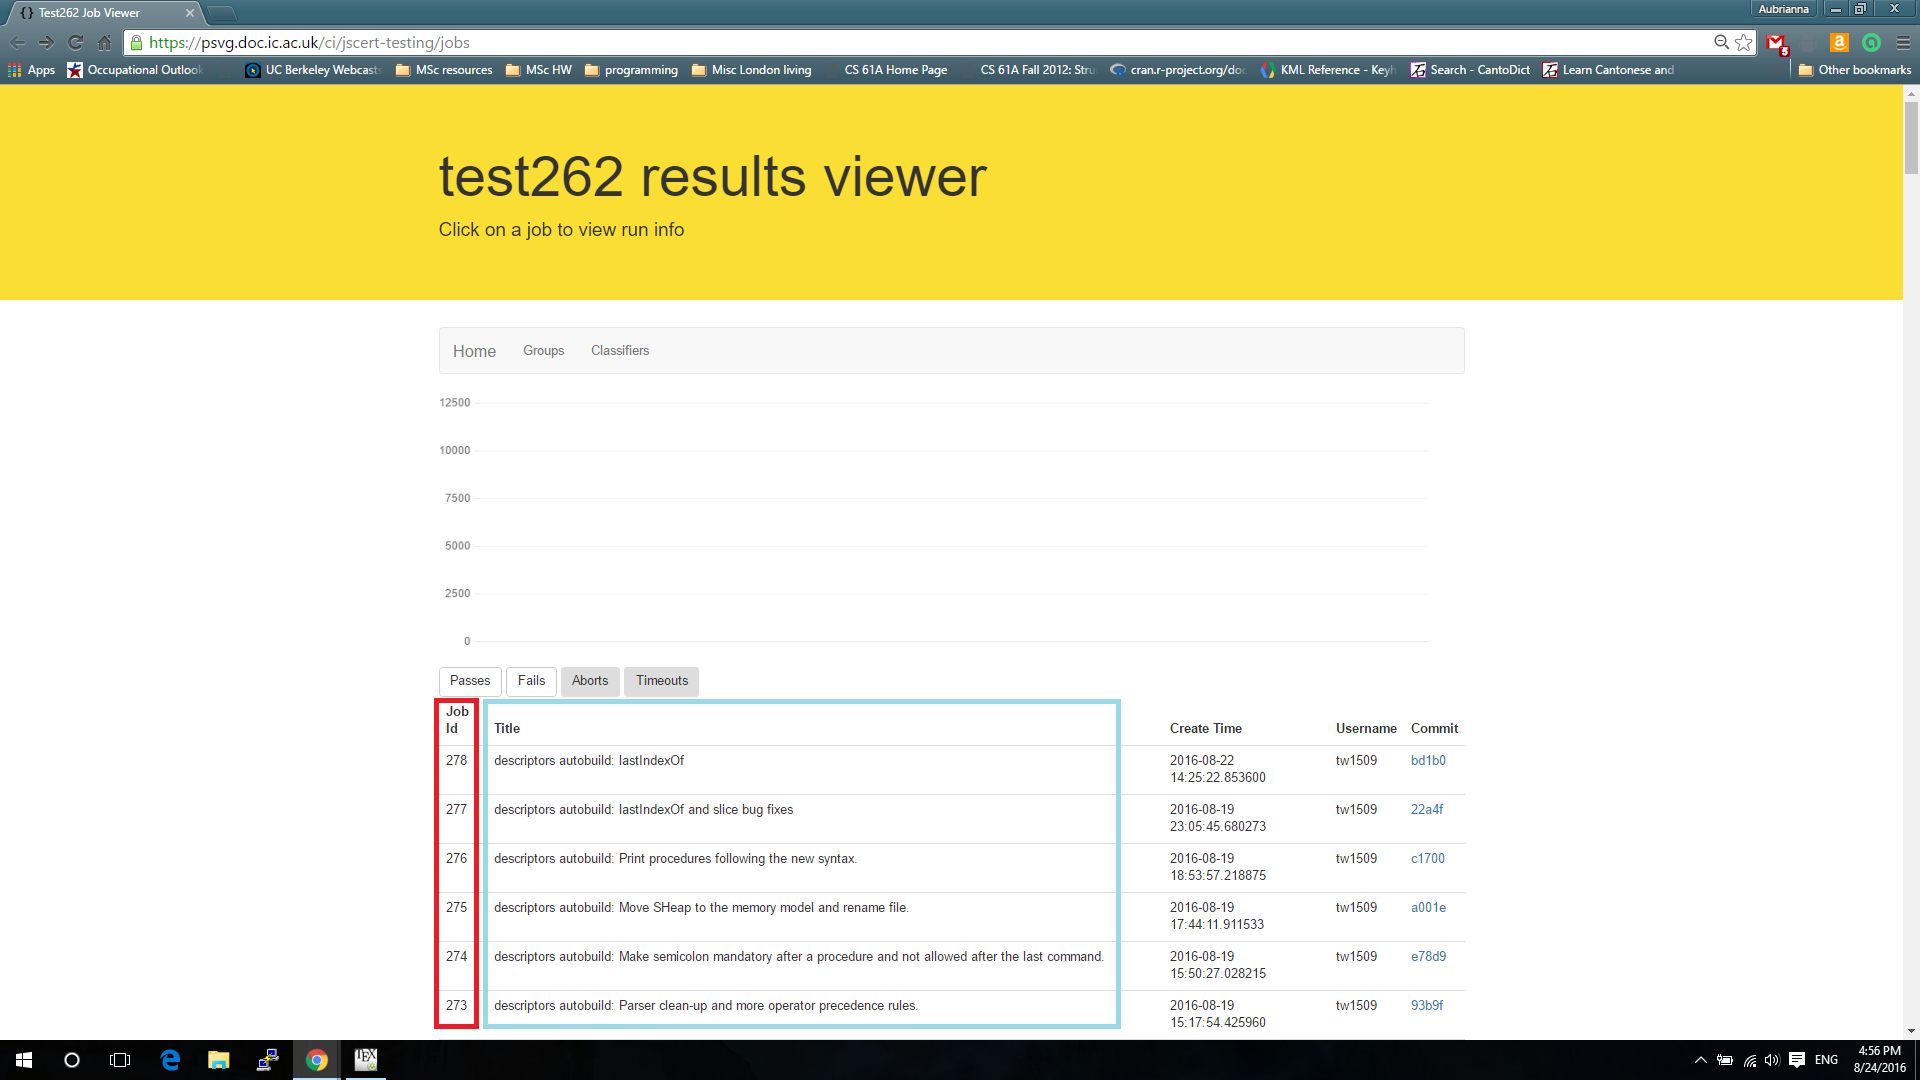
\includegraphics[width=1.0\textwidth]{main_testing_screen_boxed}
\end{figure}

The testing interface can be found at the following web address: https://psvg.doc.ic.ac.uk/ci/jscert-testing/jobs. Figure 11.1 is a screen shot of the landing page of the testing interface. The most important pieces of information on this page are the Job ID, which is boxed in red, and the Title, which is boxed in blue. The Job ID represents the a numbered sequence of Git commits made to the resource-reasoning/JavaScriptVerification project, with the most recent commits at the top of the screen. The Title represents the Git commit message, which ideally includes information about the content of the commit.

\begin{figure}[h!]
  \caption{Individual Job Testing Screen}
  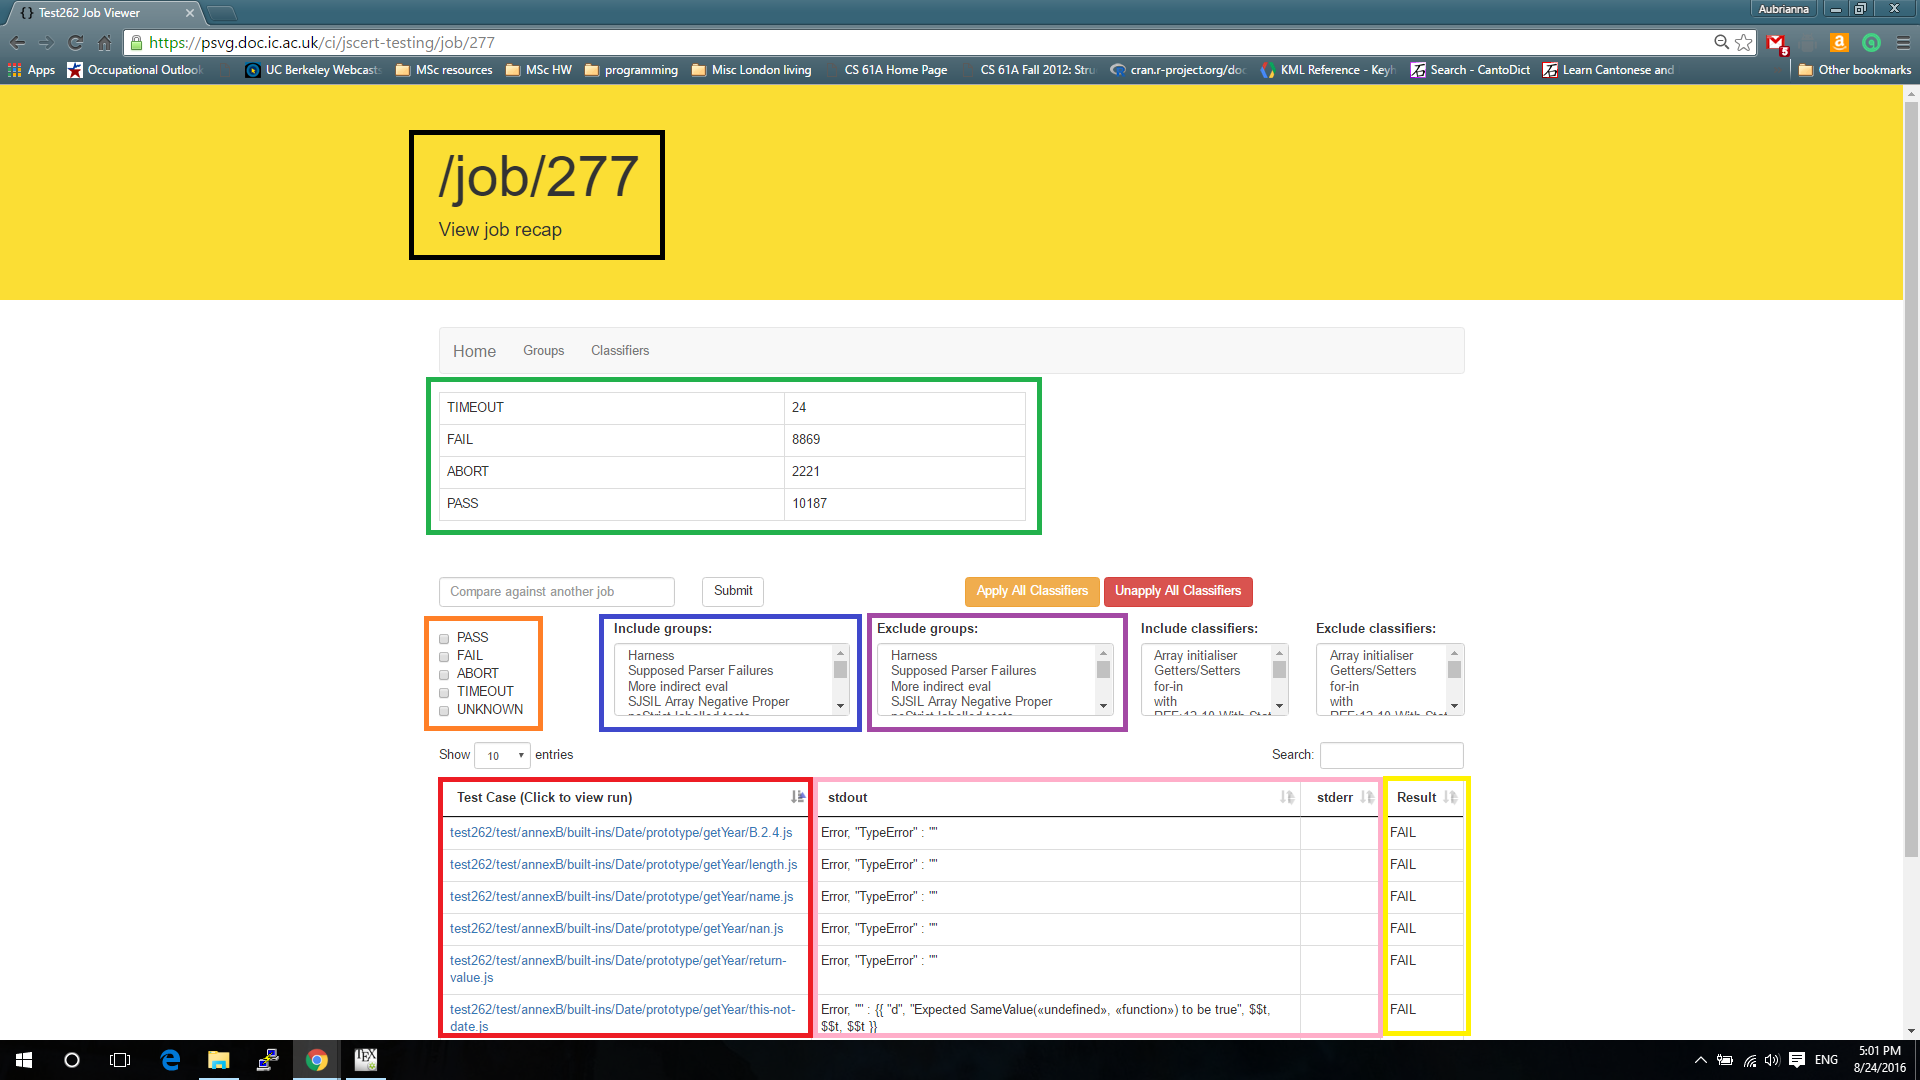
\includegraphics[width=1.0\textwidth]{job_testing_screen_boxed}
\end{figure}

Clicking on either the Job ID or the Title of a commit brings the user to the testing screen for that commit, shown in Figure 11.2. This is the main page for analyzing the tests, and it includes the following pieces of information.

\begin{description}
\item[Job ID] The Job ID is highlighted in black in the header. It shows the user which commit he or she is working with.

\item[Summary Statistics] The summary statistics highlighted in green describes the number of tests in each of the following categories: TIMEOUT, FAIL, ABORT, and PASS. Tests in TIMEOUT are ones that took too long to run, either because the code being tested ran into infinite loops or other such reasons. Tests in FAIL are ones that threw errors into the standard output stream, because the code being tested did not produce the expected results. Tests in ABORT are ones that threw errors into the standard error stream, and they are usually due to JavaScript features that have not yet been implemented in JSIL. Tests in PASSED are ones that produced normal output to the standard output stream with expected results.

\item[Category Checkboxes] The checkboxes highlighted in orange allows the user to filter out tests in one or more specific categories. The first four checkboxes correspond to the categories described previously, and the last checkbox corresponds to the UNKNOWN condition. Tests in UNKNOWN are ones that are still in the queue to be run once a commit is registered on the testing site.

\item[Include Groups] The numerous test cases can be categorized into groups of tests, each targeting a related subset of tests. Most of these groups are created manually, and the creation process will be addressed later. When a group is selected, only the tests belonging to the group will be displayed. Multiple groups can be selected.

\item[Exclude Groups] Groups of tests can be purposefully excluded from the display as well. For example, tests that only pertain to ES6 should be excluded from the analysis because they are outside the scope of this project.

\item[Test Cases] The list of test cases is highlighted in red, and it includes the names of all of the tests the user is looking at. This list includes all of the tests in the test suite by default, and it will be different if the user has included and/or excluded specific groups. Each test is referred to by a test name, which is a hyperlink to a detailed test case page, which will be presented later.

\item[Standard Output and Standard Error] The output of the tests is highlighted in pink, and it includes output to both the standard output stream and the standard error stream. Usually PASSED tests start with "Normal" and the FAILED tests start with "Error" in Stdout, and ABORTED tests start with "Fatal error" in Stderr.

\item[Result] The results are highlighted in yellow, and they show what category the tests fall under.
\end{description} 

\begin{figure}[h!]
  \caption{Test Cases Group}
  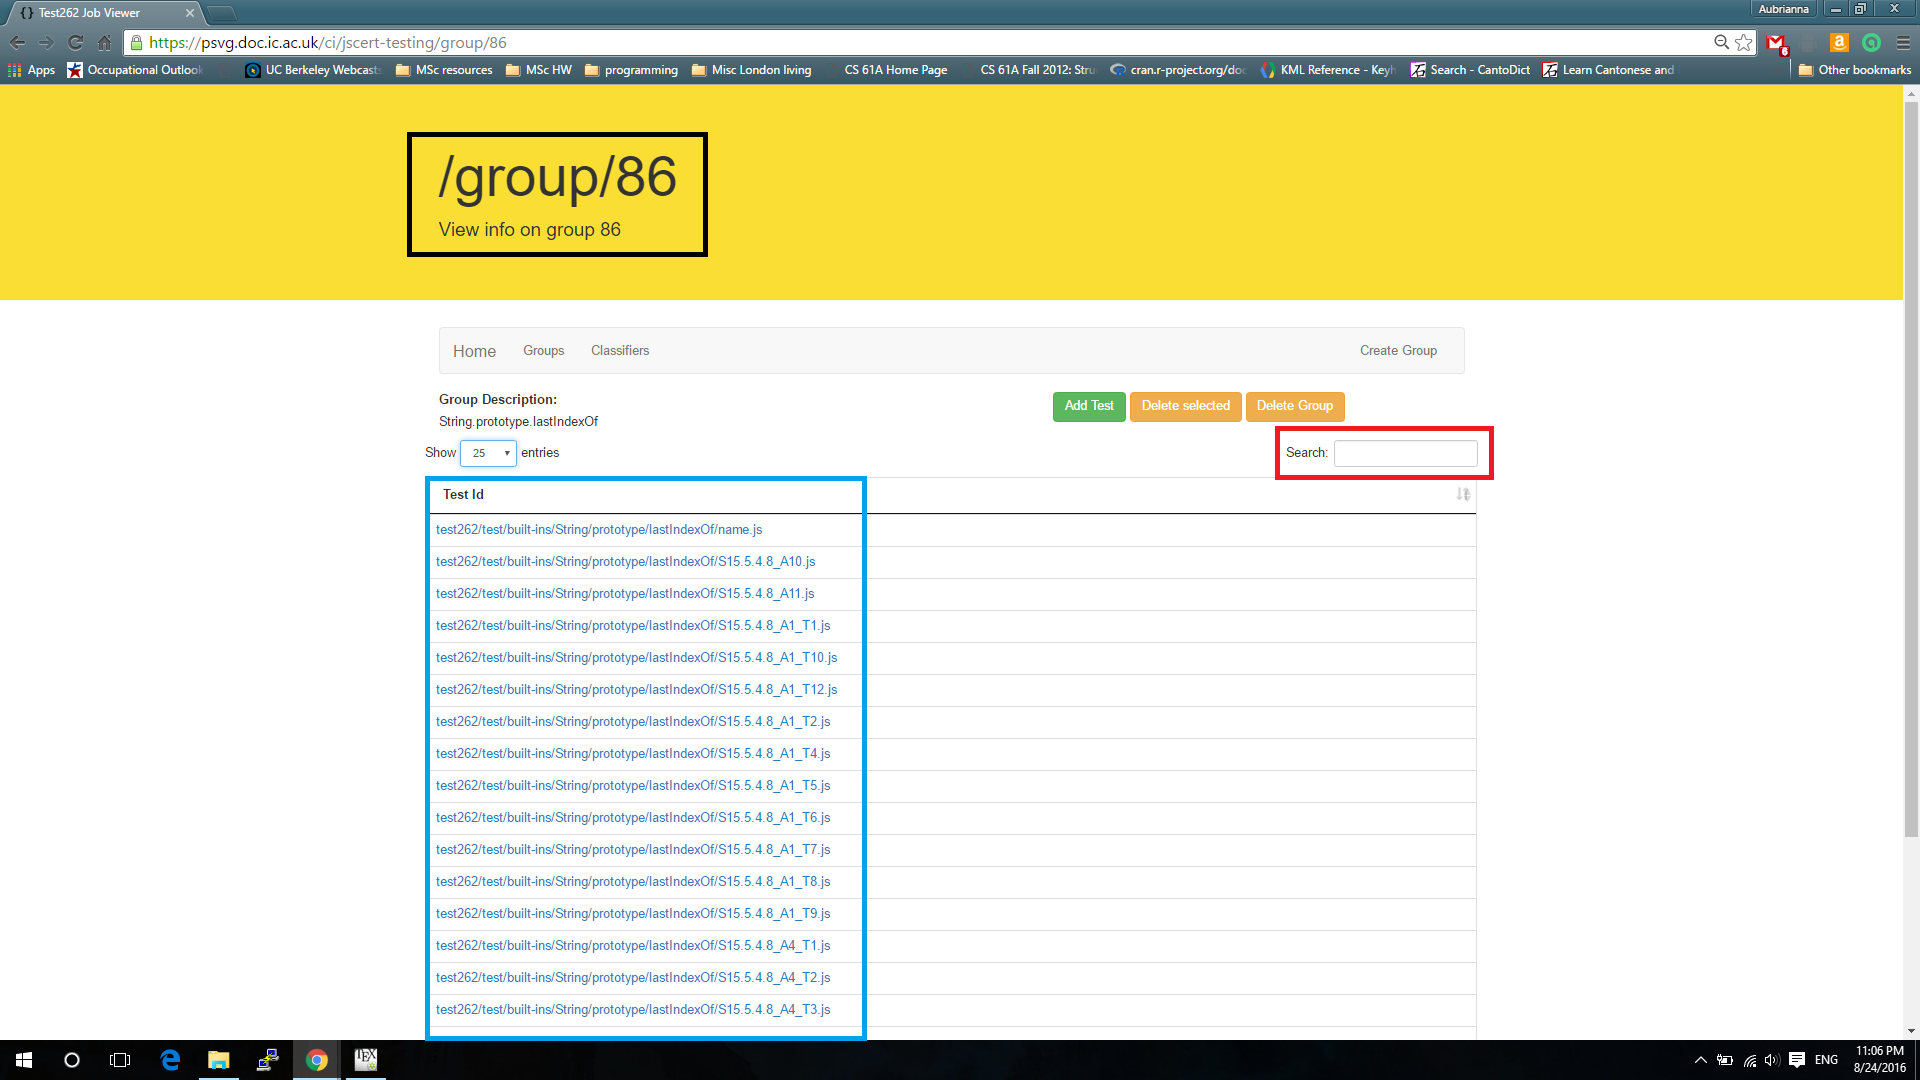
\includegraphics[width=1.0\textwidth]{group_testing_screen_boxed}
\end{figure}

The different test cases groups can be found at https://psvg.doc.ic.ac.uk/ci/jscert-testing/groups/, and from that page, the user can view a specific group like Group 86 presented in Figure 11.3. Highlighted in black in the header is the group number, and highlighted in red is a search box, in which a user can type the name of a test case to see whether a test is already included in the group. The green button for \textbf{Add Test} enables the user to add additional tests into the group. Highlighted in blue is the list of tests belonging to this group. Each test is referred to by a name, and the hyperlink leads the user to a test case history page, which displays the results for this test case for all the recorded test runs. 

\begin{figure}[h!]
  \caption{Test Case Details}
  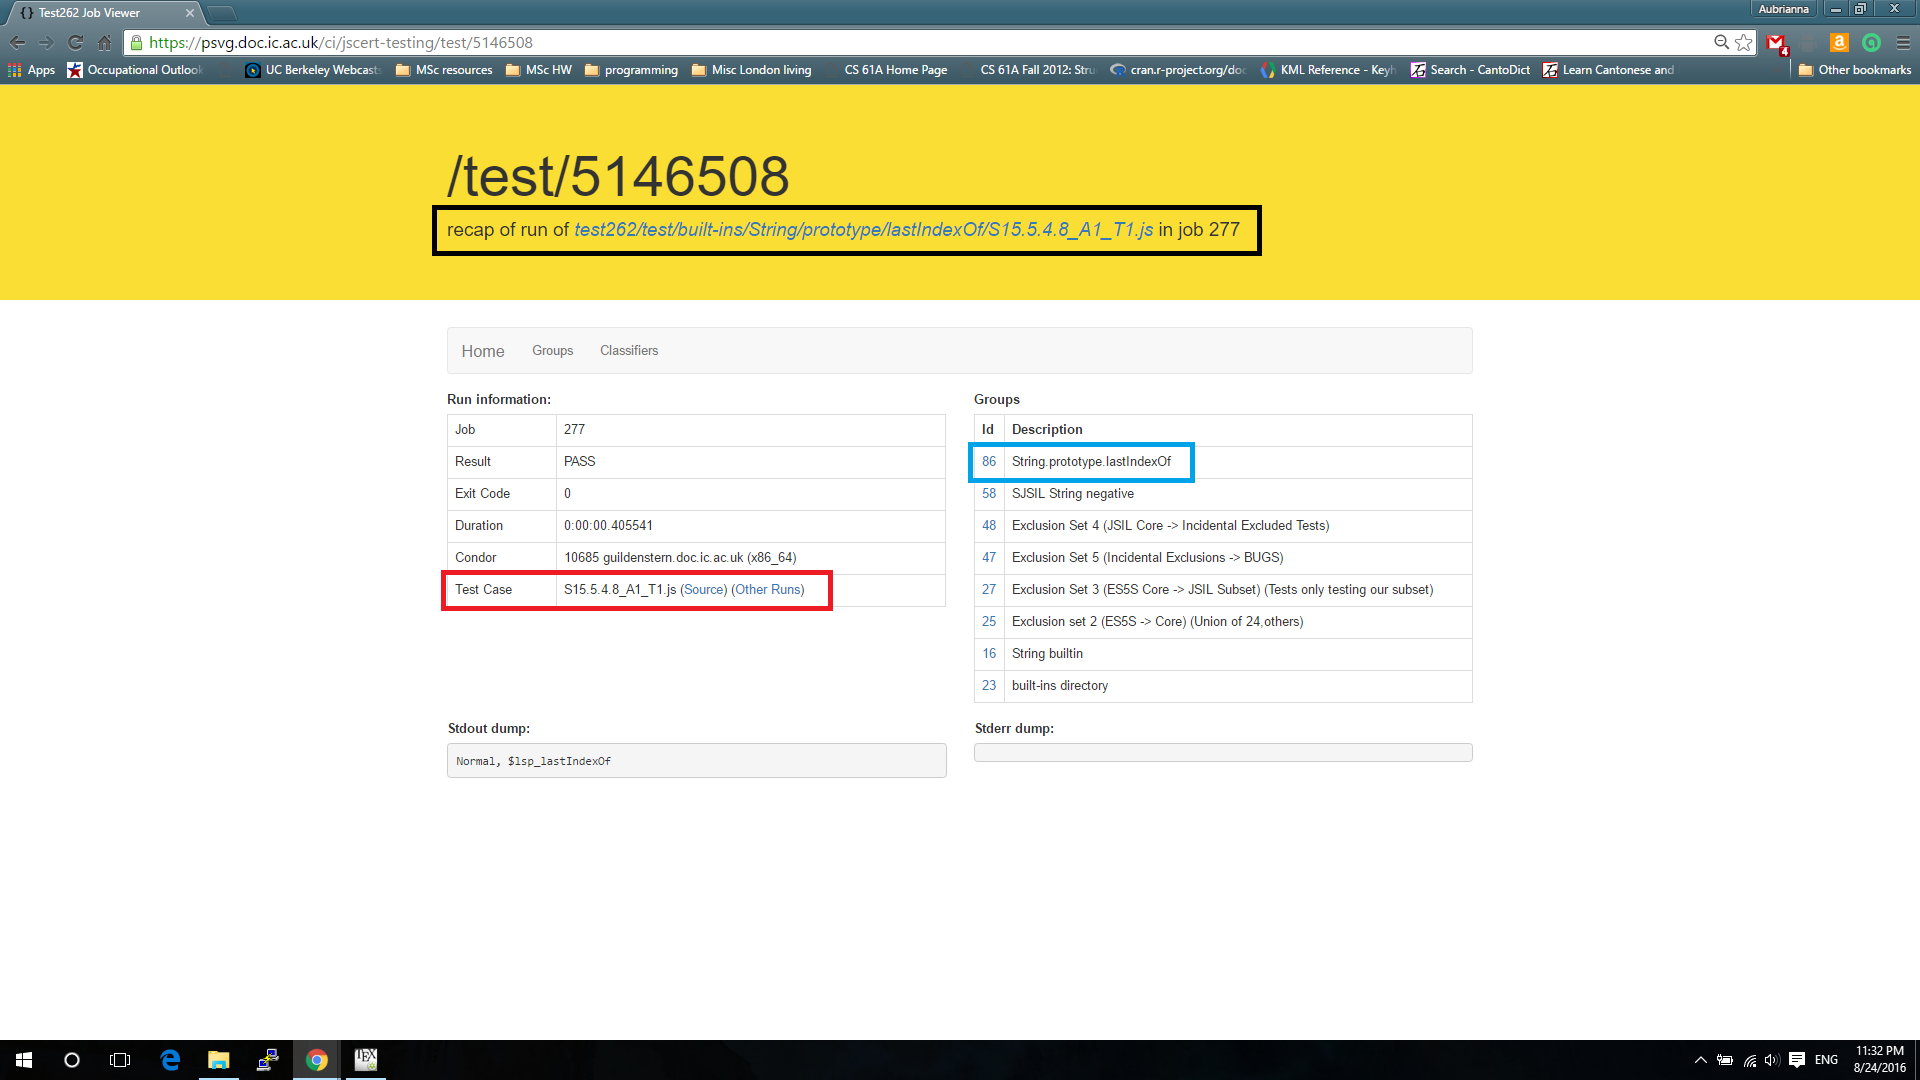
\includegraphics[width=1.0\textwidth]{test_case_testing_screen_boxed}
\end{figure}

If the user clicked the hyperlink on the job page from Figure 11.2, he or she will see a test case details page like the one presented in Figure 11.4. The highlighted black box in the header, as well as the \textbf{Source} text in the red box contain hyperlinks to the source code of the test. The \textbf{Other Runs} text in the red box contains a hyperlink to the test case history page, which is also linked from the test cases group page as mentioned in Figure 11.3. The right hand side shows the group membership of this test, and the group of interest is highlighted in blue.

\begin{figure}[h!]
  \caption{Test Case Source Code}
  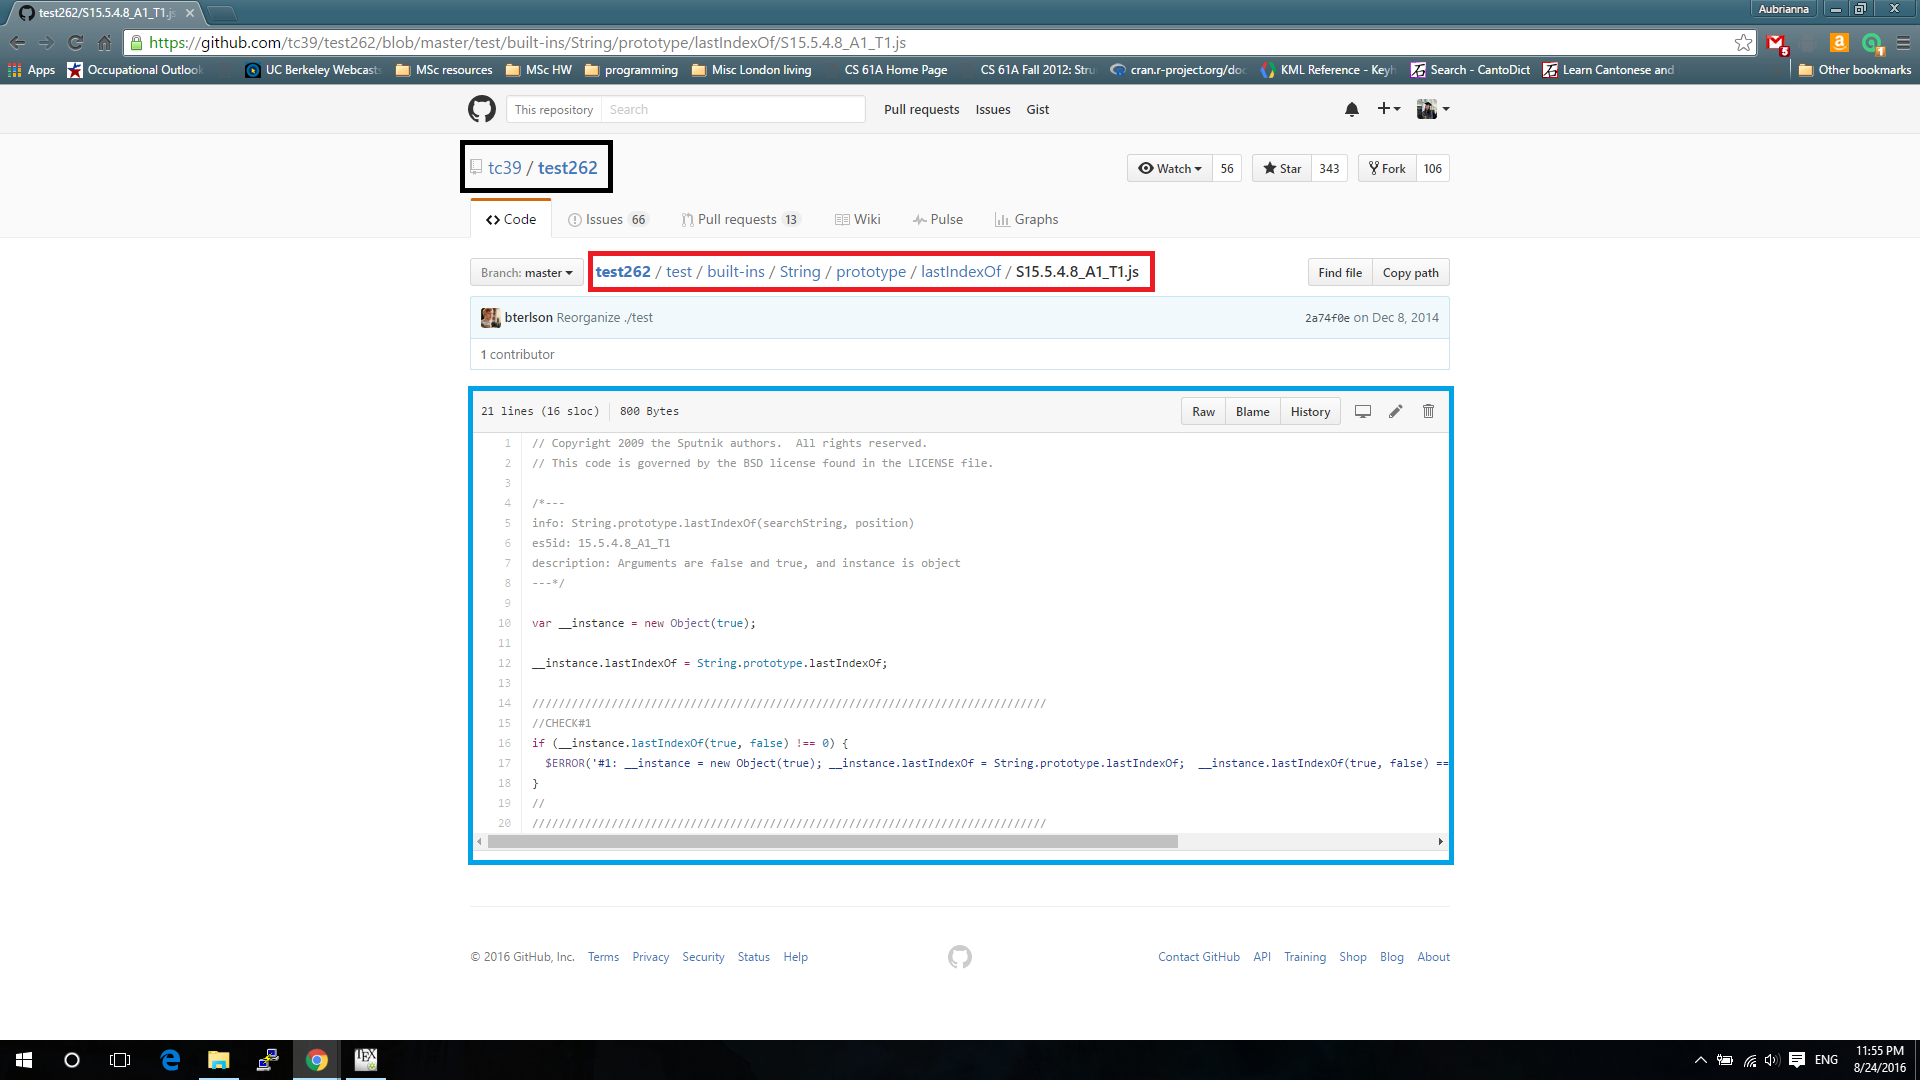
\includegraphics[width=1.0\textwidth]{source_testing_screen_boxed}
\end{figure}

The source code of each test can be viewed on a Github page as shown in Figure 11.5. Highlighted in black on top shows the repository name, which is \textbf{test262}, which belongs to \textbf{tc39}. TC39 refers to Ecma International, Technical Committee 39 - ECMAScript, who are the owner of the \textbf{test262} suite. Highlighted in red is the name of the particular test case, and highlighted in blue is the source code. For tests that produced unexpected behavior, reading the source code to figure out what exactly the test case targets greatly helps in debugging the JSIL program.

%\section{Array Library and Arguments Object}
%\subsection{Array Library}
%%TODO%%???
%\subsection{Arguments Object}

\section{String Library}
As listed in Section~\ref{sec:stringmethods}, six String Library methods were implemented. Tests before implementing any of these methods were analyzed, and five tests have already passed for each method without implementation. Since the tests occur in all methods implemented, the \textbf{METHOD\_NAME} text in the bullet points can be substituted with the actual method names.

\begin{description}
\item[test262/test/built-ins/String/prototype/METHOD\_NAME/S15.5.4.4\_A10.js] This test checks to see if the method's length property is not writable, i.e., its [[writable]] attribute is false. In the implementation, a set of initialization actions have already set this attribute to be false, so this test passed without the actual method implementation.

\item[test262/test/built-ins/String/prototype/METHOD\_NAME/S15.5.4.4\_A11.js] This test checks for the method's length property value. Similarly, this is already determined in the initialization step, and more specifically, the length values for charAt, concat, indexOf, and lastIndexOf are explicitly set to 1, and the length values for slice and substring are set to 2.

\item[test262/test/built-ins/String/prototype/METHOD\_NAME/S15.5.4.4\_A6.js] This test checks to see that the method does not have a prototype property.

\item[test262/test/built-ins/String/prototype/METHOD\_NAME/S15.5.4.4\_A7.js] This test checks to see that the method cannot be used as a constructor to create a new object. When all of these methods are created in the initialization step, their \textbf{construct} property is set to \textbf{empty}, so this test passed without actual method implementation.

\item[test262/test/built-ins/String/prototype/METHOD\_NAME/S15.5.4.4\_A8.js] This test checks to see if the method's length property is not enumerable, i.e., its [[enumerable]] attribute is false. The initialization step also sets this attribute to false, so this test passed before the actual method was implemented.
\end{description}

In addition, for each method there are two tests that have failed before any implementation, because the first is a new ES6 feature, and the second represents a change in program logic from ES5 to ES6.

\begin{description}
\item[test262/test/built-ins/String/prototype/METHOD\_NAME/name.js] In ES6, built-in function objects that are not anonymous functions all have a \textbf{name} property, whose [[value]] attribute is a String value. Its [[writable]] and [[enumerable]] attributes are false by default, and its [[configurable]] attribute is true by default.

\item[test262/test/built-ins/String/prototype/METHOD\_NAME/S15.5.4.4\_A9.js] This test checks to see if the method's length property has the DontDelete attribute. In ES6, String methods' length property do not have the DontDelete attribute, and therefore can be deleted using the \textbf{delete} keyword. In ES5, however, since the length property in each method is not configurable, it cannot be deleted.
\end{description}

\begin{itemize}
\item String.prototype.charAt(pos) \\
In addition to the tests that have already passed and failed, there were 18 tests that were aborted for this method prior to any implementation, for a total of 25 tests. After completing implementation for charAt and rerunning the tests, there were still three ABORTED tests because they utilized the String.prototype.substring method to test charAt, but substring had not been implemented.
\begin{itemize}
\item test262/test/built-ins/String/prototype/charAt/S15.5.4.4\_A4\_T1.js
\item test262/test/built-ins/String/prototype/charAt/S15.5.4.4\_A4\_T2.js
\item test262/test/built-ins/String/prototype/charAt/S15.5.4.4\_A4\_T3.js
\end{itemize}
After completing the substring method, these three tests passed as well. Excluding the nonrelevant tests, all 23 test cases for charAt have passed.
\begin{table}[ht!]
\centering
\begin{subtable}{0.5\textwidth}
\centering
\begin{tabular}{|p{3cm}|p{2cm}|} \hline
\textbf{Test Category} & \textbf{Count} \\ \hline
Pass & 5 \\
Fail & 2 \\
Abort & 18 \\
Timeout & 0 \\
Total & 25 \\ \hline
\end{tabular}
\caption{Before Implementation}
\end{subtable}%
\begin{subtable}{0.5\textwidth}
\centering
\begin{tabular}{|p{3cm}|p{2cm}|} \hline
\textbf{Test Category} & \textbf{Count} \\ \hline
Pass & 23 \\
Fail & 0 \\
Abort & 0 \\
Timeout & 0 \\
Total & 23 \\ \hline
\end{tabular}
\caption{After two rounds of implementations}
\end{subtable}
\caption{String.prototype.charAt(pos)}
\end{table}

\item String.prototype.concat( [ string1 [, string2 [, ...]]] ) \\
The concat method was straightforward. There were 13 ABORTED tests prior to any implementation, and all 13 passed after the first round of coding. Excluding the two nonrelevant tests, all 18 test cases passed for concat.
\begin{table}[ht!]
\centering
\begin{subtable}{0.5\textwidth}
\centering
\begin{tabular}{|p{3cm}|p{2cm}|} \hline
\textbf{Test Category} & \textbf{Count} \\ \hline
Pass & 5 \\
Fail & 2 \\
Abort & 13 \\
Timeout & 0 \\
Total & 20 \\ \hline
\end{tabular}
\caption{Before Implementation}
\end{subtable}%
\begin{subtable}{0.5\textwidth}
\centering
\begin{tabular}{|p{3cm}|p{2cm}|} \hline
\textbf{Test Category} & \textbf{Count} \\ \hline
Pass & 18 \\
Fail & 0 \\
Abort & 0 \\
Timeout & 0 \\
Total & 18 \\ \hline
\end{tabular}
\caption{After Implementation}
\end{subtable}
\caption{String.prototype.concat( [ string1 [, string2 [, ...]]] )}
\end{table}

\item String.prototype.indexOf(searchString, position) \\
In addition to the five PASSED tests and two FAILED tests, indexOf had an additional test in the PASSED category prior to any method implementation.
\begin{itemize}
\item test262/test/built-ins/String/prototype/indexOf/S15.5.4.7\_A1\_T12.js \\
This test checks to see whether an Array Object that included Strings as elements would be indexed correctly. As the Array Library had already been implemented, and it had the ability to hold any type of JavaScript Object in an Array, this test passed without the String method implementation.
\end{itemize}
After the first round of coding, an additional 21 test cases passed, but 7 tests were still in the ABORTED category, because they required additional methods from the Date and String Libraries that are outside the scope of this project. More specifically, one test required the Date.prototype.getTimezoneOffset method, and six tests required the String.fromCharCode method. Excluding the two nonrelevant tests, there were a total of 27 PASSED tests and 7 ABORTED tests for a total of 34 test cases.
\begin{table}[ht!]
\centering
\begin{subtable}{0.5\textwidth}
\centering
\begin{tabular}{|p{3cm}|p{2cm}|} \hline
\textbf{Test Category} & \textbf{Count} \\ \hline
Pass & 6 \\
Fail & 2 \\
Abort & 28 \\
Timeout & 0 \\
Total & 36 \\ \hline
\end{tabular}
\caption{Before Implementation}
\end{subtable}%
\begin{subtable}{0.5\textwidth}
\centering
\begin{tabular}{|p{3cm}|p{2cm}|} \hline
\textbf{Test Category} & \textbf{Count} \\ \hline
Pass & 27 \\
Fail & 0 \\
Abort & 7 \\
Timeout & 0 \\
Total & 34 \\ \hline
\end{tabular}
\caption{After Implementation}
\end{subtable}
\caption{String.prototype.indexOf(searchString, position)}
\end{table}

\item String.prototype.lastIndexOf(searchString, position) \\
Similar to indexOf, lastIndexOf also had six passing tests before any method implementation, and the test case below also tested for whether an element in an Array Object can be correctly identified from the lastIndexOf operation.
\begin{itemize}
\item test262/test/built-ins/String/prototype/lastIndexOf/S15.5.4.8\_A1\_T12.js
\end{itemize}
After the first round of coding, 10 additional tests passed, and the 4 tests below failed. 
\begin{itemize}
\item test262/test/built-ins/String/prototype/lastIndexOf/S15.5.4.8\_A1\_T1.js \\
This test creates an Object with the boolean value \textbf{true}, and tries to find the index of \textbf{true} within the Object instance, provided the Object's lastIndexOf method is the same as String's lastIndexOf method. Upon analyzing the test source code and the JSIL implementation, it was discovered that the JSIL logic was incorrectly implemented. The first version of the JSIL lastIndexOf could not handle cases where the searchString was the same length or larger than the String Object performing the method.
\item test262/test/built-ins/String/prototype/lastIndexOf/S15.5.4.8\_A1\_T2.js \\
This test creates a Boolean Object, and sets the Object's lastIndexOf method to be that of String's. Because the default value for a Boolean Object is \textbf{false}, when the lastIndexOf method is called on the Boolean Object, passing in inputs that essentially reduce to \textbf{false} should find a match at the beginning of the string. This case is similar to the previous one, and was fixed by handling searchString inputs of the same size as the String Object itself.
\item test262/test/built-ins/String/prototype/lastIndexOf/S15.5.4.8\_A1\_T10.js \\
This test checks to see if looking for a searchString from a position that is not a number, i.e., \textbf{NaN}, would produce the correct results. The initial JSIL implementation incorrectly disregarded the step to check whether the position parameter is not a number, whereas the correct implementation should convert \textbf{NaN} to positive infinity.
\item test262/test/built-ins/String/prototype/lastIndexOf/S15.5.4.8\_A4\_T3.js \\
This test creates a searchString and an empty Object as the index position. Upon inputting these parameters into a String value calling its lastIndexOf method, the empty Object should be converted to \textbf{NaN}, and the rest of the logic is as presented for the previous test case.
\end{itemize}
Two rounds of bug-fixing and re-testing resulted in their passing. In the end, excluding nonrelevant test cases, all 20 test cases passed.
\begin{table}[ht!]
\centering
\begin{subtable}{0.5\textwidth}
\centering
\begin{tabular}{|p{3cm}|p{2cm}|} \hline
\textbf{Test Category} & \textbf{Count} \\ \hline
Pass & 6 \\
Fail & 2 \\
Abort & 14 \\
Timeout & 0 \\
Total & 22 \\ \hline
\end{tabular}
\caption{Before Implementation}
\end{subtable}%
\begin{subtable}{0.5\textwidth}
\centering
\begin{tabular}{|p{3cm}|p{2cm}|} \hline
\textbf{Test Category} & \textbf{Count} \\ \hline
Pass & 20 \\
Fail & 0 \\
Abort & 0 \\
Timeout & 0 \\
Total & 20 \\ \hline
\end{tabular}
\caption{After two rounds of implementations}
\end{subtable}
\caption{String.prototype.lastIndexOf(searchString, position)}
\end{table}

\item String.prototype.slice(start, end) \\
Before any method implementation, there were five PASSED tests, two FAILED tests, and 27 ABORTED tests. After the first round of coding, 14 additional tests passed, but 13 were still aborted. 
\begin{itemize}
\item test262/test/built-ins/String/prototype/slice/S15.5.4.13\_A1\_T5.js \\
This test sets the Function prototype slice method to the String prototype slice method, but since the function object constructor had not been implemented, it was impossible to run this test.
\item test262/test/built-ins/String/prototype/slice/S15.5.4.13\_A1\_T14.js \\
This test passes an empty function object into the slice method of a String value, and this empty Object should be converted into \textbf{NaN}. The initial JSIL implementation only took into account cases where the start parameter can be successfully converted to an integer value, thus it failed when trying to index on \textbf{NaN}. Changes to the code was made to set the start value to be the beginning of the String if the start input cannot be successfully converted to an integer.
\item test262/test/built-ins/String/prototype/slice/S15.5.4.13\_A1\_T15.js \\
This test creates a Number Object, sets its prototype.slice method to be that of String's prototype.slice, and calls the method with no inputs. Similar to the previous test case, the initial JSIL implementation failed because an empty argument cannot be transformed into an integer.
\item test262/test/built-ins/String/prototype/slice/S15.5.4.13\_A1\_T6.js \\
This test attempts to pass \textbf{Undefined} into the slice method as the start input, and was similarly fixed by setting a default start value.
\item test262/test/built-ins/String/prototype/slice/S15.5.4.13\_A2\_T1.js \\
This test creates a String Object, slices the entire String, and checks to see if the \textbf{typeof} value for this Object is the value "string". The test calls the slice method with no inputs, so the start value should be taken as the beginning of the String by default, and this test was similarly fixed by setting a default start.
\end{itemize}

The following test cases were aborted because of a mistake of variable name referencing in the JSIL implementation. JSIL has an internal indexing mechanism for strings, which only takes positive integers as input for indices, but the initial JSIL implementation incorrectly used the direct input value, rather than the calculated value, as the string index. In addition, when the start and end inputs vary by more than one index value, the start index is incremented to get the consecutive string characters until the end index is reached. In the first JSIL implementation, however, an incorrect start index was incremented.
\begin{itemize}
\item test262/test/built-ins/String/prototype/slice/S15.5.4.13\_A1\_T1.js \\
This test inputs the boolean values false and true into the slice method. When indexing the string in JSIL, the initial JSIL function used the boolean value, rather than an integer converted from this boolean. Hence JSIL was unable to provide the string character at the given start index.
\item test262/test/built-ins/String/prototype/slice/S15.5.4.13\_A1\_T2.js \\
This test uses a function object that returns the boolean value true as the start value given to the slice method, and thus JSIL was unable to correctly index the string.
\item test262/test/built-ins/String/prototype/slice/S15.5.4.13\_A1\_T8.js \\
This test used a negative integer as the start input, and JSIL requires nonnegative indices for strings.
\item test262/test/built-ins/String/prototype/slice/S15.5.4.13\_A2\_T2.js \\
This test uses \textbf{NaN} as the start input, which is not an integer and therefore could not be used as a string index in JSIL.
\item test262/test/built-ins/String/prototype/slice/S15.5.4.13\_A3\_T3.js \\
This test uses negative infinity as the start input, which is not an integer and therefore could not be used as a string index in JSIL.
\item test262/test/built-ins/String/prototype/slice/S15.5.4.13\_A1\_T4.js \\
This test uses \textbf{null} as the start input, which is not an integer and therefore could not be used as a string index in JSIL.
\item test262/test/built-ins/String/prototype/slice/S15.5.4.13\_A1\_T7.js \\
This test uses a string value as the start input, therefore it could not be used as a string index in JSIL.
\item test262/test/built-ins/String/prototype/slice/S15.5.4.13\_A1\_T10.js \\
This test uses a function object as the start input, therefore it could not be used as a string index in JSIL.
\end{itemize}

After fixing the above-mentioned issues, only one test remained in the ABORTED state, but since its passing requires the function object constructor, it is out of the scope of this project and is therefore left unimplemented. Otherwise, there remain 31 relevant test cases, all of which were in PASSED.
\begin{table}[ht!]
\centering
\begin{subtable}{0.5\textwidth}
\centering
\begin{tabular}{|p{3cm}|p{2cm}|} \hline
\textbf{Test Category} & \textbf{Count} \\ \hline
Pass & 5 \\
Fail & 2 \\
Abort & 27 \\
Timeout & 0 \\
Total & 34 \\ \hline
\end{tabular}
\caption{Before Implementation}
\end{subtable}%
\begin{subtable}{0.5\textwidth}
\centering
\begin{tabular}{|p{3cm}|p{2cm}|} \hline
\textbf{Test Category} & \textbf{Count} \\ \hline
Pass & 31 \\
Fail & 0 \\
Abort & 1 \\
Timeout & 0 \\
Total & 32 \\ \hline
\end{tabular}
\caption{After two rounds of implementations}
\end{subtable}
\caption{String.prototype.slice(start, end)}
\end{table}

\item String.prototype.substring(start, end) \\
The substring method was relatively straightforward as well. There were 35 ABORTED tests before method implementation, and after the first round of coding, one test remained ABORTED. 
\begin{itemize}
\item test262/test/built-ins/String/prototype/substring/S15.5.4.15\_A1\_T5.js \\
This test sets the Function prototype substring method to the String prototype substring method, but since the function object constructor had not been implemented, it was impossible to run this test.
\end{itemize}
Excluding the nonrelevant tests, there were a total of 40 test cases, of which 39 passed, and one aborted.
\begin{table}[ht!]
\centering
\begin{subtable}{0.5\textwidth}
\centering
\begin{tabular}{|p{3cm}|p{2cm}|} \hline
\textbf{Test Category} & \textbf{Count} \\ \hline
Pass & 5 \\
Fail & 2 \\
Abort & 35 \\
Timeout & 0 \\
Total & 42 \\ \hline
\end{tabular}
\caption{Before Implementation}
\end{subtable}%
\begin{subtable}{0.5\textwidth}
\centering
\begin{tabular}{|p{3cm}|p{2cm}|} \hline
\textbf{Test Category} & \textbf{Count} \\ \hline
Pass & 39 \\
Fail & 0 \\
Abort & 1 \\
Timeout & 0 \\
Total & 40 \\ \hline
\end{tabular}
\caption{After Implementation}
\end{subtable}
\caption{String.prototype.substring(start, end)}
\end{table}

\end{itemize}

%%%%%%%%%%%%%%%%%%%%%%%%%%%%%%%%%%%%
\chapter{Conclusion}
\section{Project Summary and Contributions}
This report has described the importance of JavaScript in modern day web computing and provided a sample of previous verification projects for not only JavaScript, but also a variety of other programming languages. This project stemmed from previous work done on JSCert and JSRef, a mechanized specification of the ECMAScript standard and its reference interpreter. Separation logic has been used to reason about JavaScript programs, modeling program execution based on a heap structure. This project has also relied on the use of operational semantics to clarify and mechanize the ECMAScript specification written in English. Indeed, JSCert itself uses pretty big step operational semantics to cover the language constructs in JavaScript. 

The report went on to describe various JavaScript constructs, such as strict mode, Objects and properties, prototype inheritance, and the JavaScript heap, before moving on to describe JSIL as a language. The benefits of utilizing JSIL as an intermediate language include its simplified control flow based on a goto syntax, the elimination of nested procedures, while still preserving extensible objects and dynamic properties, make logical analysis of JSIL programs easier yet still correct with respect to the corresponding JavaScript programs.

The main contributions of this project are the implementations for the Object.prototype, Array, part of the String libraries, and the arguments object in JSIL. A total of 35 library methods were implemented, enabling the passage of more than 2,200 test cases in the ECMAScript Test262 test suite. The details of each library method --- its syntax, purpose, expected result, and sample usage --- were listed in each library's corresponding chapter, and the testing process was described in detail for the String library methods. For selected methods in the Object.prototype and Array libraries, the ECMAScript standard specification, pretty big step operational semantics, as well as JSIL implementation were described in detail.

The completion of this project marked the end of implementing the core language constructs as well as the most critical built-in libraries of JavaScript in JSIL. The only portions of the JSIL reference implementation that remain to be completed are the Function constructor and parts of the String library.

\section{Evaluation}
The process of implementation was streamlined in the order of reading the ECMAScript standard --- creating JavaScript unit tests --- coding in JSIL --- running JavaScript unit tests based on the JSIL implementation --- running Test262 on the JSIL implementation. Each component of this process is evaluated in the following paragraphs.

Understanding the ECMAScript standard for the libraries and constructs has mostly been straightforward, although certain methods, such as Array.prototype.sort and String.prototype.indexOf, did not provide specific implementation details, but rather only outlined the desired actions to be accomplished. As such, there was freedom to implement as the author saw fit, in terms of efficiency or code clarity. For example, the quicksort algorithm was chosen for Array.prototype.sort, even though other sorting algorithms, such as insertion sort and merge sort were also available alternatives.

The original intent of learning operational semantics was to create a mechanized version of the ECMAScript specification, in order to clarify procedures for when the specification is ambiguous. During this project, however, the ECMAScript standard has mostly been clear enough that creating operational semantics was not necessary. It would have been helpful to create operational semantics for the methods without specific implementation details described previously, but pseudocode was used as an alternative to clarify procedure actions. Also, as creating operational semantics was a difficult task in itself, it provided little benefit to the implementation process as a whole. Operational semantics was, however, produced for the methods that were presented in detail for this report as a learning exercise, and it was used to show the close correspondence between the JSIL implementation and the ECMAScript standard.

Creating and running JavaScript unit tests have also been fairly straightforward, as basic JavaScript programs are easy to write, demanding only ingenuity to cover corner cases. The results of using unit tests before the Test262 suite have been positive, as the unit tests often uncovered most bugs in the JSIL implementation before committing changes to the repository. As a result, many library methods passed all the corresponding tests in the official test suite the first time through, and the other methods required few bug fixes since fixing one component in JSIL often fixed all failing test cases. Indeed, putting in the effort to systematically sanity check the JSIL implementation using unit tests significantly decreased the risk of drastic or complicated bug fixes.

The main difficulties regarding coding in JSIL were threefold --- first was the initial learning curve to master a goto language, and second was understanding the error messages from the parser, and third was keeping up with changes in the language made by other members of the research group. Coding in a goto language was practiced alongside reading operational semantics rules for the internal methods of JavaScript. During coding, however, unexpected error messages could appear, that sometimes did not correspond to the actual error, or gave no additional information than simply, ``syntax error". Thus, debugging could be difficult because there was little external sources, such as Stack Overflow, for help due to the nature of JSIL as a research language. Lastly, as the language is constantly evolving, keeping abreast of the changes in order to always write correct code was challenging since changes made by other members of the research group sometimes went unnoticed, until an error message came up. 

In terms of forecasting the workload, most estimations have been reasonable, and deadlines set in the first report have been met satisfactorily. Implementation of the arguments object, however, took significantly less time than expected. Originally, the arguments object was thought to be rather complicated, as it is an important construct and thus assumed to have required changes to the underlying JSIL model. After understanding the ECMAScript specification, however, the strict mode version of the arguments object turned out to be much simpler than expected, requiring only about 30 lines of JSIL code to implement. Thus, a couple weeks' worth of time was freed up to take on a subset of the String library, which was not initially included in the project proposal, enabling additional passing tests for the Test262 suite.

\section{Future Work}
Continuing with the direction of this project, there is additional work to be done to implement the rest of the JavaScript libraries in JSIL, including but not limited to the Number, rest of String, Date, and RegExp libraries. But although these libraries are worth implementing, they are not crucial to the progress of the verification tool based on the JSIL language.

\begin{description}
\item[Number] The Number library includes four methods spanning four pages in the ECMAScript specification that remain to be completed. 
\item[String] The String library includes nine methods unrelated to the RegExp library and two methods related to it spanning seven pages of the specification that remain to be completed.
\item[Date] The Date library has not been worked on, and it includes 15 Date-related constructs and 52 methods within 16 pages in the specification.
\item[RegExp] The RegExp library has not been worked on, and it includes 19 RegExp-related constructs and six methods for a total of 18 pages in the specification.
\end{description}

On the other hand, future work regarding the verification goal include completing a prototype of a semiautomatic verification tool, called JaVerT. This tool makes use of JSIL's reference implementation of JavaScript language constructs and libraries, and aims to verify the axiomatic specification of JSIL's internal and library implementations. The end goal of the verification project is to eventually be able to verify large JavaScript programs automatically, and colossal efforts toward that direction have been made continually by other members of the research group.

%%%%%%%%%%%%%%%%%%%%%%%%%%%%%%%%%%%%%
%% bibliography
\bibliographystyle{plain}
\bibliography{refs}

\end{document}
